\chapter{Elements of quantum information with continuous variables}
    This chapter gives a brief overview of quantum mechanics postulates,
    of the notation and of the essential concept used in this thesis. 
    The target of that is to explain to the reader the essential concept of quantum mechanics
    and of quantum continuous-variable states, in 
    order to give him the possibility to understand the obtained result.

    \section{Preliminaries on quantum mechanics}
    For understand the important results about the communication with continuos
    states, it is essential to give a brief introduction about the main aspects 
    of quantum mechanics theory.
    This theory is based on a solid mathematic framework presented in this section.
    It is impossible to discuss about quantum mechanics without its mathematical 
    formalism.
    
    \subsection{Postulates}
    Like every phisics theory, quantum mechanics is builded from few 
    essential postulates.
    In this section are briefly introduced the six Dirac-Von Newman 
    postulates of Quantum Mechanics \cite{quantumMec_Dirac,quantumMec_Neumann}.

    \begin{postulate}[State Representation]
        The state of an isolated quantum system is represented by a complex unitary 
        vector $\ket{\psi}$ in an Hilbert space $\Hilbert$.
        The space of possible states of the system is called state space and it is a
        separable complex Hilbert space.
        \label{post:1}
    \end{postulate}
    Every ket-vector $\ket{\psi} \in \Hilbert$ can be represented as a column vector 
    $\ket{\psi}=\left[ a_1,a_2,\dots,a_N \right]$, where $N$ is the dimension of the 
    state space $\Hilbert$. The bra-vector $\bra{\psi}$ is the correspondent vector of
    $\ket{\psi}$ in the dual-space of $\Hilbert$ and can be represented as the 
    transposed conjugate of $\ket{\psi}$.

    Differently from the classical physics, in quantum mechanics the concept
    of state of system is introduced. In classical mechanics a system is 
    described by his observables, like position or four-wheeled.
    
    \begin{postulate}[Observables]
        Every observables of the system is represented by an Hermitian operator 
        $\Operator{M}:\Hilbert\to\Hilbert$ acting on the state space.
        The outcomes of the measurement can only be one of the eigenvalue of the 
        operator $\Operator{M}$.
        \label{post:2}
    \end{postulate}
    The possible outcomes of the measurement are real number because $\Operator{M}$
    is self-andjoint. 

    \begin{postulate}[Born's Rule]
        The probability to get the measurement $\lambda_i$ from the observable 
        $\Operator{M}$ in the system in state $\ket{\psi}$ is:
        \begin{equation*}
            %\mathbb{P}(\lambda_i)=\braket{\psi}{\lambda_i}\braket{\lambda_i}{\psi}
            \mathbb{P}(\lambda_i)=\bra{\psi}\Operator{P}_i\ket{\psi}
        \end{equation*}
        where $\bra{\psi}$ is the correspondent vector of $\ket{\psi}$ in the 
        dual space of $\Hilbert$ and where $\Operator{P}_i$ is the projection operator
        of $\lambda_i$ in the correspondent space.
        \label{post:3}
    \end{postulate}

    \begin{postulate}[Wavefunction Collapse]
        The state $\ket{\psi'}$ after measurement of $\lambda_i$ is $\Operator{P}_i\ket{\psi}$ (with the
        necessary normalization):
        \begin{equation*}
            \ket{\psi'}=\frac{\Operator{P}_i\ket{\psi}}{\bra{\psi}\Operator{P}_i\ket{\psi}}.
        \end{equation*}
        \label{post:4}
    \end{postulate}

    \begin{postulate}[Time Evolution]
        The time evolution $\ket{\psi(t)}$ of an isolated quantum system is given by an unitary operator
        $\Operator{U}$:
        \begin{equation*}
            \ket{\psi(t)}=\Operator{U}(t_0,t)\ket{\psi(t_0)}.
        \end{equation*}
        \label{post:5}
    \end{postulate}
    From postulate \ref{post:5}, it is possible to obtain the \emph{time dependent Shrodinger Equation}:
    \begin{equation}
        i\hbar\partialderivative{}{t}\ket{\psi(t)}=\Operator{H}(t)\ket{\psi(t)}
    \end{equation}
    where $\Operator{H}(t)$ is the Hamiltonian matrix, $\hbar$ is the reduced Planck's constant and $i=\sqrt{-1}$
    is the immaginary unit.

    \begin{postulate}[Composite System]
        The state space $\Hilbert$ of a system composed of $\Hilbert_1$ and $\Hilbert_2$ is given by
        \begin{equation*}
            \Hilbert=\Hilbert_1\otimes\Hilbert_2.
        \end{equation*}
        \label{post:6}
    \end{postulate}

    \subsection{The density operator}
    \label{TheDensOp}
    The last postulate \ref{post:6} has very important consequences for composite system. It is possible
    to describe two tipes of combined systems:

    \begin{definition}[Product states]
        A state $\ket{\psi}\in\Hilbert$ with $\Hilbert=\Hilbert_1\otimes\Hilbert_2$ is a
        pure state if exists $\ket{\psi_1}\in\Hilbert_1$ and $\ket{\psi_2}\in\Hilbert_2$
        such that:
        \begin{equation*}
            \ket{\psi}=\ket{\psi_1}\otimes\ket{\psi_2}.
        \end{equation*}
        \label{def:1}
    \end{definition}
    A product state represents two systems which do not interact; an operation on one of 
    them does not perturb the other.

    \begin{definition}[Entengled states]
        A system that is not in a product state (\ref{def:1}), is in an entengled state. 
        \label{def:2}
    \end{definition}
    When a system is in an entengled state it is not possible to characterize the two subsystems
    with the states vector, although the state vector of the composite system is known.

    \paragraph{Density operator}\mbox{}\\
        For a more general treatment, the following representation of states is given:
        \begin{definition}
            The state of quantum system is described by a linear operator $\Operator{\varXi}:\Hilbert\to\Hilbert$, 
            called density operator such that 
            $\Operator{\varXi}^\dagger=\Operator{\varXi}$ and $\tr{\Operator{\varXi}}=1$.
            \label{def:3}
        \end{definition}
        According to the definition \ref{def:3}, the postulates \ref{post:3}, \ref{post:4},
        \ref{post:5} can be reformulate as following.\par
        The probability to get the measurement $\lambda_i$ from the observable 
        $\Operator{M}$ in the system in state $\Operator{\varXi}$ is:
        \begin{equation}
            \mathbb{P}(\lambda_i)=\tr{\Operator{\varXi}\Operator{P}_i}.
            \label{post:3.1}
        \end{equation}
        The state $\Operator{\varXi'}$ after measurement of $\lambda_i$ is give by:
        \begin{equation}
            \Operator{\varXi'}=\frac{\Operator{P}_i\Operator{\varXi}\Operator{P}_i^\dagger}
            {\tr{\Operator{P}_i\Operator{\varXi}\Operator{P}_i^\dagger}}.
            \label{post:4.1}
        \end{equation}
        The time evolution $\Operator{\varXi}(t)$ of an isolated quantum system is given by an unitary operator
        $\Operator{U}$ as:
        \begin{equation}
            \Operator{\varXi}(t)=\Operator{U}\Operator{\varXi}(t_0)\Operator{U}^\dagger.
            \label{post:5.1}
        \end{equation}

    %\section{Combining Systems}
The last postulate \ref{post:6} has very important consequences for composite system. It is possible
to describe two tipes of combined systems:

    \begin{definition}[Product states]
        A state $\ket{\psi}\in\Hilbert$ with $\Hilbert=\Hilbert_1\otimes\Hilbert_2$ is a
        pure state if exists $\ket{\psi_1}\in\Hilbert_1$ and $\ket{\psi_2}\in\Hilbert_2$
        such that:
        \begin{equation*}
            \ket{\psi}=\ket{\psi_1}\otimes\ket{\psi_2}.
        \end{equation*}
        \label{def:1}
    \end{definition}
    A product state represents two states which do not interact; an operation on one of 
    them does not perturb the other.

    \begin{definition}[Entengled states]
        A system that is not in a product state (\ref{def:1}), is in an entengled state. 
        \label{def:2}
    \end{definition}
    When a system is in an entengled state it is not possible to characterize the two subsystems
    with the states vector, although the state vector of the composite system is known.

    \subsection{Density operator}
        For a more general treatment, the following representation of states is given:
        \begin{definition}
            The state of quantum system is described by a linear operator, called density
            operator such that:
            \begin{equation*}
                \Xi:\Hilbert\to\Hilbert;\ \Xi^\dagger=\Xi;\ tr\{\Xi\}=1.
            \end{equation*}
            \label{def:3}
        \end{definition}
        According to the definition \ref{def:3}, the postulates \ref{post:3}, \ref{post:4},
        \ref{post:5} can be reformulate as following.
        \begin{equation}
            \mathbb{P}(\lambda_i)=tr\{\Xi\mathcal{P}_i\}
            \label{post:3.1}
        \end{equation}
        \begin{equation}
            \Xi'=\frac{\mathcal{P}_i\Xi\mathcal{P}_i^\dagger}
            {tr\{\mathcal{P}_i\Xi\mathcal{P}_i^\dagger\}}
            \label{post:4.1}
        \end{equation}
        \begin{equation}
            \Xi(t)=\mathcal{U}\Xi(t_0)\mathcal{U}^\dagger
            \label{post:5.1}
        \end{equation}

    %\section{Quantized Electromagnetic Field}
    Electromagnetic field is the main means of communication for contemporary
    applications, it is important therefor to give its quantum conception.
    In this section, the representation of quantized electromagnetic field is 
    firstly given, then the Fock's representation of a quantum state is introduced.
            
    \subsection{Classical electromagnetic field}
        In a volume $\mathcal{V}\in\mathbb{R}^3$ classical electromagnetic field is 
        determinated from Maxwell's equations as a superposition of the cavity modes
        (\cite{tesiGuerrini} quoting \cite{quantumRad_Louissel,quantumOptic_Mandel}).
        Electric field is given by the well-known expression:
        \begin{equation}
            \pmb{e}(\pmb{r},t)=-\sum_n p_n (t)\pmb{u}_n (\pmb{r})
            \label{eq:CEF.1}
        \end{equation}
        where
        \begin{equation*}
            \pmb{u}_n (\pmb{r})=\pmb{u}_{n0}\ e^{i\pmb{k}_n \cdot \pmb{r}}
        \end{equation*}
        and $\pmb{u}_{n0}$ is determinated by the initial condition.
        The corresponding magnetic field is determinated by:
        \begin{equation}
            \pmb{h}(\pmb{r},t)=\sum_n q_n (t)\nabla\times\pmb{u}_n (\pmb{r})
            \label{eq:CEF.2}
        \end{equation}
        and
        \begin{equation}
            p_n (t)=\derivative{q_n (t)}{t} .
            \label{eq:CEF.3}
        \end{equation}
        The Hemiltonian associated to the n-th mode is given by
        \begin{equation}
            H_n=\frac{1}{2}[p_n^2(t)+\omega_n^2q_n^2(t)].
            \label{eq:CEF.4}
        \end{equation}
        Equivalently, it is possible to define the complex variable $a_n(t)$ as
        \begin{equation}
            a_n(t)=\frac{\omega_nq_n(t)+ip_n(t)}{\sqrt{2\hbar\omega_n}}
            \label{eq:CEF.5}
        \end{equation}
        and, using \ref{eq:CEF.5} in \ref{eq:CEF.4}, it is possible to obtain the following
        expression of the Hemiltonian:
        \begin{equation}
            H_n=\hbar\omega_n\absolutevalue{a_n(t)}^2.
            \label{eq_CEF.6}
        \end{equation}

    \subsection{Quantized electromagnetic field}
        The quantization of electromagnetic field is obtained replacing the two quantities 
        $p_n(t)$ and $q_n(t)$ with the Hermitian operators 
        $\pmb{P}_n(t),\ \pmb{Q}_n(t):\Hilbert_n\to\Hilbert_n$ and by imposing the following
        commutation conditions (\cite{tesiGuerrini} quoting \cite{quantumRad_Louissel,quantumOptic_Mandel}):
        \begin{equation}
            \commutator{\pmb{Q}_n}{\pmb{P}_m}=i\hbar\delta_{n,m}\pmb{I}
        \end{equation}
        \begin{equation}
            \commutator{\pmb{Q}_n}{\pmb{Q}_m}=0
        \end{equation}
        \begin{equation}
            \commutator{\pmb{P}_n}{\pmb{P}_m}=0.
        \end{equation}
        Defining the annihilation operator $\pmb{A}_n$ as
        \begin{equation}
            \pmb{A}_n(t)=\frac{\omega_n\pmb{Q}_n(t)+i\pmb{P}_n(t)}{\sqrt{2\hbar\omega_n}}
            \label{eq:QEF.1}
        \end{equation} 
        and the adjoint of $\pmb{A}_n$, the creation operator $\pmb{A}_n^\dagger$ as
        \begin{equation}
            \pmb{A}_n(t)=\frac{\omega_n\pmb{Q}_n(t)-i\pmb{P}_n(t)}{\sqrt{2\hbar\omega_n}}
            \label{eq:QEF.2}
        \end{equation}
        it is possible to describe the Hemiltonian of the system as
        \begin{equation}
            H_n=\hbar\omega_n\pmb{A}_n^\dagger\pmb{A}_n.
            \label{eq:QEF.3}
        \end{equation}

    \subsection{Fock states}
        In a single mode cavity, it is possible to define the number operator $\pmb{N}$ as
        \begin{equation}
            \pmb{N}=\pmb{A}^\dagger \pmb{A}.
        \end{equation}
        Single mode Fock states are the eigenvector of $N$, i.e the solution of equation:
        \begin{equation}
            \pmb{N}\ket{n}=n\ket{n}.
        \end{equation}
        The Fock state $\ket{n}$ represents the quantum state with exactly n photons.
        It is important to point out that the set of all Fock states forms an orthonormal basis
        of the Hilbert space $\Hilbert$, so every state $\Xi$ can be expressed as
        \begin{equation}
            \pmb{\Xi} = \sum_{n,m} c_{n,m}\ket{n}\bra{m}
            \label{eq:QEF.4}
        \end{equation}
        with
        \begin{equation*}
            c_{n,m}=\bra{n}\pmb{\Xi}\ket{m}.
        \end{equation*}

        Using the representation in Fock basis, it is possible to characterize different types
        of quantum state of the quantum electromagnetic field. In the following section the 
        states studied are briefly described.

    \section{Continuous-Variables Quantum Systems}
    A quantum system is called a continuous-variable system
    when it has an infinite-dimensional Hilbert space described
    by observables with continuous eigenspectra \cite{ContinuousVar}.
    Continuous-variables systems play a very important role in communications. this
    section presents the key aspects for the representation of this systems.
            
    \subsection{Hilbert space}
        Let consider a single-mode bosonic continuous-variable system, corresponding to a single
        mode radiation of electromagnetic field, i.e. a single mode quantum harmonic oscillator.
        Its space of states is an infinite dimensional Hilbert space $\Hilbert$ in which it is possible to define
        a pair of bosonic field operators $\{ \Operator{A},\Operator{A}^{\dagger}\}$ called annihilation
        and creation operators \cite{ContinuousVar} satisfying the canonical commutation relation 
        $\commutator{\Operator{A}}{\Operator{A}^\dagger}= \Operator{I}$.

        In this space $\Hilbert$ it is possible to define a number operator $\Operator{N}$, defined as
        \begin{equation}
            \pmb{N}=\pmb{A}^\dagger \pmb{A}.
        \end{equation}
        The eigenstates of $\Operator{N}$, i.e. the vector $\ket{n}$ for which
        $\pmb{N}\ket{n}=n\ket{n}$,
        are countable and form a countable basis of $\Hilbert$ called
        Fock basis: $\{\ket{n}\}_{n=0}^\infty$.

        The action over this states of the bosonic operators is determinated by \cite{ContinuousVar}
        \begin{equation}
            \pmb{A}\ket{0}=0;\ \ \pmb{A}\ket{n}=\sqrt{n}\ket{n-1}\ \ (for\ n \geq 1),
        \end{equation}
        and
        \begin{equation*}
            \pmb{A}^\dagger\ket{n}=\sqrt{n+1}\ket{n+1}\ \ (for\ n \geq 0).
        \end{equation*}
        Every quantum state $\Operator{\varXi}:\Hilbert\to\Hilbert$ can be represented as:
        \begin{equation}
            \Operator{\varXi}=\sum_{n,m} c_{n,m} \ket{n}\bra{m}
            \label{eq:FockRep}
        \end{equation}
        where
        \begin{equation}
            c_{n,m}=\bra{n}\Operator{\varXi}\ket{m}.
        \end{equation}
        This representation is called Fock Representation.
        
    \subsection{Phase space}
        As seen before in \ref{TheDensOp}, a quantum system can be completely
        described by a density operator $\Operator{\varXi}$ defined in an infinite-dimensional Hilbert space
        $\Hilbert$, and this operator can be expressed by the Fock representation (\ref{eq:FockRep}).
        Sometimes, however, it is convenient to give another representation of state $\pmb{\Xi}$ by
        means of a complex function introduced by Wigner \cite{Wigner}: the quasi-probability 
        distribution. In this thesis, this representation will be introduced and it will be used to
        classify the possible states.

        \begin{definition}[Quantum characteristic function]
            The s-order characteristic function $\mathcal{\chi}(\xi,s)$, with $\xi,s\in\mathbb{C}$,
            associated to the quantum state $\Operator{\Xi}$ is defined as:
            \begin{equation}
                \mathcal{\chi}(\xi,s)=\exp{\frac{s}{2}\absolutevalue{\xi}^2}
                \tr{\Operator{\Xi}\Operator{D}_\xi}
            \end{equation}
            where $\Operator{D}_\xi$ is  the displacement operator of parameter $\xi$, defined as:
            \begin{equation}
                \Operator{D}_\xi=\exp{\xi\Operator{A}^\dagger-\xi^*\Operator{A}}.
            \end{equation}
        \end{definition}
        The quantum characteristic function is the Fourier-Weyl transform of the density operator 
        associated to the state $\Operator{\varXi}$. We can notice that, in contrast to classical 
        probability theory, there is an infinite number of quantum characteristic functions, 
        indexed by the parameter $s \in \mathbb{C}$, representing the same quantum state.

        The quasi-probability function is obtained as the inverse Fourirer transform of the 
        quantum characteristic function.
        \begin{definition}[Quasi-probability distribution]
            The s-order quasi-probability distribution $W(\alpha,s)$, with $s\in\mathbb{C}$,
            associated to the quantum state $\Operator{\varXi}$ is given by:
            \begin{equation*}
                W(\alpha,s)=\frac{1}{\pi^2}\int_{\mathbb{R}^2} 
                \mathcal{\chi}(\xi,s)e^{\alpha\xi^*-\alpha^*\xi}d\xi^2.
            \end{equation*}

        \end{definition}
        The quasi-probability distribution, for $s=0$ ($W(\alpha)=W(\alpha,0)$) is called 
        Wigner W-function.
    
    \section{Gaussian States}
    \label{def:Gaussian}
    Gaussian quantum states are an important class of quantum states of continuous-variables systems.
    They are defined as (\cite{tesiGuerrini} quoting \cite{Gaussian1,Gaussian2,Gaussian3,Gaussian4,Gaussian5}):
    \begin{definition}[Gaussian state]
        A quantum state $\Operator{\varXi_G}$ is a Gaussian state if its Wigner W-function $W_G(\alpha)$
        is Gaussian, i.e
        \begin{equation}
            W_G(\alpha)=\frac{1}{\pi\sqrt{\det{\check{\Operator{C}_0}}}}\exp{
                -\frac{1}{2}(\check{\Vector{\alpha}}-\check{\Vector{\mu}})^H
                \check{\Operator{C}_0}^{-1}(\check{\Vector{\alpha}}-\check{\Vector{\mu}})}.
        \end{equation}
        where $\check{\Vector{\mu}} $ is the augmented displacement vector, and $\check{\Operator{C}}_0$ 
        is the augmented covariance matrix. 
    \end{definition}
    
    We remark that if $\Vector{\mu} \in \mathbb{R}^2$ is the 
    displacement vector and $\Operator{C}_0$ is the covariance matrix, the augmented displacement vector
    and covariance matrix are given by the following transformation:
    \begin{equation}
        \begin{split}
            \check{\Vector{\mu}} &= \frac{1}{\sqrt{2}} \Operator{J} \Vector{\mu}\\
            \check{\Operator{C}}_0 &= \frac{1}{2} \Operator{J} \Operator{C}_0 \Operator{J}^H
        \end{split}
    \end{equation}
    where
    \begin{equation*}
        \Operator{J} = 
        \begin{bmatrix}
            1 & i\\
            1 & -i
        \end{bmatrix}.
    \end{equation*}
    %
    Two important types of Gaussian states will be analyzed now: the coherent state and the
    squeezed state. For each one of these states is presented the noisy version too.

    \subsection{Coherent state}
        A coherent state is the state of a quantum armonic oscillator of amplitude $\mu$.
        It is defined (\cite{tesiGuerrini} seen \cite{CohSt_Glauber,CohSt_Glauber2}) as the eigenvector $\ket{\mu}$ of $\pmb{A}$ 
        associated to the eigenvalue $\mu$; i.e
        \begin{equation}
            \Operator{A}\ket{\mu}=\mu\ket{\mu}.
        \end{equation}
        It is possible to obtain a coherent state of parameter $\mu$, appliying the displacement
        operator to the ground state:
        \begin{equation}
            \ket{\mu}=\Operator{D}_\mu\ket{0}.
        \end{equation}
        As mentioned before, it is possible to characterize a state with the Fock representation
        and, equivalently, with the Wigner W-function. The last one is given, for a coherent state,
        by \cite{QuantumNoise}:
        \begin{equation}
            W(\alpha)=\frac{2}{\pi}\exp{-2\absolutevalue{\alpha-\mu}^2}.
            \label{eq:WignerCoh}
        \end{equation}
        It is easy to proof that $W(\alpha)$ is gaussian, with $\check{\Vector{\mu}}=[\mu\ \mu^*]^T$ and
        \begin{equation*}
            \check{\Operator{C}}_0=\frac{1}{2}\Operator{I}.
        \end{equation*} 
        The Fock representation is given by \cite{Dowling}:
        \begin{equation}
            \ket{\mu}=e^{-\frac{\absolutevalue{\mu}}{2}^2}\sum_{n=0}^{\infty}
            \frac{\mu^n}{\sqrt{n}}\ket{n}.
        \end{equation}

        \paragraph{Noisy coherent states}\mbox{} \\
        \label{par:NoisycohState}
        It is possible to characterize the state of a noisy armonic oscillator introducing
        the thermal state, i.e the state of an electromagnetic cavity in thermal equilibrium.
        The Fock representation of the thermal state $\pmb{\Xi}_{th}$ is given by \cite{tesiGuerrini}
        \begin{equation}
            \Operator{\varXi}_{\mathrm{th}}=(1-v)\sum_{n=0}^{\infty}v^n\ket{n}\bra{n}
        \end{equation}
        where
        \begin{equation*}
            v=\frac{\bar{n}}{\bar{n}+1}
        \end{equation*}
        and $\bar{n}$ is the well-known Plank distribution
        \begin{equation*}
            \bar{n}=\left(\exp{\frac{\hbar\omega}{k_B T}}-1\right)^{-1}.
            \label{eq:nbar}
        \end{equation*}

        A noisy coherent states $\Operator{\varXi}_{\mathrm{th}}(\mu)$ of parameter $\mu$ can be obtained by 
        appling the displacement operator $\Operator{D}_\mu$ to the thermal state $\Operator{\varXi}_{\mathrm{th}}$,
        as follow:
        \begin{equation}
            \Operator{\varXi}_{\mathrm{th}}(\mu)=\Operator{D}_\mu^\dagger \Operator{\varXi}_{\mathrm{th}} \Operator{D}_\mu.
        \end{equation}
        The Wigner W-function is given by \cite{QuantumNoise}
        \begin{equation}
            W_{th}(\alpha)=\frac{1}{\pi(\bar{n}+\frac{1}{2})}\exp{-\frac{\absolutevalue{\alpha-\mu}^2}
            {\bar{n}+\frac{1}{2}}}
            \label{WignerNCS}
        \end{equation}
        and it can be proved that it is a Gaussian function with $\check{\Vector{\mu}}=[\mu\ \mu^*]^T$
        and
        \begin{equation*}
            \check{\Operator{C}}_0=\left(\bar{n}+\frac{1}{2}\right)\Operator{I}.
        \end{equation*}
        The Fock representation is given by
        \begin{equation}
            \bra{n}\Operator{\Xi}_{\mathrm{th}}(\mu)\ket{m}=(1-v)e^{-(1-v)\absolutevalue{\mu}^2}\sqrt{\frac{n!}{m!}}
            v^n[(1-v)\mu^*]^{m-n}L_n^{m-n}\left(\frac{-(1-v)^2\absolutevalue{\mu}^2}{v}\right)
            \label{eq:FRCS}
        \end{equation}

    \subsection{Squeezed state}
        \label{squeezedStates}
        A squeezed state with amplitude $\mu$ and squeezing parameter $\zeta$, is a defined as 
        \cite{tesiGuerrini,YuenRadField,QMnoiseInterf}
        \begin{equation}
            \ket*{\mu,\zeta}=\Operator{D}_\mu\Operator{S}_\zeta\ket{0}
        \end{equation}
        where $\Operator{S}_\zeta$ is the squeezing operator, defined as
        \begin{equation}
            \Operator{S}_\zeta=\exp{\frac{1}{2}\left(\zeta\left(\Operator{A}^\dagger\right)^2+
            \zeta^*\Operator{A}^2\right)}.
        \end{equation}
        It can be proven that a squeezed state is a Gaussian state with $\check{\Vector{\mu}}=[\mu\ \mu^*]^T$
        and
        \begin{equation*}
            \check{\Operator{C}}_0=\frac{1}{2}
            \begin{bmatrix}
                \cosh(2r) && \sinh(2r)e^{-i\phi}\\
                \sinh(2r)e^{-i\phi} && \cosh(2r)
            \end{bmatrix}
        \end{equation*}
        with $\zeta=re^{i\phi}$.
        The Wigner W-function of a squeezed state, differently from the one of a coherent state, has not a 
        circular symmetry.

        \paragraph{Noisy squeezed states}\mbox{} \\
        The representation of a noisy squeezed state $\Operator{\varXi}_{\mathrm{th}}(\mu,\zeta)$ is obtained,
        similarly to a noisy coherent state, as:
        \begin{equation}
            \Operator{\varXi}_{\mathrm{th}}(\mu,\zeta)=\Operator{D}_\mu\Operator{S}_\zeta\Operator{\varXi}_{\mathrm{th}}
            \Operator{S}_\zeta^\dagger\Operator{D}_\mu^\dagger.
        \end{equation}
        The Gaussian Wigner W-function is obtained with $\check{\Vector{\mu}}=[\mu\ \mu^*]^T$ and
        \begin{equation}
            \check{\pmb{C}}_0=\left(\bar{n}+\frac{1}{2}\right)
            \begin{bmatrix}
                \cosh(2r) && \sinh(2r)e^{-i\phi}\\
                \sinh(2r)e^{-i\phi} && \cosh(2r)
            \end{bmatrix}.
            \label{eq:WignerSS}
        \end{equation}
        The Fock representation is given by \cite{MarMar_1993}
        \begin{equation}\begin{split}
            \bra{n}\Operator{\varXi}_{\mathrm{th}}(\mu,\zeta)\ket{m}=\frac{\pi Q(0)}{(n!m!)^{1/2}}
            \sum_{k=0}^{min(n,m)} k! \binom{n}{k}\binom{m}{k} \tilde{A}^k\left(\frac{1}{2}
            \tilde{B}\right)^{(n-k)/2}\\ \left(\frac{1}{2}\tilde{B}^*\right)^{(m-k)/2}
            H_{n-k}((2\tilde{B})^{-1/2}\tilde{C}) H_{m-k}((2\tilde{B}^*)^{-1/2}\tilde{C}^*) 
            \label{FR_NSS}
        \end{split}\end{equation}
        where $H_n(x)$ is the Hermite polynomial with parameter $n$, $Q(0)$ is a constant defined by
        \begin{equation}
            Q(0) = \frac{1}{\pi}[(1+A)^2-\absolutevalue{B}^2]^{-1/2}\exp{-\frac{(1+A)\absolutevalue{C}^2
            +\frac{1}{2}[B(C^*)^2+B^*C^2]}{(1+A)^2-\absolutevalue{B}^2}}
        \end{equation}
        and
        \begin{equation}
            \begin{aligned}
            \tilde{A} &= \frac{A(1+A)-\absolutevalue{B}^2}{(1+A)^2-\absolutevalue{B}^2}\\
            \tilde{B} &= \frac{B}{(1+A)^2-\absolutevalue{B}^2}\\
            \tilde{C} &= \frac{(1+A)C+BC^*}{(1+A)^2-\absolutevalue{B}^2}.
            \end{aligned}
        \end{equation}
        The parameter $A,B$ and $C$ are defined as:
        \begin{equation}
            \begin{split}
            A&=\bar{n}+(2\bar{n}+1)(\sinh(r))^2\\
            B&=-(2\bar{n}+1)e^{i\phi}\sinh(r)\cosh(r)\\
            C&=\mu.
            \end{split}
        \end{equation}

    \section{Non-Gaussian States} 
    A state that does not fulfill the definition \ref{def:Gaussian} is a non-Gaussian state.
    An important and useful for communications class of non-Gaussian states, are the photon 
    added states, examined in this thesis. Lastly will be mentioned another type of non-Gaussian
    state: the photon subtracted state.
    
    \subsection{Photon added states}
        \label{PAS}
        The photon added state $\Operator{\varXi}^{(1)}$, obtained from the quantum state $\Operator{\varXi}$,
        is given by:
        \begin{equation}
            \Operator{\varXi}^{(1)}=\frac{\Operator{A}^\dagger\Operator{\varXi}\Operator{A}}
            {\tr{\Operator{A}^\dagger\Operator{\varXi}\Operator{A}}}.
            \label{eq:photonAddedState}
        \end{equation}
        The name \emph{photon addition} could lead to believe that the mean photon number of the 
        photon added state is icreased by one compared to the previous non photon added state.
        However, that is incorrect.
        In general, its mean number of photons could be the same, more or less than the starting state.
        Only if $\Operator{\varXi}=\ket{n}\bra{n}$, i.e $\Operator{\varXi}$ is the density operator corresponding to
        the Fock state $\ket{n}$, the result of the photon addition is a state with one more photon.

        The photon added state $\Operator{\varXi}^{(k)}$ (with $k$ photon addition) is given by
        \begin{equation}
            \Operator{\varXi}^{(k)}=\frac{(\Operator{A}^\dagger)^k\Operator{\varXi}\Operator{A}^k}
            {\tr{(\Operator{A}^\dagger)^k\Operator{\varXi}\Operator{A}^k}}.
        \end{equation}
        The Fock representation of a photon added state, can be obteined as:
        \begin{equation}
            \Operator{\varXi}^{(k)}=\frac{\tilde{\Operator{\varXi}}^{(k)}}{\tr{\tilde{\Operator{\varXi}}^{(k)}}}
            \label{eq:FR_photonAdded}
        \end{equation}
        and
        \begin{equation*}
            \bra{n}\tilde{\Operator{\varXi}}^{(k)}\ket{m}=
            \begin{cases}
                \sqrt{\frac{n!m!}{(n-k)!(m-k)!}}\bra*{n-k}\Operator{\varXi}\ket*{m-k}\mbox{\ if\ }n,m \geq k\\
                0\mbox{\ otherwise}.
            \end{cases}
        \end{equation*}
        The Wigner W-function of a photon added state is not Gaussian (\ref{def:Gaussian}).

        \paragraph{Photon added coherent states}\mbox{}\\
        Let $\Operator{\varXi}$ be a coherent state of amplitude $\mu \in \mathbb{C}$: 
        \begin{equation*}
            \Operator{\varXi}=\ket{\mu}\bra{\mu}
        \end{equation*}
        the photon added state $\ket*{\mu^{(k)}}$ is called photon added coherent state
        (PACS).
        The Wigner W-function of this state is given by \cite{tesiGuerrini}
        \begin{equation}
            W_+^{(k)}(\alpha) = B_+^{(k)}(\alpha) W_c(\alpha)
        \end{equation}
        where $W_c(\alpha)$ is the Wigner function of the coherent state \ref{eq:WignerCoh} and
        \begin{equation}
            B_+^{(k)}(\alpha) = (-1)^k \frac{2 L_k \left( \absolutevalue{2\alpha-\mu}^2 \right)}
            {\pi L_k \left(-\absolutevalue{\mu}^2 \right)}.
            \label{eq:B_plus}
        \end{equation}

        \begin{figure}[t]
            \begin{center}
                \begin{subfigure}{0.49\textwidth}
                    %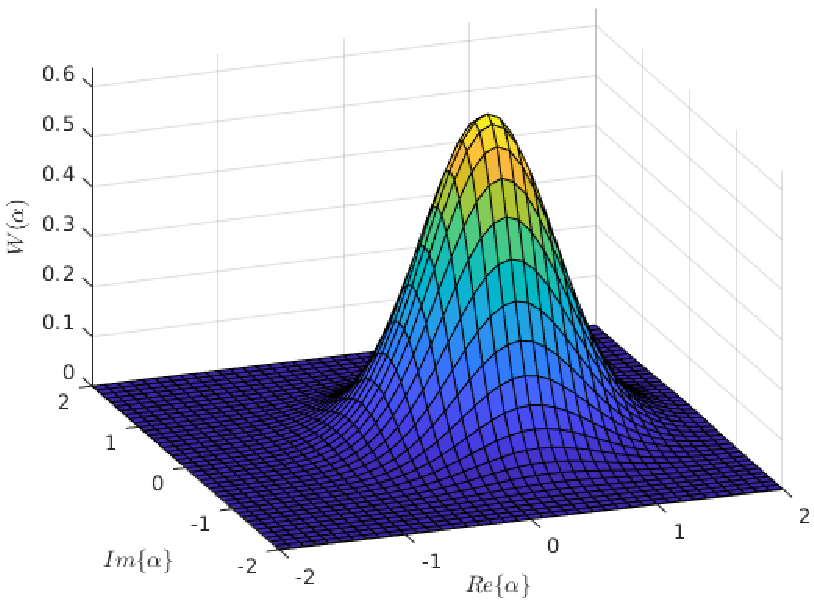
\includegraphics[width=\linewidth]{Pictures/WigCohState.pdf}
                    % This file was created by matlab2tikz.
%
%The latest updates can be retrieved from
%  http://www.mathworks.com/matlabcentral/fileexchange/22022-matlab2tikz-matlab2tikz
%where you can also make suggestions and rate matlab2tikz.
%
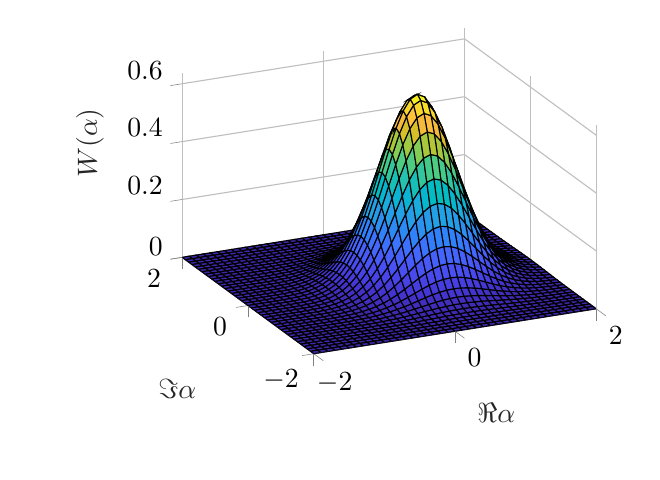
\begin{tikzpicture}

\begin{axis}[%
width=4.602in*0.45,
height=3.617in*0.45,
at={(0.772in,0.488in)},
scale only axis,
xmin=-2,
xmax=2,
tick align=outside,
xlabel style={font=\color{white!15!black}},
xlabel={$\Re{ \alpha }$},
ymin=-2,
ymax=2,
ylabel style={font=\color{white!15!black}},
ylabel={$\Im{ \alpha }$},
zmin=0,
zmax=0.636619772367581,
zlabel style={font=\color{white!15!black}},
zlabel={$W( \alpha )$},
view={-25}{30},
axis background/.style={fill=white},
axis x line*=bottom,
axis y line*=left,
axis z line*=left,
xmajorgrids,
ymajorgrids,
zmajorgrids
]

\addplot3[%
surf,
shader=flat corner, draw=black, z buffer=sort, colormap={mymap}{[1pt] rgb(0pt)=(0.2422,0.1504,0.6603); rgb(1pt)=(0.2444,0.1534,0.6728); rgb(2pt)=(0.2464,0.1569,0.6847); rgb(3pt)=(0.2484,0.1607,0.6961); rgb(4pt)=(0.2503,0.1648,0.7071); rgb(5pt)=(0.2522,0.1689,0.7179); rgb(6pt)=(0.254,0.1732,0.7286); rgb(7pt)=(0.2558,0.1773,0.7393); rgb(8pt)=(0.2576,0.1814,0.7501); rgb(9pt)=(0.2594,0.1854,0.761); rgb(11pt)=(0.2628,0.1932,0.7828); rgb(12pt)=(0.2645,0.1972,0.7937); rgb(13pt)=(0.2661,0.2011,0.8043); rgb(14pt)=(0.2676,0.2052,0.8148); rgb(15pt)=(0.2691,0.2094,0.8249); rgb(16pt)=(0.2704,0.2138,0.8346); rgb(17pt)=(0.2717,0.2184,0.8439); rgb(18pt)=(0.2729,0.2231,0.8528); rgb(19pt)=(0.274,0.228,0.8612); rgb(20pt)=(0.2749,0.233,0.8692); rgb(21pt)=(0.2758,0.2382,0.8767); rgb(22pt)=(0.2766,0.2435,0.884); rgb(23pt)=(0.2774,0.2489,0.8908); rgb(24pt)=(0.2781,0.2543,0.8973); rgb(25pt)=(0.2788,0.2598,0.9035); rgb(26pt)=(0.2794,0.2653,0.9094); rgb(27pt)=(0.2798,0.2708,0.915); rgb(28pt)=(0.2802,0.2764,0.9204); rgb(29pt)=(0.2806,0.2819,0.9255); rgb(30pt)=(0.2809,0.2875,0.9305); rgb(31pt)=(0.2811,0.293,0.9352); rgb(32pt)=(0.2813,0.2985,0.9397); rgb(33pt)=(0.2814,0.304,0.9441); rgb(34pt)=(0.2814,0.3095,0.9483); rgb(35pt)=(0.2813,0.315,0.9524); rgb(36pt)=(0.2811,0.3204,0.9563); rgb(37pt)=(0.2809,0.3259,0.96); rgb(38pt)=(0.2807,0.3313,0.9636); rgb(39pt)=(0.2803,0.3367,0.967); rgb(40pt)=(0.2798,0.3421,0.9702); rgb(41pt)=(0.2791,0.3475,0.9733); rgb(42pt)=(0.2784,0.3529,0.9763); rgb(43pt)=(0.2776,0.3583,0.9791); rgb(44pt)=(0.2766,0.3638,0.9817); rgb(45pt)=(0.2754,0.3693,0.984); rgb(46pt)=(0.2741,0.3748,0.9862); rgb(47pt)=(0.2726,0.3804,0.9881); rgb(48pt)=(0.271,0.386,0.9898); rgb(49pt)=(0.2691,0.3916,0.9912); rgb(50pt)=(0.267,0.3973,0.9924); rgb(51pt)=(0.2647,0.403,0.9935); rgb(52pt)=(0.2621,0.4088,0.9946); rgb(53pt)=(0.2591,0.4145,0.9955); rgb(54pt)=(0.2556,0.4203,0.9965); rgb(55pt)=(0.2517,0.4261,0.9974); rgb(56pt)=(0.2473,0.4319,0.9983); rgb(57pt)=(0.2424,0.4378,0.9991); rgb(58pt)=(0.2369,0.4437,0.9996); rgb(59pt)=(0.2311,0.4497,0.9995); rgb(60pt)=(0.225,0.4559,0.9985); rgb(61pt)=(0.2189,0.462,0.9968); rgb(62pt)=(0.2128,0.4682,0.9948); rgb(63pt)=(0.2066,0.4743,0.9926); rgb(64pt)=(0.2006,0.4803,0.9906); rgb(65pt)=(0.195,0.4861,0.9887); rgb(66pt)=(0.1903,0.4919,0.9867); rgb(67pt)=(0.1869,0.4975,0.9844); rgb(68pt)=(0.1847,0.503,0.9819); rgb(69pt)=(0.1831,0.5084,0.9793); rgb(70pt)=(0.1818,0.5138,0.9766); rgb(71pt)=(0.1806,0.5191,0.9738); rgb(72pt)=(0.1795,0.5244,0.9709); rgb(73pt)=(0.1785,0.5296,0.9677); rgb(74pt)=(0.1778,0.5349,0.9641); rgb(75pt)=(0.1773,0.5401,0.9602); rgb(76pt)=(0.1768,0.5452,0.956); rgb(77pt)=(0.1764,0.5504,0.9516); rgb(78pt)=(0.1755,0.5554,0.9473); rgb(79pt)=(0.174,0.5605,0.9432); rgb(80pt)=(0.1716,0.5655,0.9393); rgb(81pt)=(0.1686,0.5705,0.9357); rgb(82pt)=(0.1649,0.5755,0.9323); rgb(83pt)=(0.161,0.5805,0.9289); rgb(84pt)=(0.1573,0.5854,0.9254); rgb(85pt)=(0.154,0.5902,0.9218); rgb(86pt)=(0.1513,0.595,0.9182); rgb(87pt)=(0.1492,0.5997,0.9147); rgb(88pt)=(0.1475,0.6043,0.9113); rgb(89pt)=(0.1461,0.6089,0.908); rgb(90pt)=(0.1446,0.6135,0.905); rgb(91pt)=(0.1429,0.618,0.9022); rgb(92pt)=(0.1408,0.6226,0.8998); rgb(93pt)=(0.1383,0.6272,0.8975); rgb(94pt)=(0.1354,0.6317,0.8953); rgb(95pt)=(0.1321,0.6363,0.8932); rgb(96pt)=(0.1288,0.6408,0.891); rgb(97pt)=(0.1253,0.6453,0.8887); rgb(98pt)=(0.1219,0.6497,0.8862); rgb(99pt)=(0.1185,0.6541,0.8834); rgb(100pt)=(0.1152,0.6584,0.8804); rgb(101pt)=(0.1119,0.6627,0.877); rgb(102pt)=(0.1085,0.6669,0.8734); rgb(103pt)=(0.1048,0.671,0.8695); rgb(104pt)=(0.1009,0.675,0.8653); rgb(105pt)=(0.0964,0.6789,0.8609); rgb(106pt)=(0.0914,0.6828,0.8562); rgb(107pt)=(0.0855,0.6865,0.8513); rgb(108pt)=(0.0789,0.6902,0.8462); rgb(109pt)=(0.0713,0.6938,0.8409); rgb(110pt)=(0.0628,0.6972,0.8355); rgb(111pt)=(0.0535,0.7006,0.8299); rgb(112pt)=(0.0433,0.7039,0.8242); rgb(113pt)=(0.0328,0.7071,0.8183); rgb(114pt)=(0.0234,0.7103,0.8124); rgb(115pt)=(0.0155,0.7133,0.8064); rgb(116pt)=(0.0091,0.7163,0.8003); rgb(117pt)=(0.0046,0.7192,0.7941); rgb(118pt)=(0.0019,0.722,0.7878); rgb(119pt)=(0.0009,0.7248,0.7815); rgb(120pt)=(0.0018,0.7275,0.7752); rgb(121pt)=(0.0046,0.7301,0.7688); rgb(122pt)=(0.0094,0.7327,0.7623); rgb(123pt)=(0.0162,0.7352,0.7558); rgb(124pt)=(0.0253,0.7376,0.7492); rgb(125pt)=(0.0369,0.74,0.7426); rgb(126pt)=(0.0504,0.7423,0.7359); rgb(127pt)=(0.0638,0.7446,0.7292); rgb(128pt)=(0.077,0.7468,0.7224); rgb(129pt)=(0.0899,0.7489,0.7156); rgb(130pt)=(0.1023,0.751,0.7088); rgb(131pt)=(0.1141,0.7531,0.7019); rgb(132pt)=(0.1252,0.7552,0.695); rgb(133pt)=(0.1354,0.7572,0.6881); rgb(134pt)=(0.1448,0.7593,0.6812); rgb(135pt)=(0.1532,0.7614,0.6741); rgb(136pt)=(0.1609,0.7635,0.6671); rgb(137pt)=(0.1678,0.7656,0.6599); rgb(138pt)=(0.1741,0.7678,0.6527); rgb(139pt)=(0.1799,0.7699,0.6454); rgb(140pt)=(0.1853,0.7721,0.6379); rgb(141pt)=(0.1905,0.7743,0.6303); rgb(142pt)=(0.1954,0.7765,0.6225); rgb(143pt)=(0.2003,0.7787,0.6146); rgb(144pt)=(0.2061,0.7808,0.6065); rgb(145pt)=(0.2118,0.7828,0.5983); rgb(146pt)=(0.2178,0.7849,0.5899); rgb(147pt)=(0.2244,0.7869,0.5813); rgb(148pt)=(0.2318,0.7887,0.5725); rgb(149pt)=(0.2401,0.7905,0.5636); rgb(150pt)=(0.2491,0.7922,0.5546); rgb(151pt)=(0.2589,0.7937,0.5454); rgb(152pt)=(0.2695,0.7951,0.536); rgb(153pt)=(0.2809,0.7964,0.5266); rgb(154pt)=(0.2929,0.7975,0.517); rgb(155pt)=(0.3052,0.7985,0.5074); rgb(156pt)=(0.3176,0.7994,0.4975); rgb(157pt)=(0.3301,0.8002,0.4876); rgb(158pt)=(0.3424,0.8009,0.4774); rgb(159pt)=(0.3548,0.8016,0.4669); rgb(160pt)=(0.3671,0.8021,0.4563); rgb(161pt)=(0.3795,0.8026,0.4454); rgb(162pt)=(0.3921,0.8029,0.4344); rgb(163pt)=(0.405,0.8031,0.4233); rgb(164pt)=(0.4184,0.803,0.4122); rgb(165pt)=(0.4322,0.8028,0.4013); rgb(166pt)=(0.4463,0.8024,0.3904); rgb(167pt)=(0.4608,0.8018,0.3797); rgb(168pt)=(0.4753,0.8011,0.3691); rgb(169pt)=(0.4899,0.8002,0.3586); rgb(170pt)=(0.5044,0.7993,0.348); rgb(171pt)=(0.5187,0.7982,0.3374); rgb(172pt)=(0.5329,0.797,0.3267); rgb(173pt)=(0.547,0.7957,0.3159); rgb(175pt)=(0.5748,0.7929,0.2941); rgb(176pt)=(0.5886,0.7913,0.2833); rgb(177pt)=(0.6024,0.7896,0.2726); rgb(178pt)=(0.6161,0.7878,0.2622); rgb(179pt)=(0.6297,0.7859,0.2521); rgb(180pt)=(0.6433,0.7839,0.2423); rgb(181pt)=(0.6567,0.7818,0.2329); rgb(182pt)=(0.6701,0.7796,0.2239); rgb(183pt)=(0.6833,0.7773,0.2155); rgb(184pt)=(0.6963,0.775,0.2075); rgb(185pt)=(0.7091,0.7727,0.1998); rgb(186pt)=(0.7218,0.7703,0.1924); rgb(187pt)=(0.7344,0.7679,0.1852); rgb(188pt)=(0.7468,0.7654,0.1782); rgb(189pt)=(0.759,0.7629,0.1717); rgb(190pt)=(0.771,0.7604,0.1658); rgb(191pt)=(0.7829,0.7579,0.1608); rgb(192pt)=(0.7945,0.7554,0.157); rgb(193pt)=(0.806,0.7529,0.1546); rgb(194pt)=(0.8172,0.7505,0.1535); rgb(195pt)=(0.8281,0.7481,0.1536); rgb(196pt)=(0.8389,0.7457,0.1546); rgb(197pt)=(0.8495,0.7435,0.1564); rgb(198pt)=(0.86,0.7413,0.1587); rgb(199pt)=(0.8703,0.7392,0.1615); rgb(200pt)=(0.8804,0.7372,0.165); rgb(201pt)=(0.8903,0.7353,0.1695); rgb(202pt)=(0.9,0.7336,0.1749); rgb(203pt)=(0.9093,0.7321,0.1815); rgb(204pt)=(0.9184,0.7308,0.189); rgb(205pt)=(0.9272,0.7298,0.1973); rgb(206pt)=(0.9357,0.729,0.2061); rgb(207pt)=(0.944,0.7285,0.2151); rgb(208pt)=(0.9523,0.7284,0.2237); rgb(209pt)=(0.9606,0.7285,0.2312); rgb(210pt)=(0.9689,0.7292,0.2373); rgb(211pt)=(0.977,0.7304,0.2418); rgb(212pt)=(0.9842,0.733,0.2446); rgb(213pt)=(0.99,0.7365,0.2429); rgb(214pt)=(0.9946,0.7407,0.2394); rgb(215pt)=(0.9966,0.7458,0.2351); rgb(216pt)=(0.9971,0.7513,0.2309); rgb(217pt)=(0.9972,0.7569,0.2267); rgb(218pt)=(0.9971,0.7626,0.2224); rgb(219pt)=(0.9969,0.7683,0.2181); rgb(220pt)=(0.9966,0.774,0.2138); rgb(221pt)=(0.9962,0.7798,0.2095); rgb(222pt)=(0.9957,0.7856,0.2053); rgb(223pt)=(0.9949,0.7915,0.2012); rgb(224pt)=(0.9938,0.7974,0.1974); rgb(225pt)=(0.9923,0.8034,0.1939); rgb(226pt)=(0.9906,0.8095,0.1906); rgb(227pt)=(0.9885,0.8156,0.1875); rgb(228pt)=(0.9861,0.8218,0.1846); rgb(229pt)=(0.9835,0.828,0.1817); rgb(230pt)=(0.9807,0.8342,0.1787); rgb(231pt)=(0.9778,0.8404,0.1757); rgb(232pt)=(0.9748,0.8467,0.1726); rgb(233pt)=(0.972,0.8529,0.1695); rgb(234pt)=(0.9694,0.8591,0.1665); rgb(235pt)=(0.9671,0.8654,0.1636); rgb(236pt)=(0.9651,0.8716,0.1608); rgb(237pt)=(0.9634,0.8778,0.1582); rgb(238pt)=(0.9619,0.884,0.1557); rgb(239pt)=(0.9608,0.8902,0.1532); rgb(240pt)=(0.9601,0.8963,0.1507); rgb(241pt)=(0.9596,0.9023,0.148); rgb(242pt)=(0.9595,0.9084,0.145); rgb(243pt)=(0.9597,0.9143,0.1418); rgb(244pt)=(0.9601,0.9203,0.1382); rgb(245pt)=(0.9608,0.9262,0.1344); rgb(246pt)=(0.9618,0.932,0.1304); rgb(247pt)=(0.9629,0.9379,0.1261); rgb(248pt)=(0.9642,0.9437,0.1216); rgb(249pt)=(0.9657,0.9494,0.1168); rgb(250pt)=(0.9674,0.9552,0.1116); rgb(251pt)=(0.9692,0.9609,0.1061); rgb(252pt)=(0.9711,0.9667,0.1001); rgb(253pt)=(0.973,0.9724,0.0938); rgb(254pt)=(0.9749,0.9782,0.0872); rgb(255pt)=(0.9769,0.9839,0.0805)}, mesh/rows=41]
table[row sep=crcr, point meta=\thisrow{c}] {%
%
x	y	z	c\\
-2	-2	2.12056620670023e-09	2.12056620670023e-09\\
-2	-1.9	4.62595636706929e-09	4.62595636706929e-09\\
-2	-1.8	9.69570623824183e-09	9.69570623824183e-09\\
-2	-1.7	1.95247546880979e-08	1.95247546880979e-08\\
-2	-1.6	3.77763457016117e-08	3.77763457016117e-08\\
-2	-1.5	7.02235083432076e-08	7.02235083432076e-08\\
-2	-1.4	1.25421884643068e-07	1.25421884643068e-07\\
-2	-1.3	2.15224814715663e-07	2.15224814715663e-07\\
-2	-1.2	3.54845730004206e-07	3.54845730004206e-07\\
-2	-1.1	5.62101889586039e-07	5.62101889586039e-07\\
-2	-1	8.55497466290539e-07	8.55497466290539e-07\\
-2	-0.9	1.25098076125668e-06	1.25098076125668e-06\\
-2	-0.8	1.75756240636898e-06	1.75756240636898e-06\\
-2	-0.7	2.37246109410165e-06	2.37246109410165e-06\\
-2	-0.6	3.07691617238443e-06	3.07691617238443e-06\\
-2	-0.5	3.83407364437623e-06	3.83407364437623e-06\\
-2	-0.4	4.59021953853494e-06	4.59021953853494e-06\\
-2	-0.3	5.28000926617924e-06	5.28000926617924e-06\\
-2	-0.2	5.83531268815123e-06	5.83531268815123e-06\\
-2	-0.0999999999999999	6.19614827279883e-06	6.19614827279883e-06\\
-2	0	6.32131877091383e-06	6.32131877091383e-06\\
-2	0.0999999999999999	6.19614827279883e-06	6.19614827279883e-06\\
-2	0.2	5.83531268815123e-06	5.83531268815123e-06\\
-2	0.3	5.28000926617924e-06	5.28000926617924e-06\\
-2	0.4	4.59021953853494e-06	4.59021953853494e-06\\
-2	0.5	3.83407364437623e-06	3.83407364437623e-06\\
-2	0.6	3.07691617238443e-06	3.07691617238443e-06\\
-2	0.7	2.37246109410165e-06	2.37246109410165e-06\\
-2	0.8	1.75756240636898e-06	1.75756240636898e-06\\
-2	0.9	1.25098076125668e-06	1.25098076125668e-06\\
-2	1	8.55497466290539e-07	8.55497466290539e-07\\
-2	1.1	5.62101889586039e-07	5.62101889586039e-07\\
-2	1.2	3.54845730004206e-07	3.54845730004206e-07\\
-2	1.3	2.15224814715663e-07	2.15224814715663e-07\\
-2	1.4	1.25421884643068e-07	1.25421884643068e-07\\
-2	1.5	7.02235083432076e-08	7.02235083432076e-08\\
-2	1.6	3.77763457016117e-08	3.77763457016117e-08\\
-2	1.7	1.95247546880979e-08	1.95247546880979e-08\\
-2	1.8	9.69570623824183e-09	9.69570623824183e-09\\
-2	1.9	4.62595636706929e-09	4.62595636706929e-09\\
-2	2	2.12056620670023e-09	2.12056620670023e-09\\
-1.9	-2	5.42861008548959e-09	5.42861008548959e-09\\
-1.9	-1.9	1.18423623416994e-08	1.18423623416994e-08\\
-1.9	-1.8	2.48208278074783e-08	2.48208278074783e-08\\
-1.9	-1.7	4.99830091989677e-08	4.99830091989677e-08\\
-1.9	-1.6	9.67067430485095e-08	9.67067430485095e-08\\
-1.9	-1.5	1.79770876488503e-07	1.79770876488503e-07\\
-1.9	-1.4	3.21077694138091e-07	3.21077694138091e-07\\
-1.9	-1.3	5.50971526435457e-07	5.50971526435457e-07\\
-1.9	-1.2	9.08398475184253e-07	9.08398475184253e-07\\
-1.9	-1.1	1.43897039254803e-06	1.43897039254803e-06\\
-1.9	-1	2.19005761713156e-06	2.19005761713156e-06\\
-1.9	-0.9	3.20248750350451e-06	3.20248750350451e-06\\
-1.9	-0.8	4.49932710185868e-06	4.49932710185868e-06\\
-1.9	-0.7	6.07345631660937e-06	6.07345631660937e-06\\
-1.9	-0.6	7.87684822706097e-06	7.87684822706097e-06\\
-1.9	-0.5	9.81515728610915e-06	9.81515728610915e-06\\
-1.9	-0.4	1.17508767247014e-05	1.17508767247014e-05\\
-1.9	-0.3	1.35167256100252e-05	1.35167256100252e-05\\
-1.9	-0.2	1.49382920518082e-05	1.49382920518082e-05\\
-1.9	-0.0999999999999999	1.5862024443578e-05	1.5862024443578e-05\\
-1.9	0	1.61824585928755e-05	1.61824585928755e-05\\
-1.9	0.0999999999999999	1.5862024443578e-05	1.5862024443578e-05\\
-1.9	0.2	1.49382920518082e-05	1.49382920518082e-05\\
-1.9	0.3	1.35167256100252e-05	1.35167256100252e-05\\
-1.9	0.4	1.17508767247014e-05	1.17508767247014e-05\\
-1.9	0.5	9.81515728610915e-06	9.81515728610915e-06\\
-1.9	0.6	7.87684822706097e-06	7.87684822706097e-06\\
-1.9	0.7	6.07345631660937e-06	6.07345631660937e-06\\
-1.9	0.8	4.49932710185868e-06	4.49932710185868e-06\\
-1.9	0.9	3.20248750350451e-06	3.20248750350451e-06\\
-1.9	1	2.19005761713156e-06	2.19005761713156e-06\\
-1.9	1.1	1.43897039254803e-06	1.43897039254803e-06\\
-1.9	1.2	9.08398475184253e-07	9.08398475184253e-07\\
-1.9	1.3	5.50971526435457e-07	5.50971526435457e-07\\
-1.9	1.4	3.21077694138091e-07	3.21077694138091e-07\\
-1.9	1.5	1.79770876488503e-07	1.79770876488503e-07\\
-1.9	1.6	9.67067430485095e-08	9.67067430485095e-08\\
-1.9	1.7	4.99830091989677e-08	4.99830091989677e-08\\
-1.9	1.8	2.48208278074783e-08	2.48208278074783e-08\\
-1.9	1.9	1.18423623416994e-08	1.18423623416994e-08\\
-1.9	2	5.42861008548959e-09	5.42861008548959e-09\\
-1.8	-2	1.33522262555282e-08	1.33522262555282e-08\\
-1.8	-1.9	2.91275112590915e-08	2.91275112590915e-08\\
-1.8	-1.8	6.10493852967643e-08	6.10493852967643e-08\\
-1.8	-1.7	1.22938364930768e-07	1.22938364930768e-07\\
-1.8	-1.6	2.37860206071969e-07	2.37860206071969e-07\\
-1.8	-1.5	4.42165007106532e-07	4.42165007106532e-07\\
-1.8	-1.4	7.89723695425148e-07	7.89723695425148e-07\\
-1.8	-1.3	1.35517128057954e-06	1.35517128057954e-06\\
-1.8	-1.2	2.23429971573341e-06	2.23429971573341e-06\\
-1.8	-1.1	3.53929605437386e-06	3.53929605437386e-06\\
-1.8	-1	5.38667252870974e-06	5.38667252870974e-06\\
-1.8	-0.9	7.87684822706094e-06	7.87684822706094e-06\\
-1.8	-0.8	1.10665589378444e-05	1.10665589378444e-05\\
-1.8	-0.7	1.49382920518082e-05	1.49382920518082e-05\\
-1.8	-0.6	1.93739204053902e-05	1.93739204053902e-05\\
-1.8	-0.5	2.41413913974088e-05	2.41413913974088e-05\\
-1.8	-0.4	2.89024929508972e-05	2.89024929508972e-05\\
-1.8	-0.3	3.32457803630728e-05	3.32457803630728e-05\\
-1.8	-0.2	3.67422696059986e-05	3.67422696059986e-05\\
-1.8	-0.0999999999999999	3.9014284670672e-05	3.9014284670672e-05\\
-1.8	0	3.98024255012049e-05	3.98024255012049e-05\\
-1.8	0.0999999999999999	3.9014284670672e-05	3.9014284670672e-05\\
-1.8	0.2	3.67422696059986e-05	3.67422696059986e-05\\
-1.8	0.3	3.32457803630728e-05	3.32457803630728e-05\\
-1.8	0.4	2.89024929508972e-05	2.89024929508972e-05\\
-1.8	0.5	2.41413913974088e-05	2.41413913974088e-05\\
-1.8	0.6	1.93739204053902e-05	1.93739204053902e-05\\
-1.8	0.7	1.49382920518082e-05	1.49382920518082e-05\\
-1.8	0.8	1.10665589378444e-05	1.10665589378444e-05\\
-1.8	0.9	7.87684822706094e-06	7.87684822706094e-06\\
-1.8	1	5.38667252870974e-06	5.38667252870974e-06\\
-1.8	1.1	3.53929605437386e-06	3.53929605437386e-06\\
-1.8	1.2	2.23429971573341e-06	2.23429971573341e-06\\
-1.8	1.3	1.35517128057954e-06	1.35517128057954e-06\\
-1.8	1.4	7.89723695425148e-07	7.89723695425148e-07\\
-1.8	1.5	4.42165007106532e-07	4.42165007106532e-07\\
-1.8	1.6	2.37860206071969e-07	2.37860206071969e-07\\
-1.8	1.7	1.22938364930768e-07	1.22938364930768e-07\\
-1.8	1.8	6.10493852967643e-08	6.10493852967643e-08\\
-1.8	1.9	2.91275112590915e-08	2.91275112590915e-08\\
-1.8	2	1.33522262555282e-08	1.33522262555282e-08\\
-1.7	-2	3.15534562605306e-08	3.15534562605306e-08\\
-1.7	-1.9	6.88329897129583e-08	6.88329897129583e-08\\
-1.7	-1.8	1.44269507708214e-07	1.44269507708214e-07\\
-1.7	-1.7	2.9052311175285e-07	2.9052311175285e-07\\
-1.7	-1.6	5.62101889586037e-07	5.62101889586037e-07\\
-1.7	-1.5	1.0449069649263e-06	1.0449069649263e-06\\
-1.7	-1.4	1.86624399591679e-06	1.86624399591679e-06\\
-1.7	-1.3	3.20248750350451e-06	3.20248750350451e-06\\
-1.7	-1.2	5.28000926617922e-06	5.28000926617922e-06\\
-1.7	-1.1	8.36392531908433e-06	8.36392531908433e-06\\
-1.7	-1	1.27295727897117e-05	1.27295727897117e-05\\
-1.7	-0.9	1.86142581204766e-05	1.86142581204766e-05\\
-1.7	-0.8	2.61520570964924e-05	2.61520570964924e-05\\
-1.7	-0.7	3.53015846079308e-05	3.53015846079308e-05\\
-1.7	-0.6	4.57836871850027e-05	4.57836871850027e-05\\
-1.7	-0.5	5.70499872417235e-05	5.70499872417235e-05\\
-1.7	-0.4	6.83012352916692e-05	6.83012352916692e-05\\
-1.7	-0.3	7.85651213855899e-05	7.85651213855899e-05\\
-1.7	-0.2	8.6827887330437e-05	8.6827887330437e-05\\
-1.7	-0.0999999999999999	9.21970240267807e-05	9.21970240267807e-05\\
-1.7	0	9.40595274586007e-05	9.40595274586007e-05\\
-1.7	0.0999999999999999	9.21970240267807e-05	9.21970240267807e-05\\
-1.7	0.2	8.6827887330437e-05	8.6827887330437e-05\\
-1.7	0.3	7.85651213855899e-05	7.85651213855899e-05\\
-1.7	0.4	6.83012352916692e-05	6.83012352916692e-05\\
-1.7	0.5	5.70499872417235e-05	5.70499872417235e-05\\
-1.7	0.6	4.57836871850027e-05	4.57836871850027e-05\\
-1.7	0.7	3.53015846079308e-05	3.53015846079308e-05\\
-1.7	0.8	2.61520570964924e-05	2.61520570964924e-05\\
-1.7	0.9	1.86142581204766e-05	1.86142581204766e-05\\
-1.7	1	1.27295727897117e-05	1.27295727897117e-05\\
-1.7	1.1	8.36392531908433e-06	8.36392531908433e-06\\
-1.7	1.2	5.28000926617922e-06	5.28000926617922e-06\\
-1.7	1.3	3.20248750350451e-06	3.20248750350451e-06\\
-1.7	1.4	1.86624399591679e-06	1.86624399591679e-06\\
-1.7	1.5	1.0449069649263e-06	1.0449069649263e-06\\
-1.7	1.6	5.62101889586037e-07	5.62101889586037e-07\\
-1.7	1.7	2.9052311175285e-07	2.9052311175285e-07\\
-1.7	1.8	1.44269507708214e-07	1.44269507708214e-07\\
-1.7	1.9	6.88329897129583e-08	6.88329897129583e-08\\
-1.7	2	3.15534562605306e-08	3.15534562605306e-08\\
-1.6	-2	7.16421173131205e-08	7.16421173131205e-08\\
-1.6	-1.9	1.56285291960142e-07	1.56285291960142e-07\\
-1.6	-1.8	3.2756389381238e-07	3.2756389381238e-07\\
-1.6	-1.7	6.59632678034255e-07	6.59632678034255e-07\\
-1.6	-1.6	1.27625224898176e-06	1.27625224898176e-06\\
-1.6	-1.5	2.37246109410165e-06	2.37246109410165e-06\\
-1.6	-1.4	4.23730668952491e-06	4.23730668952491e-06\\
-1.6	-1.3	7.27124735640655e-06	7.27124735640655e-06\\
-1.6	-1.2	1.19882601810296e-05	1.19882601810296e-05\\
-1.6	-1.1	1.89902910781142e-05	1.89902910781142e-05\\
-1.6	-1	2.89024929508972e-05	2.89024929508972e-05\\
-1.6	-0.9	4.22636700383285e-05	4.22636700383285e-05\\
-1.6	-0.8	5.93782413887243e-05	5.93782413887243e-05\\
-1.6	-0.7	8.01522421169434e-05	8.01522421169434e-05\\
-1.6	-0.6	0.000103951854315184	0.000103951854315184\\
-1.6	-0.5	0.000129531986763559	0.000129531986763559\\
-1.6	-0.4	0.000155077943632998	0.000155077943632998\\
-1.6	-0.3	0.000178382095341695	0.000178382095341695\\
-1.6	-0.2	0.000197142704077039	0.000197142704077039\\
-1.6	-0.0999999999999999	0.000209333328073777	0.000209333328073777\\
-1.6	0	0.000213562141813128	0.000213562141813128\\
-1.6	0.0999999999999999	0.000209333328073777	0.000209333328073777\\
-1.6	0.2	0.000197142704077039	0.000197142704077039\\
-1.6	0.3	0.000178382095341695	0.000178382095341695\\
-1.6	0.4	0.000155077943632998	0.000155077943632998\\
-1.6	0.5	0.000129531986763559	0.000129531986763559\\
-1.6	0.6	0.000103951854315184	0.000103951854315184\\
-1.6	0.7	8.01522421169434e-05	8.01522421169434e-05\\
-1.6	0.8	5.93782413887243e-05	5.93782413887243e-05\\
-1.6	0.9	4.22636700383285e-05	4.22636700383285e-05\\
-1.6	1	2.89024929508972e-05	2.89024929508972e-05\\
-1.6	1.1	1.89902910781142e-05	1.89902910781142e-05\\
-1.6	1.2	1.19882601810296e-05	1.19882601810296e-05\\
-1.6	1.3	7.27124735640655e-06	7.27124735640655e-06\\
-1.6	1.4	4.23730668952491e-06	4.23730668952491e-06\\
-1.6	1.5	2.37246109410165e-06	2.37246109410165e-06\\
-1.6	1.6	1.27625224898176e-06	1.27625224898176e-06\\
-1.6	1.7	6.59632678034255e-07	6.59632678034255e-07\\
-1.6	1.8	3.2756389381238e-07	3.2756389381238e-07\\
-1.6	1.9	1.56285291960142e-07	1.56285291960142e-07\\
-1.6	2	7.16421173131205e-08	7.16421173131205e-08\\
-1.5	-2	1.56285291960142e-07	1.56285291960142e-07\\
-1.5	-1.9	3.40932029916338e-07	3.40932029916338e-07\\
-1.5	-1.8	7.14571549530306e-07	7.14571549530306e-07\\
-1.5	-1.7	1.43897039254803e-06	1.43897039254803e-06\\
-1.5	-1.6	2.78410888493341e-06	2.78410888493341e-06\\
-1.5	-1.5	5.17545807775626e-06	5.17545807775626e-06\\
-1.5	-1.4	9.2435670236086e-06	9.2435670236086e-06\\
-1.5	-1.3	1.5862024443578e-05	1.5862024443578e-05\\
-1.5	-1.2	2.61520570964924e-05	2.61520570964924e-05\\
-1.5	-1.1	4.1426793300644e-05	4.1426793300644e-05\\
-1.5	-1	6.30499867761398e-05	6.30499867761398e-05\\
-1.5	-0.9	9.21970240267807e-05	9.21970240267807e-05\\
-1.5	-0.8	0.00012953198676356	0.00012953198676356\\
-1.5	-0.7	0.000174849893195609	0.000174849893195609\\
-1.5	-0.6	0.000226768087135682	0.000226768087135682\\
-1.5	-0.5	0.000282570436619585	0.000282570436619585\\
-1.5	-0.4	0.000338298233025878	0.000338298233025878\\
-1.5	-0.3	0.000389135593649365	0.000389135593649365\\
-1.5	-0.2	0.00043006134128938	0.00043006134128938\\
-1.5	-0.0999999999999999	0.000456654849437381	0.000456654849437381\\
-1.5	0	0.000465879889325732	0.000465879889325732\\
-1.5	0.0999999999999999	0.000456654849437381	0.000456654849437381\\
-1.5	0.2	0.00043006134128938	0.00043006134128938\\
-1.5	0.3	0.000389135593649365	0.000389135593649365\\
-1.5	0.4	0.000338298233025878	0.000338298233025878\\
-1.5	0.5	0.000282570436619585	0.000282570436619585\\
-1.5	0.6	0.000226768087135682	0.000226768087135682\\
-1.5	0.7	0.000174849893195609	0.000174849893195609\\
-1.5	0.8	0.00012953198676356	0.00012953198676356\\
-1.5	0.9	9.21970240267807e-05	9.21970240267807e-05\\
-1.5	1	6.30499867761398e-05	6.30499867761398e-05\\
-1.5	1.1	4.1426793300644e-05	4.1426793300644e-05\\
-1.5	1.2	2.61520570964924e-05	2.61520570964924e-05\\
-1.5	1.3	1.5862024443578e-05	1.5862024443578e-05\\
-1.5	1.4	9.2435670236086e-06	9.2435670236086e-06\\
-1.5	1.5	5.17545807775626e-06	5.17545807775626e-06\\
-1.5	1.6	2.78410888493341e-06	2.78410888493341e-06\\
-1.5	1.7	1.43897039254803e-06	1.43897039254803e-06\\
-1.5	1.8	7.14571549530306e-07	7.14571549530306e-07\\
-1.5	1.9	3.40932029916338e-07	3.40932029916338e-07\\
-1.5	2	1.56285291960142e-07	1.56285291960142e-07\\
-1.4	-2	3.27563893812382e-07	3.27563893812382e-07\\
-1.4	-1.9	7.14571549530309e-07	7.14571549530309e-07\\
-1.4	-1.8	1.49769588830784e-06	1.49769588830784e-06\\
-1.4	-1.7	3.01598915004732e-06	3.01598915004732e-06\\
-1.4	-1.6	5.83531268815123e-06	5.83531268815123e-06\\
-1.4	-1.5	1.08474263889461e-05	1.08474263889461e-05\\
-1.4	-1.4	1.93739204053903e-05	1.93739204053903e-05\\
-1.4	-1.3	3.32457803630729e-05	3.32457803630729e-05\\
-1.4	-1.2	5.4813025245623e-05	5.4813025245623e-05\\
-1.4	-1.1	8.6827887330437e-05	8.6827887330437e-05\\
-1.4	-1	0.000132148706472511	0.000132148706472511\\
-1.4	-0.9	0.00019323901698842	0.00019323901698842\\
-1.4	-0.8	0.000271490691320759	0.000271490691320759\\
-1.4	-0.7	0.000366474100854223	0.000366474100854223\\
-1.4	-0.6	0.00047529128738163	0.00047529128738163\\
-1.4	-0.5	0.000592249413457167	0.000592249413457167\\
-1.4	-0.4	0.000709051281089629	0.000709051281089629\\
-1.4	-0.3	0.000815603110683551	0.000815603110683551\\
-1.4	-0.2	0.000901380838619493	0.000901380838619493\\
-1.4	-0.0999999999999999	0.000957119116801884	0.000957119116801884\\
-1.4	0	0.000976454205526507	0.000976454205526507\\
-1.4	0.0999999999999999	0.000957119116801884	0.000957119116801884\\
-1.4	0.2	0.000901380838619493	0.000901380838619493\\
-1.4	0.3	0.000815603110683551	0.000815603110683551\\
-1.4	0.4	0.000709051281089629	0.000709051281089629\\
-1.4	0.5	0.000592249413457167	0.000592249413457167\\
-1.4	0.6	0.00047529128738163	0.00047529128738163\\
-1.4	0.7	0.000366474100854223	0.000366474100854223\\
-1.4	0.8	0.000271490691320759	0.000271490691320759\\
-1.4	0.9	0.00019323901698842	0.00019323901698842\\
-1.4	1	0.000132148706472511	0.000132148706472511\\
-1.4	1.1	8.6827887330437e-05	8.6827887330437e-05\\
-1.4	1.2	5.4813025245623e-05	5.4813025245623e-05\\
-1.4	1.3	3.32457803630729e-05	3.32457803630729e-05\\
-1.4	1.4	1.93739204053903e-05	1.93739204053903e-05\\
-1.4	1.5	1.08474263889461e-05	1.08474263889461e-05\\
-1.4	1.6	5.83531268815123e-06	5.83531268815123e-06\\
-1.4	1.7	3.01598915004732e-06	3.01598915004732e-06\\
-1.4	1.8	1.49769588830784e-06	1.49769588830784e-06\\
-1.4	1.9	7.14571549530309e-07	7.14571549530309e-07\\
-1.4	2	3.27563893812382e-07	3.27563893812382e-07\\
-1.3	-2	6.59632678034255e-07	6.59632678034255e-07\\
-1.3	-1.9	1.43897039254803e-06	1.43897039254803e-06\\
-1.3	-1.8	3.01598915004732e-06	3.01598915004732e-06\\
-1.3	-1.7	6.07345631660937e-06	6.07345631660937e-06\\
-1.3	-1.6	1.17508767247014e-05	1.17508767247014e-05\\
-1.3	-1.5	2.18440342598269e-05	2.18440342598269e-05\\
-1.3	-1.4	3.90142846706721e-05	3.90142846706721e-05\\
-1.3	-1.3	6.6948780218107e-05	6.6948780218107e-05\\
-1.3	-1.2	0.000110379877993021	0.000110379877993021\\
-1.3	-1.1	0.000174849893195609	0.000174849893195609\\
-1.3	-1	0.000266114815447741	0.000266114815447741\\
-1.3	-0.9	0.000389135593649365	0.000389135593649365\\
-1.3	-0.8	0.000546715114700209	0.000546715114700209\\
-1.3	-0.7	0.000737988212813002	0.000737988212813002\\
-1.3	-0.6	0.000957119116801884	0.000957119116801884\\
-1.3	-0.5	0.00119264385984717	0.00119264385984717\\
-1.3	-0.4	0.00142785393702965	0.00142785393702965\\
-1.3	-0.3	0.00164242297236034	0.00164242297236034\\
-1.3	-0.2	0.00181515810423201	0.00181515810423201\\
-1.3	-0.0999999999999999	0.00192740121283155	0.00192740121283155\\
-1.3	0	0.00196633730009994	0.00196633730009994\\
-1.3	0.0999999999999999	0.00192740121283155	0.00192740121283155\\
-1.3	0.2	0.00181515810423201	0.00181515810423201\\
-1.3	0.3	0.00164242297236034	0.00164242297236034\\
-1.3	0.4	0.00142785393702965	0.00142785393702965\\
-1.3	0.5	0.00119264385984717	0.00119264385984717\\
-1.3	0.6	0.000957119116801884	0.000957119116801884\\
-1.3	0.7	0.000737988212813002	0.000737988212813002\\
-1.3	0.8	0.000546715114700209	0.000546715114700209\\
-1.3	0.9	0.000389135593649365	0.000389135593649365\\
-1.3	1	0.000266114815447741	0.000266114815447741\\
-1.3	1.1	0.000174849893195609	0.000174849893195609\\
-1.3	1.2	0.000110379877993021	0.000110379877993021\\
-1.3	1.3	6.6948780218107e-05	6.6948780218107e-05\\
-1.3	1.4	3.90142846706721e-05	3.90142846706721e-05\\
-1.3	1.5	2.18440342598269e-05	2.18440342598269e-05\\
-1.3	1.6	1.17508767247014e-05	1.17508767247014e-05\\
-1.3	1.7	6.07345631660937e-06	6.07345631660937e-06\\
-1.3	1.8	3.01598915004732e-06	3.01598915004732e-06\\
-1.3	1.9	1.43897039254803e-06	1.43897039254803e-06\\
-1.3	2	6.59632678034255e-07	6.59632678034255e-07\\
-1.2	-2	1.27625224898176e-06	1.27625224898176e-06\\
-1.2	-1.9	2.78410888493341e-06	2.78410888493341e-06\\
-1.2	-1.8	5.83531268815123e-06	5.83531268815123e-06\\
-1.2	-1.7	1.17508767247014e-05	1.17508767247014e-05\\
-1.2	-1.6	2.27355062094554e-05	2.27355062094554e-05\\
-1.2	-1.5	4.22636700383284e-05	4.22636700383284e-05\\
-1.2	-1.4	7.54845389129949e-05	7.54845389129949e-05\\
-1.2	-1.3	0.000129531986763559	0.000129531986763559\\
-1.2	-1.2	0.000213562141813128	0.000213562141813128\\
-1.2	-1.1	0.000338298233025878	0.000338298233025878\\
-1.2	-1	0.0005148769049991	0.0005148769049991\\
-1.2	-0.9	0.000752896563635773	0.000752896563635773\\
-1.2	-0.8	0.00105778021302369	0.00105778021302369\\
-1.2	-0.7	0.00142785393702965	0.00142785393702965\\
-1.2	-0.6	0.00185182673029792	0.00185182673029792\\
-1.2	-0.5	0.00230751819770396	0.00230751819770396\\
-1.2	-0.4	0.00276260085201072	0.00276260085201072\\
-1.2	-0.3	0.00317774737676859	0.00317774737676859\\
-1.2	-0.2	0.00351195398579582	0.00351195398579582\\
-1.2	-0.0999999999999999	0.00372912109190364	0.00372912109190364\\
-1.2	0	0.00380445433508213	0.00380445433508213\\
-1.2	0.0999999999999999	0.00372912109190364	0.00372912109190364\\
-1.2	0.2	0.00351195398579582	0.00351195398579582\\
-1.2	0.3	0.00317774737676859	0.00317774737676859\\
-1.2	0.4	0.00276260085201072	0.00276260085201072\\
-1.2	0.5	0.00230751819770396	0.00230751819770396\\
-1.2	0.6	0.00185182673029792	0.00185182673029792\\
-1.2	0.7	0.00142785393702965	0.00142785393702965\\
-1.2	0.8	0.00105778021302369	0.00105778021302369\\
-1.2	0.9	0.000752896563635773	0.000752896563635773\\
-1.2	1	0.0005148769049991	0.0005148769049991\\
-1.2	1.1	0.000338298233025878	0.000338298233025878\\
-1.2	1.2	0.000213562141813128	0.000213562141813128\\
-1.2	1.3	0.000129531986763559	0.000129531986763559\\
-1.2	1.4	7.54845389129949e-05	7.54845389129949e-05\\
-1.2	1.5	4.22636700383284e-05	4.22636700383284e-05\\
-1.2	1.6	2.27355062094554e-05	2.27355062094554e-05\\
-1.2	1.7	1.17508767247014e-05	1.17508767247014e-05\\
-1.2	1.8	5.83531268815123e-06	5.83531268815123e-06\\
-1.2	1.9	2.78410888493341e-06	2.78410888493341e-06\\
-1.2	2	1.27625224898176e-06	1.27625224898176e-06\\
-1.1	-2	2.37246109410165e-06	2.37246109410165e-06\\
-1.1	-1.9	5.17545807775626e-06	5.17545807775626e-06\\
-1.1	-1.8	1.08474263889461e-05	1.08474263889461e-05\\
-1.1	-1.7	2.18440342598269e-05	2.18440342598269e-05\\
-1.1	-1.6	4.22636700383284e-05	4.22636700383284e-05\\
-1.1	-1.5	7.85651213855899e-05	7.85651213855899e-05\\
-1.1	-1.4	0.000140320326111208	0.000140320326111208\\
-1.1	-1.3	0.00024079064251085	0.00024079064251085\\
-1.1	-1.2	0.000396996654093188	0.000396996654093188\\
-1.1	-1.1	0.000628872071878873	0.000628872071878873\\
-1.1	-1	0.000957119116801883	0.000957119116801883\\
-1.1	-0.9	0.00139958053475229	0.00139958053475229\\
-1.1	-0.8	0.00196633730009993	0.00196633730009993\\
-1.1	-0.7	0.00265427772320511	0.00265427772320511\\
-1.1	-0.6	0.00344241263759144	0.00344241263759144\\
-1.1	-0.5	0.00428951028478261	0.00428951028478261\\
-1.1	-0.4	0.00513547619223133	0.00513547619223133\\
-1.1	-0.3	0.00590720370857878	0.00590720370857878\\
-1.1	-0.2	0.00652846974586988	0.00652846974586988\\
-1.1	-0.0999999999999999	0.00693216776918035	0.00693216776918035\\
-1.1	0	0.00707220684740807	0.00707220684740807\\
-1.1	0.0999999999999999	0.00693216776918035	0.00693216776918035\\
-1.1	0.2	0.00652846974586988	0.00652846974586988\\
-1.1	0.3	0.00590720370857878	0.00590720370857878\\
-1.1	0.4	0.00513547619223133	0.00513547619223133\\
-1.1	0.5	0.00428951028478261	0.00428951028478261\\
-1.1	0.6	0.00344241263759144	0.00344241263759144\\
-1.1	0.7	0.00265427772320511	0.00265427772320511\\
-1.1	0.8	0.00196633730009993	0.00196633730009993\\
-1.1	0.9	0.00139958053475229	0.00139958053475229\\
-1.1	1	0.000957119116801883	0.000957119116801883\\
-1.1	1.1	0.000628872071878873	0.000628872071878873\\
-1.1	1.2	0.000396996654093188	0.000396996654093188\\
-1.1	1.3	0.00024079064251085	0.00024079064251085\\
-1.1	1.4	0.000140320326111208	0.000140320326111208\\
-1.1	1.5	7.85651213855899e-05	7.85651213855899e-05\\
-1.1	1.6	4.22636700383284e-05	4.22636700383284e-05\\
-1.1	1.7	2.18440342598269e-05	2.18440342598269e-05\\
-1.1	1.8	1.08474263889461e-05	1.08474263889461e-05\\
-1.1	1.9	5.17545807775626e-06	5.17545807775626e-06\\
-1.1	2	2.37246109410165e-06	2.37246109410165e-06\\
-1	-2	4.23730668952491e-06	4.23730668952491e-06\\
-1	-1.9	9.2435670236086e-06	9.2435670236086e-06\\
-1	-1.8	1.93739204053902e-05	1.93739204053902e-05\\
-1	-1.7	3.9014284670672e-05	3.9014284670672e-05\\
-1	-1.6	7.54845389129949e-05	7.54845389129949e-05\\
-1	-1.5	0.000140320326111208	0.000140320326111208\\
-1	-1.4	0.00025061749505	0.00025061749505\\
-1	-1.3	0.00043006134128938	0.00043006134128938\\
-1	-1.2	0.000709051281089629	0.000709051281089629\\
-1	-1.1	0.00112318968840109	0.00112318968840109\\
-1	-1	0.00170945152541373	0.00170945152541373\\
-1	-0.9	0.00249970462199733	0.00249970462199733\\
-1	-0.8	0.00351195398579582	0.00351195398579582\\
-1	-0.7	0.00474064201952814	0.00474064201952814\\
-1	-0.6	0.00614828126523803	0.00614828126523803\\
-1	-0.5	0.00766123021771945	0.00766123021771945\\
-1	-0.4	0.00917215783952722	0.00917215783952722\\
-1	-0.3	0.0105504928417911	0.0105504928417911\\
-1	-0.2	0.0116600978601128	0.0116600978601128\\
-1	-0.0999999999999999	0.0123811180441631	0.0123811180441631\\
-1	0	0.0126312332196846	0.0126312332196846\\
-1	0.0999999999999999	0.0123811180441631	0.0123811180441631\\
-1	0.2	0.0116600978601128	0.0116600978601128\\
-1	0.3	0.0105504928417911	0.0105504928417911\\
-1	0.4	0.00917215783952722	0.00917215783952722\\
-1	0.5	0.00766123021771945	0.00766123021771945\\
-1	0.6	0.00614828126523803	0.00614828126523803\\
-1	0.7	0.00474064201952814	0.00474064201952814\\
-1	0.8	0.00351195398579582	0.00351195398579582\\
-1	0.9	0.00249970462199733	0.00249970462199733\\
-1	1	0.00170945152541373	0.00170945152541373\\
-1	1.1	0.00112318968840109	0.00112318968840109\\
-1	1.2	0.000709051281089629	0.000709051281089629\\
-1	1.3	0.00043006134128938	0.00043006134128938\\
-1	1.4	0.00025061749505	0.00025061749505\\
-1	1.5	0.000140320326111208	0.000140320326111208\\
-1	1.6	7.54845389129949e-05	7.54845389129949e-05\\
-1	1.7	3.9014284670672e-05	3.9014284670672e-05\\
-1	1.8	1.93739204053902e-05	1.93739204053902e-05\\
-1	1.9	9.2435670236086e-06	9.2435670236086e-06\\
-1	2	4.23730668952491e-06	4.23730668952491e-06\\
-0.9	-2	7.27124735640655e-06	7.27124735640655e-06\\
-0.9	-1.9	1.5862024443578e-05	1.5862024443578e-05\\
-0.9	-1.8	3.32457803630729e-05	3.32457803630729e-05\\
-0.9	-1.7	6.69487802181068e-05	6.69487802181068e-05\\
-0.9	-1.6	0.000129531986763559	0.000129531986763559\\
-0.9	-1.5	0.00024079064251085	0.00024079064251085\\
-0.9	-1.4	0.00043006134128938	0.00043006134128938\\
-0.9	-1.3	0.000737988212813002	0.000737988212813002\\
-0.9	-1.2	0.00121673686399077	0.00121673686399077\\
-0.9	-1.1	0.00192740121283154	0.00192740121283154\\
-0.9	-1	0.00293343054818234	0.00293343054818234\\
-0.9	-0.9	0.00428951028478262	0.00428951028478262\\
-0.9	-0.8	0.0060265371393031	0.0060265371393031\\
-0.9	-0.7	0.00813497423667218	0.00813497423667218\\
-0.9	-0.6	0.0105504928417911	0.0105504928417911\\
-0.9	-0.5	0.0131467236263846	0.0131467236263846\\
-0.9	-0.4	0.0157394857936714	0.0157394857936714\\
-0.9	-0.3	0.0181047181159457	0.0181047181159457\\
-0.9	-0.2	0.0200088079417005	0.0200088079417005\\
-0.9	-0.0999999999999999	0.0212460835253047	0.0212460835253047\\
-0.9	0	0.0216752828828362	0.0216752828828362\\
-0.9	0.0999999999999999	0.0212460835253047	0.0212460835253047\\
-0.9	0.2	0.0200088079417005	0.0200088079417005\\
-0.9	0.3	0.0181047181159457	0.0181047181159457\\
-0.9	0.4	0.0157394857936714	0.0157394857936714\\
-0.9	0.5	0.0131467236263846	0.0131467236263846\\
-0.9	0.6	0.0105504928417911	0.0105504928417911\\
-0.9	0.7	0.00813497423667218	0.00813497423667218\\
-0.9	0.8	0.0060265371393031	0.0060265371393031\\
-0.9	0.9	0.00428951028478262	0.00428951028478262\\
-0.9	1	0.00293343054818234	0.00293343054818234\\
-0.9	1.1	0.00192740121283154	0.00192740121283154\\
-0.9	1.2	0.00121673686399077	0.00121673686399077\\
-0.9	1.3	0.000737988212813002	0.000737988212813002\\
-0.9	1.4	0.00043006134128938	0.00043006134128938\\
-0.9	1.5	0.00024079064251085	0.00024079064251085\\
-0.9	1.6	0.000129531986763559	0.000129531986763559\\
-0.9	1.7	6.69487802181068e-05	6.69487802181068e-05\\
-0.9	1.8	3.32457803630729e-05	3.32457803630729e-05\\
-0.9	1.9	1.5862024443578e-05	1.5862024443578e-05\\
-0.9	2	7.27124735640655e-06	7.27124735640655e-06\\
-0.8	-2	1.19882601810296e-05	1.19882601810296e-05\\
-0.8	-1.9	2.61520570964925e-05	2.61520570964925e-05\\
-0.8	-1.8	5.4813025245623e-05	5.4813025245623e-05\\
-0.8	-1.7	0.000110379877993021	0.000110379877993021\\
-0.8	-1.6	0.000213562141813128	0.000213562141813128\\
-0.8	-1.5	0.000396996654093189	0.000396996654093189\\
-0.8	-1.4	0.000709051281089629	0.000709051281089629\\
-0.8	-1.3	0.00121673686399077	0.00121673686399077\\
-0.8	-1.2	0.00200605994850655	0.00200605994850655\\
-0.8	-1.1	0.00317774737676859	0.00317774737676859\\
-0.8	-1	0.00483640934090976	0.00483640934090976\\
-0.8	-0.9	0.00707220684740807	0.00707220684740807\\
-0.8	-0.8	0.00993607997023333	0.00993607997023333\\
-0.8	-0.7	0.013412305060599	0.013412305060599\\
-0.8	-0.6	0.0173948219646304	0.0173948219646304\\
-0.8	-0.5	0.0216752828828362	0.0216752828828362\\
-0.8	-0.4	0.0259500250179085	0.0259500250179085\\
-0.8	-0.3	0.0298496338577897	0.0298496338577897\\
-0.8	-0.2	0.0329889472548353	0.0329889472548353\\
-0.8	-0.0999999999999999	0.0350288698272414	0.0350288698272414\\
-0.8	0	0.0357364999373744	0.0357364999373744\\
-0.8	0.0999999999999999	0.0350288698272414	0.0350288698272414\\
-0.8	0.2	0.0329889472548353	0.0329889472548353\\
-0.8	0.3	0.0298496338577897	0.0298496338577897\\
-0.8	0.4	0.0259500250179085	0.0259500250179085\\
-0.8	0.5	0.0216752828828362	0.0216752828828362\\
-0.8	0.6	0.0173948219646304	0.0173948219646304\\
-0.8	0.7	0.013412305060599	0.013412305060599\\
-0.8	0.8	0.00993607997023333	0.00993607997023333\\
-0.8	0.9	0.00707220684740807	0.00707220684740807\\
-0.8	1	0.00483640934090976	0.00483640934090976\\
-0.8	1.1	0.00317774737676859	0.00317774737676859\\
-0.8	1.2	0.00200605994850655	0.00200605994850655\\
-0.8	1.3	0.00121673686399077	0.00121673686399077\\
-0.8	1.4	0.000709051281089629	0.000709051281089629\\
-0.8	1.5	0.000396996654093189	0.000396996654093189\\
-0.8	1.6	0.000213562141813128	0.000213562141813128\\
-0.8	1.7	0.000110379877993021	0.000110379877993021\\
-0.8	1.8	5.4813025245623e-05	5.4813025245623e-05\\
-0.8	1.9	2.61520570964925e-05	2.61520570964925e-05\\
-0.8	2	1.19882601810296e-05	1.19882601810296e-05\\
-0.7	-2	1.89902910781142e-05	1.89902910781142e-05\\
-0.7	-1.9	4.1426793300644e-05	4.1426793300644e-05\\
-0.7	-1.8	8.6827887330437e-05	8.6827887330437e-05\\
-0.7	-1.7	0.000174849893195609	0.000174849893195609\\
-0.7	-1.6	0.000338298233025878	0.000338298233025878\\
-0.7	-1.5	0.000628872071878873	0.000628872071878873\\
-0.7	-1.4	0.00112318968840109	0.00112318968840109\\
-0.7	-1.3	0.00192740121283154	0.00192740121283154\\
-0.7	-1.2	0.00317774737676859	0.00317774737676859\\
-0.7	-1.1	0.00503378695042358	0.00503378695042358\\
-0.7	-1	0.00766123021771945	0.00766123021771945\\
-0.7	-0.9	0.011202898883479	0.011202898883479\\
-0.7	-0.8	0.0157394857936713	0.0157394857936713\\
-0.7	-0.7	0.0212460835253046	0.0212460835253046\\
-0.7	-0.6	0.0275546849477816	0.0275546849477816\\
-0.7	-0.5	0.0343352517320969	0.0343352517320969\\
-0.7	-0.4	0.0411067595408247	0.0411067595408247\\
-0.7	-0.3	0.047284028455735	0.047284028455735\\
-0.7	-0.2	0.0522569331387397	0.0522569331387397\\
-0.7	-0.0999999999999999	0.0554883214170911	0.0554883214170911\\
-0.7	0	0.0566092598655517	0.0566092598655517\\
-0.7	0.0999999999999999	0.0554883214170911	0.0554883214170911\\
-0.7	0.2	0.0522569331387397	0.0522569331387397\\
-0.7	0.3	0.047284028455735	0.047284028455735\\
-0.7	0.4	0.0411067595408247	0.0411067595408247\\
-0.7	0.5	0.0343352517320969	0.0343352517320969\\
-0.7	0.6	0.0275546849477816	0.0275546849477816\\
-0.7	0.7	0.0212460835253046	0.0212460835253046\\
-0.7	0.8	0.0157394857936713	0.0157394857936713\\
-0.7	0.9	0.011202898883479	0.011202898883479\\
-0.7	1	0.00766123021771945	0.00766123021771945\\
-0.7	1.1	0.00503378695042358	0.00503378695042358\\
-0.7	1.2	0.00317774737676859	0.00317774737676859\\
-0.7	1.3	0.00192740121283154	0.00192740121283154\\
-0.7	1.4	0.00112318968840109	0.00112318968840109\\
-0.7	1.5	0.000628872071878873	0.000628872071878873\\
-0.7	1.6	0.000338298233025878	0.000338298233025878\\
-0.7	1.7	0.000174849893195609	0.000174849893195609\\
-0.7	1.8	8.6827887330437e-05	8.6827887330437e-05\\
-0.7	1.9	4.1426793300644e-05	4.1426793300644e-05\\
-0.7	2	1.89902910781142e-05	1.89902910781142e-05\\
-0.6	-2	2.89024929508972e-05	2.89024929508972e-05\\
-0.6	-1.9	6.30499867761398e-05	6.30499867761398e-05\\
-0.6	-1.8	0.000132148706472511	0.000132148706472511\\
-0.6	-1.7	0.000266114815447741	0.000266114815447741\\
-0.6	-1.6	0.0005148769049991	0.0005148769049991\\
-0.6	-1.5	0.000957119116801883	0.000957119116801883\\
-0.6	-1.4	0.00170945152541373	0.00170945152541373\\
-0.6	-1.3	0.00293343054818234	0.00293343054818234\\
-0.6	-1.2	0.00483640934090976	0.00483640934090976\\
-0.6	-1.1	0.00766123021771945	0.00766123021771945\\
-0.6	-1	0.0116600978601128	0.0116600978601128\\
-0.6	-0.9	0.0170503814121379	0.0170503814121379\\
-0.6	-0.8	0.0239548922831734	0.0239548922831734\\
-0.6	-0.7	0.0323357223329761	0.0323357223329761\\
-0.6	-0.6	0.041937171167707	0.041937171167707\\
-0.6	-0.5	0.0522569331387397	0.0522569331387397\\
-0.6	-0.4	0.0625629076971947	0.0625629076971947\\
-0.6	-0.3	0.0719644735044062	0.0719644735044062\\
-0.6	-0.2	0.0795330432516952	0.0795330432516952\\
-0.6	-0.0999999999999999	0.0844510919826228	0.0844510919826228\\
-0.6	0	0.0861571172073946	0.0861571172073946\\
-0.6	0.0999999999999999	0.0844510919826228	0.0844510919826228\\
-0.6	0.2	0.0795330432516952	0.0795330432516952\\
-0.6	0.3	0.0719644735044062	0.0719644735044062\\
-0.6	0.4	0.0625629076971947	0.0625629076971947\\
-0.6	0.5	0.0522569331387397	0.0522569331387397\\
-0.6	0.6	0.041937171167707	0.041937171167707\\
-0.6	0.7	0.0323357223329761	0.0323357223329761\\
-0.6	0.8	0.0239548922831734	0.0239548922831734\\
-0.6	0.9	0.0170503814121379	0.0170503814121379\\
-0.6	1	0.0116600978601128	0.0116600978601128\\
-0.6	1.1	0.00766123021771945	0.00766123021771945\\
-0.6	1.2	0.00483640934090976	0.00483640934090976\\
-0.6	1.3	0.00293343054818234	0.00293343054818234\\
-0.6	1.4	0.00170945152541373	0.00170945152541373\\
-0.6	1.5	0.000957119116801883	0.000957119116801883\\
-0.6	1.6	0.0005148769049991	0.0005148769049991\\
-0.6	1.7	0.000266114815447741	0.000266114815447741\\
-0.6	1.8	0.000132148706472511	0.000132148706472511\\
-0.6	1.9	6.30499867761398e-05	6.30499867761398e-05\\
-0.6	2	2.89024929508972e-05	2.89024929508972e-05\\
-0.5	-2	4.22636700383284e-05	4.22636700383284e-05\\
-0.5	-1.9	9.21970240267807e-05	9.21970240267807e-05\\
-0.5	-1.8	0.000193239016988419	0.000193239016988419\\
-0.5	-1.7	0.000389135593649365	0.000389135593649365\\
-0.5	-1.6	0.000752896563635773	0.000752896563635773\\
-0.5	-1.5	0.00139958053475229	0.00139958053475229\\
-0.5	-1.4	0.00249970462199733	0.00249970462199733\\
-0.5	-1.3	0.00428951028478262	0.00428951028478262\\
-0.5	-1.2	0.00707220684740807	0.00707220684740807\\
-0.5	-1.1	0.0112028988834789	0.0112028988834789\\
-0.5	-1	0.0170503814121379	0.0170503814121379\\
-0.5	-0.9	0.024932509982945	0.024932509982945\\
-0.5	-0.8	0.0350288698272413	0.0350288698272413\\
-0.5	-0.7	0.047284028455735	0.047284028455735\\
-0.5	-0.6	0.0613240791230032	0.0613240791230032\\
-0.5	-0.5	0.0764145080198737	0.0764145080198737\\
-0.5	-0.4	0.0914847757958036	0.0914847757958036\\
-0.5	-0.3	0.105232540592241	0.105232540592241\\
-0.5	-0.2	0.11629994349776	0.11629994349776\\
-0.5	-0.0999999999999999	0.123491530367081	0.123491530367081\\
-0.5	0	0.125986224762451	0.125986224762451\\
-0.5	0.0999999999999999	0.123491530367081	0.123491530367081\\
-0.5	0.2	0.11629994349776	0.11629994349776\\
-0.5	0.3	0.105232540592241	0.105232540592241\\
-0.5	0.4	0.0914847757958036	0.0914847757958036\\
-0.5	0.5	0.0764145080198737	0.0764145080198737\\
-0.5	0.6	0.0613240791230032	0.0613240791230032\\
-0.5	0.7	0.047284028455735	0.047284028455735\\
-0.5	0.8	0.0350288698272413	0.0350288698272413\\
-0.5	0.9	0.024932509982945	0.024932509982945\\
-0.5	1	0.0170503814121379	0.0170503814121379\\
-0.5	1.1	0.0112028988834789	0.0112028988834789\\
-0.5	1.2	0.00707220684740807	0.00707220684740807\\
-0.5	1.3	0.00428951028478262	0.00428951028478262\\
-0.5	1.4	0.00249970462199733	0.00249970462199733\\
-0.5	1.5	0.00139958053475229	0.00139958053475229\\
-0.5	1.6	0.000752896563635773	0.000752896563635773\\
-0.5	1.7	0.000389135593649365	0.000389135593649365\\
-0.5	1.8	0.000193239016988419	0.000193239016988419\\
-0.5	1.9	9.21970240267807e-05	9.21970240267807e-05\\
-0.5	2	4.22636700383284e-05	4.22636700383284e-05\\
-0.4	-2	5.93782413887243e-05	5.93782413887243e-05\\
-0.4	-1.9	0.000129531986763559	0.000129531986763559\\
-0.4	-1.8	0.000271490691320758	0.000271490691320758\\
-0.4	-1.7	0.000546715114700208	0.000546715114700208\\
-0.4	-1.6	0.00105778021302369	0.00105778021302369\\
-0.4	-1.5	0.00196633730009993	0.00196633730009993\\
-0.4	-1.4	0.00351195398579582	0.00351195398579582\\
-0.4	-1.3	0.0060265371393031	0.0060265371393031\\
-0.4	-1.2	0.00993607997023332	0.00993607997023332\\
-0.4	-1.1	0.0157394857936713	0.0157394857936713\\
-0.4	-1	0.0239548922831734	0.0239548922831734\\
-0.4	-0.9	0.0350288698272413	0.0350288698272413\\
-0.4	-0.8	0.0492137262639485	0.0492137262639485\\
-0.4	-0.7	0.0664315818510253	0.0664315818510253\\
-0.4	-0.6	0.0861571172073946	0.0861571172073946\\
-0.4	-0.5	0.107358378926624	0.107358378926624\\
-0.4	-0.4	0.128531315327565	0.128531315327565\\
-0.4	-0.3	0.147846204353954	0.147846204353954\\
-0.4	-0.2	0.163395325399859	0.163395325399859\\
-0.4	-0.0999999999999999	0.173499128044242	0.173499128044242\\
-0.4	0	0.177004042924209	0.177004042924209\\
-0.4	0.0999999999999999	0.173499128044242	0.173499128044242\\
-0.4	0.2	0.163395325399859	0.163395325399859\\
-0.4	0.3	0.147846204353954	0.147846204353954\\
-0.4	0.4	0.128531315327565	0.128531315327565\\
-0.4	0.5	0.107358378926624	0.107358378926624\\
-0.4	0.6	0.0861571172073946	0.0861571172073946\\
-0.4	0.7	0.0664315818510253	0.0664315818510253\\
-0.4	0.8	0.0492137262639485	0.0492137262639485\\
-0.4	0.9	0.0350288698272413	0.0350288698272413\\
-0.4	1	0.0239548922831734	0.0239548922831734\\
-0.4	1.1	0.0157394857936713	0.0157394857936713\\
-0.4	1.2	0.00993607997023332	0.00993607997023332\\
-0.4	1.3	0.0060265371393031	0.0060265371393031\\
-0.4	1.4	0.00351195398579582	0.00351195398579582\\
-0.4	1.5	0.00196633730009993	0.00196633730009993\\
-0.4	1.6	0.00105778021302369	0.00105778021302369\\
-0.4	1.7	0.000546715114700208	0.000546715114700208\\
-0.4	1.8	0.000271490691320758	0.000271490691320758\\
-0.4	1.9	0.000129531986763559	0.000129531986763559\\
-0.4	2	5.93782413887243e-05	5.93782413887243e-05\\
-0.3	-2	8.01522421169434e-05	8.01522421169434e-05\\
-0.3	-1.9	0.000174849893195609	0.000174849893195609\\
-0.3	-1.8	0.000366474100854223	0.000366474100854223\\
-0.3	-1.7	0.000737988212813	0.000737988212813\\
-0.3	-1.6	0.00142785393702965	0.00142785393702965\\
-0.3	-1.5	0.00265427772320511	0.00265427772320511\\
-0.3	-1.4	0.00474064201952815	0.00474064201952815\\
-0.3	-1.3	0.00813497423667218	0.00813497423667218\\
-0.3	-1.2	0.013412305060599	0.013412305060599\\
-0.3	-1.1	0.0212460835253046	0.0212460835253046\\
-0.3	-1	0.0323357223329761	0.0323357223329761\\
-0.3	-0.9	0.047284028455735	0.047284028455735\\
-0.3	-0.8	0.0664315818510254	0.0664315818510254\\
-0.3	-0.7	0.0896732558628127	0.0896732558628127\\
-0.3	-0.6	0.11629994349776	0.11629994349776\\
-0.3	-0.5	0.144918653361185	0.144918653361185\\
-0.3	-0.4	0.173499128044242	0.173499128044242\\
-0.3	-0.3	0.199571501113867	0.199571501113867\\
-0.3	-0.2	0.220560619107747	0.220560619107747\\
-0.3	-0.0999999999999999	0.234199326097277	0.234199326097277\\
-0.3	0	0.238930466317805	0.238930466317805\\
-0.3	0.0999999999999999	0.234199326097277	0.234199326097277\\
-0.3	0.2	0.220560619107747	0.220560619107747\\
-0.3	0.3	0.199571501113867	0.199571501113867\\
-0.3	0.4	0.173499128044242	0.173499128044242\\
-0.3	0.5	0.144918653361185	0.144918653361185\\
-0.3	0.6	0.11629994349776	0.11629994349776\\
-0.3	0.7	0.0896732558628127	0.0896732558628127\\
-0.3	0.8	0.0664315818510254	0.0664315818510254\\
-0.3	0.9	0.047284028455735	0.047284028455735\\
-0.3	1	0.0323357223329761	0.0323357223329761\\
-0.3	1.1	0.0212460835253046	0.0212460835253046\\
-0.3	1.2	0.013412305060599	0.013412305060599\\
-0.3	1.3	0.00813497423667218	0.00813497423667218\\
-0.3	1.4	0.00474064201952815	0.00474064201952815\\
-0.3	1.5	0.00265427772320511	0.00265427772320511\\
-0.3	1.6	0.00142785393702965	0.00142785393702965\\
-0.3	1.7	0.000737988212813	0.000737988212813\\
-0.3	1.8	0.000366474100854223	0.000366474100854223\\
-0.3	1.9	0.000174849893195609	0.000174849893195609\\
-0.3	2	8.01522421169434e-05	8.01522421169434e-05\\
-0.2	-2	0.000103951854315183	0.000103951854315183\\
-0.2	-1.9	0.000226768087135682	0.000226768087135682\\
-0.2	-1.8	0.000475291287381629	0.000475291287381629\\
-0.2	-1.7	0.000957119116801883	0.000957119116801883\\
-0.2	-1.6	0.00185182673029792	0.00185182673029792\\
-0.2	-1.5	0.00344241263759144	0.00344241263759144\\
-0.2	-1.4	0.00614828126523803	0.00614828126523803\\
-0.2	-1.3	0.0105504928417911	0.0105504928417911\\
-0.2	-1.2	0.0173948219646304	0.0173948219646304\\
-0.2	-1.1	0.0275546849477815	0.0275546849477815\\
-0.2	-1	0.041937171167707	0.041937171167707\\
-0.2	-0.9	0.0613240791230032	0.0613240791230032\\
-0.2	-0.8	0.0861571172073946	0.0861571172073946\\
-0.2	-0.7	0.11629994349776	0.11629994349776\\
-0.2	-0.6	0.150832895799774	0.150832895799774\\
-0.2	-0.5	0.187949361663209	0.187949361663209\\
-0.2	-0.4	0.225016239170855	0.225016239170855\\
-0.2	-0.3	0.258830284235625	0.258830284235625\\
-0.2	-0.2	0.286051702854467	0.286051702854467\\
-0.2	-0.0999999999999999	0.303740152292406	0.303740152292406\\
-0.2	0	0.309876110388644	0.309876110388644\\
-0.2	0.0999999999999999	0.303740152292406	0.303740152292406\\
-0.2	0.2	0.286051702854467	0.286051702854467\\
-0.2	0.3	0.258830284235625	0.258830284235625\\
-0.2	0.4	0.225016239170855	0.225016239170855\\
-0.2	0.5	0.187949361663209	0.187949361663209\\
-0.2	0.6	0.150832895799774	0.150832895799774\\
-0.2	0.7	0.11629994349776	0.11629994349776\\
-0.2	0.8	0.0861571172073946	0.0861571172073946\\
-0.2	0.9	0.0613240791230032	0.0613240791230032\\
-0.2	1	0.041937171167707	0.041937171167707\\
-0.2	1.1	0.0275546849477815	0.0275546849477815\\
-0.2	1.2	0.0173948219646304	0.0173948219646304\\
-0.2	1.3	0.0105504928417911	0.0105504928417911\\
-0.2	1.4	0.00614828126523803	0.00614828126523803\\
-0.2	1.5	0.00344241263759144	0.00344241263759144\\
-0.2	1.6	0.00185182673029792	0.00185182673029792\\
-0.2	1.7	0.000957119116801883	0.000957119116801883\\
-0.2	1.8	0.000475291287381629	0.000475291287381629\\
-0.2	1.9	0.000226768087135682	0.000226768087135682\\
-0.2	2	0.000103951854315183	0.000103951854315183\\
-0.0999999999999999	-2	0.000129531986763559	0.000129531986763559\\
-0.0999999999999999	-1.9	0.000282570436619585	0.000282570436619585\\
-0.0999999999999999	-1.8	0.000592249413457166	0.000592249413457166\\
-0.0999999999999999	-1.7	0.00119264385984717	0.00119264385984717\\
-0.0999999999999999	-1.6	0.00230751819770396	0.00230751819770396\\
-0.0999999999999999	-1.5	0.00428951028478261	0.00428951028478261\\
-0.0999999999999999	-1.4	0.00766123021771946	0.00766123021771946\\
-0.0999999999999999	-1.3	0.0131467236263846	0.0131467236263846\\
-0.0999999999999999	-1.2	0.0216752828828362	0.0216752828828362\\
-0.0999999999999999	-1.1	0.0343352517320969	0.0343352517320969\\
-0.0999999999999999	-1	0.0522569331387397	0.0522569331387397\\
-0.0999999999999999	-0.9	0.0764145080198737	0.0764145080198737\\
-0.0999999999999999	-0.8	0.107358378926624	0.107358378926624\\
-0.0999999999999999	-0.7	0.144918653361185	0.144918653361185\\
-0.0999999999999999	-0.6	0.187949361663209	0.187949361663209\\
-0.0999999999999999	-0.5	0.234199326097277	0.234199326097277\\
-0.0999999999999999	-0.4	0.280387499635087	0.280387499635087\\
-0.0999999999999999	-0.3	0.32252239435733	0.32252239435733\\
-0.0999999999999999	-0.2	0.356442370671847	0.356442370671847\\
-0.0999999999999999	-0.0999999999999999	0.378483535916635	0.378483535916635\\
-0.0999999999999999	0	0.386129410520216	0.386129410520216\\
-0.0999999999999999	0.0999999999999999	0.378483535916635	0.378483535916635\\
-0.0999999999999999	0.2	0.356442370671847	0.356442370671847\\
-0.0999999999999999	0.3	0.32252239435733	0.32252239435733\\
-0.0999999999999999	0.4	0.280387499635087	0.280387499635087\\
-0.0999999999999999	0.5	0.234199326097277	0.234199326097277\\
-0.0999999999999999	0.6	0.187949361663209	0.187949361663209\\
-0.0999999999999999	0.7	0.144918653361185	0.144918653361185\\
-0.0999999999999999	0.8	0.107358378926624	0.107358378926624\\
-0.0999999999999999	0.9	0.0764145080198737	0.0764145080198737\\
-0.0999999999999999	1	0.0522569331387397	0.0522569331387397\\
-0.0999999999999999	1.1	0.0343352517320969	0.0343352517320969\\
-0.0999999999999999	1.2	0.0216752828828362	0.0216752828828362\\
-0.0999999999999999	1.3	0.0131467236263846	0.0131467236263846\\
-0.0999999999999999	1.4	0.00766123021771946	0.00766123021771946\\
-0.0999999999999999	1.5	0.00428951028478261	0.00428951028478261\\
-0.0999999999999999	1.6	0.00230751819770396	0.00230751819770396\\
-0.0999999999999999	1.7	0.00119264385984717	0.00119264385984717\\
-0.0999999999999999	1.8	0.000592249413457166	0.000592249413457166\\
-0.0999999999999999	1.9	0.000282570436619585	0.000282570436619585\\
-0.0999999999999999	2	0.000129531986763559	0.000129531986763559\\
0	-2	0.000155077943632998	0.000155077943632998\\
0	-1.9	0.000338298233025878	0.000338298233025878\\
0	-1.8	0.000709051281089627	0.000709051281089627\\
0	-1.7	0.00142785393702965	0.00142785393702965\\
0	-1.6	0.00276260085201072	0.00276260085201072\\
0	-1.5	0.00513547619223133	0.00513547619223133\\
0	-1.4	0.00917215783952722	0.00917215783952722\\
0	-1.3	0.0157394857936713	0.0157394857936713\\
0	-1.2	0.0259500250179084	0.0259500250179084\\
0	-1.1	0.0411067595408247	0.0411067595408247\\
0	-1	0.0625629076971946	0.0625629076971946\\
0	-0.9	0.0914847757958036	0.0914847757958036\\
0	-0.8	0.128531315327565	0.128531315327565\\
0	-0.7	0.173499128044242	0.173499128044242\\
0	-0.6	0.225016239170855	0.225016239170855\\
0	-0.5	0.280387499635086	0.280387499635086\\
0	-0.4	0.335684782965436	0.335684782965436\\
0	-0.3	0.386129410520216	0.386129410520216\\
0	-0.2	0.426738995120635	0.426738995120635\\
0	-0.0999999999999999	0.453127060855133	0.453127060855133\\
0	0	0.462280834686792	0.462280834686792\\
0	0.0999999999999999	0.453127060855133	0.453127060855133\\
0	0.2	0.426738995120635	0.426738995120635\\
0	0.3	0.386129410520216	0.386129410520216\\
0	0.4	0.335684782965436	0.335684782965436\\
0	0.5	0.280387499635086	0.280387499635086\\
0	0.6	0.225016239170855	0.225016239170855\\
0	0.7	0.173499128044242	0.173499128044242\\
0	0.8	0.128531315327565	0.128531315327565\\
0	0.9	0.0914847757958036	0.0914847757958036\\
0	1	0.0625629076971946	0.0625629076971946\\
0	1.1	0.0411067595408247	0.0411067595408247\\
0	1.2	0.0259500250179084	0.0259500250179084\\
0	1.3	0.0157394857936713	0.0157394857936713\\
0	1.4	0.00917215783952722	0.00917215783952722\\
0	1.5	0.00513547619223133	0.00513547619223133\\
0	1.6	0.00276260085201072	0.00276260085201072\\
0	1.7	0.00142785393702965	0.00142785393702965\\
0	1.8	0.000709051281089627	0.000709051281089627\\
0	1.9	0.000338298233025878	0.000338298233025878\\
0	2	0.000155077943632998	0.000155077943632998\\
0.0999999999999999	-2	0.000178382095341695	0.000178382095341695\\
0.0999999999999999	-1.9	0.000389135593649365	0.000389135593649365\\
0.0999999999999999	-1.8	0.000815603110683551	0.000815603110683551\\
0.0999999999999999	-1.7	0.00164242297236034	0.00164242297236034\\
0.0999999999999999	-1.6	0.00317774737676859	0.00317774737676859\\
0.0999999999999999	-1.5	0.00590720370857877	0.00590720370857877\\
0.0999999999999999	-1.4	0.0105504928417911	0.0105504928417911\\
0.0999999999999999	-1.3	0.0181047181159457	0.0181047181159457\\
0.0999999999999999	-1.2	0.0298496338577896	0.0298496338577896\\
0.0999999999999999	-1.1	0.047284028455735	0.047284028455735\\
0.0999999999999999	-1	0.0719644735044062	0.0719644735044062\\
0.0999999999999999	-0.9	0.105232540592241	0.105232540592241\\
0.0999999999999999	-0.8	0.147846204353954	0.147846204353954\\
0.0999999999999999	-0.7	0.199571501113867	0.199571501113867\\
0.0999999999999999	-0.6	0.258830284235625	0.258830284235625\\
0.0999999999999999	-0.5	0.32252239435733	0.32252239435733\\
0.0999999999999999	-0.4	0.386129410520216	0.386129410520216\\
0.0999999999999999	-0.3	0.44415454388959	0.44415454388959\\
0.0999999999999999	-0.2	0.490866685037929	0.490866685037929\\
0.0999999999999999	-0.0999999999999999	0.521220185654843	0.521220185654843\\
0.0999999999999999	0	0.531749531854065	0.531749531854065\\
0.0999999999999999	0.0999999999999999	0.521220185654843	0.521220185654843\\
0.0999999999999999	0.2	0.490866685037929	0.490866685037929\\
0.0999999999999999	0.3	0.44415454388959	0.44415454388959\\
0.0999999999999999	0.4	0.386129410520216	0.386129410520216\\
0.0999999999999999	0.5	0.32252239435733	0.32252239435733\\
0.0999999999999999	0.6	0.258830284235625	0.258830284235625\\
0.0999999999999999	0.7	0.199571501113867	0.199571501113867\\
0.0999999999999999	0.8	0.147846204353954	0.147846204353954\\
0.0999999999999999	0.9	0.105232540592241	0.105232540592241\\
0.0999999999999999	1	0.0719644735044062	0.0719644735044062\\
0.0999999999999999	1.1	0.047284028455735	0.047284028455735\\
0.0999999999999999	1.2	0.0298496338577896	0.0298496338577896\\
0.0999999999999999	1.3	0.0181047181159457	0.0181047181159457\\
0.0999999999999999	1.4	0.0105504928417911	0.0105504928417911\\
0.0999999999999999	1.5	0.00590720370857877	0.00590720370857877\\
0.0999999999999999	1.6	0.00317774737676859	0.00317774737676859\\
0.0999999999999999	1.7	0.00164242297236034	0.00164242297236034\\
0.0999999999999999	1.8	0.000815603110683551	0.000815603110683551\\
0.0999999999999999	1.9	0.000389135593649365	0.000389135593649365\\
0.0999999999999999	2	0.000178382095341695	0.000178382095341695\\
0.2	-2	0.000197142704077039	0.000197142704077039\\
0.2	-1.9	0.00043006134128938	0.00043006134128938\\
0.2	-1.8	0.000901380838619492	0.000901380838619492\\
0.2	-1.7	0.00181515810423201	0.00181515810423201\\
0.2	-1.6	0.00351195398579582	0.00351195398579582\\
0.2	-1.5	0.00652846974586988	0.00652846974586988\\
0.2	-1.4	0.0116600978601128	0.0116600978601128\\
0.2	-1.3	0.0200088079417005	0.0200088079417005\\
0.2	-1.2	0.0329889472548353	0.0329889472548353\\
0.2	-1.1	0.0522569331387397	0.0522569331387397\\
0.2	-1	0.0795330432516952	0.0795330432516952\\
0.2	-0.9	0.11629994349776	0.11629994349776\\
0.2	-0.8	0.163395325399859	0.163395325399859\\
0.2	-0.7	0.220560619107747	0.220560619107747\\
0.2	-0.6	0.286051702854467	0.286051702854467\\
0.2	-0.5	0.356442370671847	0.356442370671847\\
0.2	-0.4	0.426738995120635	0.426738995120635\\
0.2	-0.3	0.490866685037929	0.490866685037929\\
0.2	-0.2	0.542491584956118	0.542491584956118\\
0.2	-0.0999999999999999	0.576037391099723	0.576037391099723\\
0.2	0	0.587674118305453	0.587674118305453\\
0.2	0.0999999999999999	0.576037391099723	0.576037391099723\\
0.2	0.2	0.542491584956118	0.542491584956118\\
0.2	0.3	0.490866685037929	0.490866685037929\\
0.2	0.4	0.426738995120635	0.426738995120635\\
0.2	0.5	0.356442370671847	0.356442370671847\\
0.2	0.6	0.286051702854467	0.286051702854467\\
0.2	0.7	0.220560619107747	0.220560619107747\\
0.2	0.8	0.163395325399859	0.163395325399859\\
0.2	0.9	0.11629994349776	0.11629994349776\\
0.2	1	0.0795330432516952	0.0795330432516952\\
0.2	1.1	0.0522569331387397	0.0522569331387397\\
0.2	1.2	0.0329889472548353	0.0329889472548353\\
0.2	1.3	0.0200088079417005	0.0200088079417005\\
0.2	1.4	0.0116600978601128	0.0116600978601128\\
0.2	1.5	0.00652846974586988	0.00652846974586988\\
0.2	1.6	0.00351195398579582	0.00351195398579582\\
0.2	1.7	0.00181515810423201	0.00181515810423201\\
0.2	1.8	0.000901380838619492	0.000901380838619492\\
0.2	1.9	0.00043006134128938	0.00043006134128938\\
0.2	2	0.000197142704077039	0.000197142704077039\\
0.3	-2	0.000209333328073777	0.000209333328073777\\
0.3	-1.9	0.000456654849437381	0.000456654849437381\\
0.3	-1.8	0.000957119116801883	0.000957119116801883\\
0.3	-1.7	0.00192740121283154	0.00192740121283154\\
0.3	-1.6	0.00372912109190364	0.00372912109190364\\
0.3	-1.5	0.00693216776918034	0.00693216776918034\\
0.3	-1.4	0.0123811180441631	0.0123811180441631\\
0.3	-1.3	0.0212460835253047	0.0212460835253047\\
0.3	-1.2	0.0350288698272413	0.0350288698272413\\
0.3	-1.1	0.0554883214170911	0.0554883214170911\\
0.3	-1	0.0844510919826228	0.0844510919826228\\
0.3	-0.9	0.123491530367081	0.123491530367081\\
0.3	-0.8	0.173499128044242	0.173499128044242\\
0.3	-0.7	0.234199326097277	0.234199326097277\\
0.3	-0.6	0.303740152292406	0.303740152292406\\
0.3	-0.5	0.378483535916635	0.378483535916635\\
0.3	-0.4	0.453127060855133	0.453127060855133\\
0.3	-0.3	0.521220185654843	0.521220185654843\\
0.3	-0.2	0.576037391099723	0.576037391099723\\
0.3	-0.0999999999999999	0.611657554046328	0.611657554046328\\
0.3	0	0.624013856275552	0.624013856275552\\
0.3	0.0999999999999999	0.611657554046328	0.611657554046328\\
0.3	0.2	0.576037391099723	0.576037391099723\\
0.3	0.3	0.521220185654843	0.521220185654843\\
0.3	0.4	0.453127060855133	0.453127060855133\\
0.3	0.5	0.378483535916635	0.378483535916635\\
0.3	0.6	0.303740152292406	0.303740152292406\\
0.3	0.7	0.234199326097277	0.234199326097277\\
0.3	0.8	0.173499128044242	0.173499128044242\\
0.3	0.9	0.123491530367081	0.123491530367081\\
0.3	1	0.0844510919826228	0.0844510919826228\\
0.3	1.1	0.0554883214170911	0.0554883214170911\\
0.3	1.2	0.0350288698272413	0.0350288698272413\\
0.3	1.3	0.0212460835253047	0.0212460835253047\\
0.3	1.4	0.0123811180441631	0.0123811180441631\\
0.3	1.5	0.00693216776918034	0.00693216776918034\\
0.3	1.6	0.00372912109190364	0.00372912109190364\\
0.3	1.7	0.00192740121283154	0.00192740121283154\\
0.3	1.8	0.000957119116801883	0.000957119116801883\\
0.3	1.9	0.000456654849437381	0.000456654849437381\\
0.3	2	0.000209333328073777	0.000209333328073777\\
0.4	-2	0.000213562141813128	0.000213562141813128\\
0.4	-1.9	0.000465879889325732	0.000465879889325732\\
0.4	-1.8	0.000976454205526505	0.000976454205526505\\
0.4	-1.7	0.00196633730009993	0.00196633730009993\\
0.4	-1.6	0.00380445433508213	0.00380445433508213\\
0.4	-1.5	0.00707220684740807	0.00707220684740807\\
0.4	-1.4	0.0126312332196846	0.0126312332196846\\
0.4	-1.3	0.0216752828828362	0.0216752828828362\\
0.4	-1.2	0.0357364999373744	0.0357364999373744\\
0.4	-1.1	0.0566092598655517	0.0566092598655517\\
0.4	-1	0.0861571172073945	0.0861571172073945\\
0.4	-0.9	0.125986224762451	0.125986224762451\\
0.4	-0.8	0.177004042924209	0.177004042924209\\
0.4	-0.7	0.238930466317805	0.238930466317805\\
0.4	-0.6	0.309876110388644	0.309876110388644\\
0.4	-0.5	0.386129410520216	0.386129410520216\\
0.4	-0.4	0.462280834686792	0.462280834686792\\
0.4	-0.3	0.531749531854066	0.531749531854066\\
0.4	-0.2	0.587674118305454	0.587674118305454\\
0.4	-0.0999999999999999	0.624013856275552	0.624013856275552\\
0.4	0	0.636619772367581	0.636619772367581\\
0.4	0.0999999999999999	0.624013856275552	0.624013856275552\\
0.4	0.2	0.587674118305454	0.587674118305454\\
0.4	0.3	0.531749531854066	0.531749531854066\\
0.4	0.4	0.462280834686792	0.462280834686792\\
0.4	0.5	0.386129410520216	0.386129410520216\\
0.4	0.6	0.309876110388644	0.309876110388644\\
0.4	0.7	0.238930466317805	0.238930466317805\\
0.4	0.8	0.177004042924209	0.177004042924209\\
0.4	0.9	0.125986224762451	0.125986224762451\\
0.4	1	0.0861571172073945	0.0861571172073945\\
0.4	1.1	0.0566092598655517	0.0566092598655517\\
0.4	1.2	0.0357364999373744	0.0357364999373744\\
0.4	1.3	0.0216752828828362	0.0216752828828362\\
0.4	1.4	0.0126312332196846	0.0126312332196846\\
0.4	1.5	0.00707220684740807	0.00707220684740807\\
0.4	1.6	0.00380445433508213	0.00380445433508213\\
0.4	1.7	0.00196633730009993	0.00196633730009993\\
0.4	1.8	0.000976454205526505	0.000976454205526505\\
0.4	1.9	0.000465879889325732	0.000465879889325732\\
0.4	2	0.000213562141813128	0.000213562141813128\\
0.5	-2	0.000209333328073777	0.000209333328073777\\
0.5	-1.9	0.000456654849437381	0.000456654849437381\\
0.5	-1.8	0.000957119116801883	0.000957119116801883\\
0.5	-1.7	0.00192740121283154	0.00192740121283154\\
0.5	-1.6	0.00372912109190364	0.00372912109190364\\
0.5	-1.5	0.00693216776918035	0.00693216776918035\\
0.5	-1.4	0.0123811180441631	0.0123811180441631\\
0.5	-1.3	0.0212460835253047	0.0212460835253047\\
0.5	-1.2	0.0350288698272413	0.0350288698272413\\
0.5	-1.1	0.0554883214170911	0.0554883214170911\\
0.5	-1	0.0844510919826228	0.0844510919826228\\
0.5	-0.9	0.123491530367081	0.123491530367081\\
0.5	-0.8	0.173499128044242	0.173499128044242\\
0.5	-0.7	0.234199326097277	0.234199326097277\\
0.5	-0.6	0.303740152292407	0.303740152292407\\
0.5	-0.5	0.378483535916635	0.378483535916635\\
0.5	-0.4	0.453127060855133	0.453127060855133\\
0.5	-0.3	0.521220185654843	0.521220185654843\\
0.5	-0.2	0.576037391099723	0.576037391099723\\
0.5	-0.0999999999999999	0.611657554046328	0.611657554046328\\
0.5	0	0.624013856275552	0.624013856275552\\
0.5	0.0999999999999999	0.611657554046328	0.611657554046328\\
0.5	0.2	0.576037391099723	0.576037391099723\\
0.5	0.3	0.521220185654843	0.521220185654843\\
0.5	0.4	0.453127060855133	0.453127060855133\\
0.5	0.5	0.378483535916635	0.378483535916635\\
0.5	0.6	0.303740152292407	0.303740152292407\\
0.5	0.7	0.234199326097277	0.234199326097277\\
0.5	0.8	0.173499128044242	0.173499128044242\\
0.5	0.9	0.123491530367081	0.123491530367081\\
0.5	1	0.0844510919826228	0.0844510919826228\\
0.5	1.1	0.0554883214170911	0.0554883214170911\\
0.5	1.2	0.0350288698272413	0.0350288698272413\\
0.5	1.3	0.0212460835253047	0.0212460835253047\\
0.5	1.4	0.0123811180441631	0.0123811180441631\\
0.5	1.5	0.00693216776918035	0.00693216776918035\\
0.5	1.6	0.00372912109190364	0.00372912109190364\\
0.5	1.7	0.00192740121283154	0.00192740121283154\\
0.5	1.8	0.000957119116801883	0.000957119116801883\\
0.5	1.9	0.000456654849437381	0.000456654849437381\\
0.5	2	0.000209333328073777	0.000209333328073777\\
0.6	-2	0.000197142704077039	0.000197142704077039\\
0.6	-1.9	0.00043006134128938	0.00043006134128938\\
0.6	-1.8	0.000901380838619492	0.000901380838619492\\
0.6	-1.7	0.00181515810423201	0.00181515810423201\\
0.6	-1.6	0.00351195398579582	0.00351195398579582\\
0.6	-1.5	0.00652846974586988	0.00652846974586988\\
0.6	-1.4	0.0116600978601128	0.0116600978601128\\
0.6	-1.3	0.0200088079417005	0.0200088079417005\\
0.6	-1.2	0.0329889472548353	0.0329889472548353\\
0.6	-1.1	0.0522569331387397	0.0522569331387397\\
0.6	-1	0.0795330432516952	0.0795330432516952\\
0.6	-0.9	0.11629994349776	0.11629994349776\\
0.6	-0.8	0.163395325399859	0.163395325399859\\
0.6	-0.7	0.220560619107747	0.220560619107747\\
0.6	-0.6	0.286051702854467	0.286051702854467\\
0.6	-0.5	0.356442370671847	0.356442370671847\\
0.6	-0.4	0.426738995120635	0.426738995120635\\
0.6	-0.3	0.490866685037929	0.490866685037929\\
0.6	-0.2	0.542491584956118	0.542491584956118\\
0.6	-0.0999999999999999	0.576037391099723	0.576037391099723\\
0.6	0	0.587674118305454	0.587674118305454\\
0.6	0.0999999999999999	0.576037391099723	0.576037391099723\\
0.6	0.2	0.542491584956118	0.542491584956118\\
0.6	0.3	0.490866685037929	0.490866685037929\\
0.6	0.4	0.426738995120635	0.426738995120635\\
0.6	0.5	0.356442370671847	0.356442370671847\\
0.6	0.6	0.286051702854467	0.286051702854467\\
0.6	0.7	0.220560619107747	0.220560619107747\\
0.6	0.8	0.163395325399859	0.163395325399859\\
0.6	0.9	0.11629994349776	0.11629994349776\\
0.6	1	0.0795330432516952	0.0795330432516952\\
0.6	1.1	0.0522569331387397	0.0522569331387397\\
0.6	1.2	0.0329889472548353	0.0329889472548353\\
0.6	1.3	0.0200088079417005	0.0200088079417005\\
0.6	1.4	0.0116600978601128	0.0116600978601128\\
0.6	1.5	0.00652846974586988	0.00652846974586988\\
0.6	1.6	0.00351195398579582	0.00351195398579582\\
0.6	1.7	0.00181515810423201	0.00181515810423201\\
0.6	1.8	0.000901380838619492	0.000901380838619492\\
0.6	1.9	0.00043006134128938	0.00043006134128938\\
0.6	2	0.000197142704077039	0.000197142704077039\\
0.7	-2	0.000178382095341695	0.000178382095341695\\
0.7	-1.9	0.000389135593649365	0.000389135593649365\\
0.7	-1.8	0.000815603110683551	0.000815603110683551\\
0.7	-1.7	0.00164242297236034	0.00164242297236034\\
0.7	-1.6	0.00317774737676859	0.00317774737676859\\
0.7	-1.5	0.00590720370857878	0.00590720370857878\\
0.7	-1.4	0.0105504928417911	0.0105504928417911\\
0.7	-1.3	0.0181047181159457	0.0181047181159457\\
0.7	-1.2	0.0298496338577896	0.0298496338577896\\
0.7	-1.1	0.047284028455735	0.047284028455735\\
0.7	-1	0.0719644735044062	0.0719644735044062\\
0.7	-0.9	0.105232540592241	0.105232540592241\\
0.7	-0.8	0.147846204353954	0.147846204353954\\
0.7	-0.7	0.199571501113867	0.199571501113867\\
0.7	-0.6	0.258830284235625	0.258830284235625\\
0.7	-0.5	0.32252239435733	0.32252239435733\\
0.7	-0.4	0.386129410520216	0.386129410520216\\
0.7	-0.3	0.44415454388959	0.44415454388959\\
0.7	-0.2	0.490866685037929	0.490866685037929\\
0.7	-0.0999999999999999	0.521220185654843	0.521220185654843\\
0.7	0	0.531749531854066	0.531749531854066\\
0.7	0.0999999999999999	0.521220185654843	0.521220185654843\\
0.7	0.2	0.490866685037929	0.490866685037929\\
0.7	0.3	0.44415454388959	0.44415454388959\\
0.7	0.4	0.386129410520216	0.386129410520216\\
0.7	0.5	0.32252239435733	0.32252239435733\\
0.7	0.6	0.258830284235625	0.258830284235625\\
0.7	0.7	0.199571501113867	0.199571501113867\\
0.7	0.8	0.147846204353954	0.147846204353954\\
0.7	0.9	0.105232540592241	0.105232540592241\\
0.7	1	0.0719644735044062	0.0719644735044062\\
0.7	1.1	0.047284028455735	0.047284028455735\\
0.7	1.2	0.0298496338577896	0.0298496338577896\\
0.7	1.3	0.0181047181159457	0.0181047181159457\\
0.7	1.4	0.0105504928417911	0.0105504928417911\\
0.7	1.5	0.00590720370857878	0.00590720370857878\\
0.7	1.6	0.00317774737676859	0.00317774737676859\\
0.7	1.7	0.00164242297236034	0.00164242297236034\\
0.7	1.8	0.000815603110683551	0.000815603110683551\\
0.7	1.9	0.000389135593649365	0.000389135593649365\\
0.7	2	0.000178382095341695	0.000178382095341695\\
0.8	-2	0.000155077943632998	0.000155077943632998\\
0.8	-1.9	0.000338298233025878	0.000338298233025878\\
0.8	-1.8	0.000709051281089627	0.000709051281089627\\
0.8	-1.7	0.00142785393702965	0.00142785393702965\\
0.8	-1.6	0.00276260085201072	0.00276260085201072\\
0.8	-1.5	0.00513547619223133	0.00513547619223133\\
0.8	-1.4	0.00917215783952722	0.00917215783952722\\
0.8	-1.3	0.0157394857936714	0.0157394857936714\\
0.8	-1.2	0.0259500250179084	0.0259500250179084\\
0.8	-1.1	0.0411067595408247	0.0411067595408247\\
0.8	-1	0.0625629076971947	0.0625629076971947\\
0.8	-0.9	0.0914847757958037	0.0914847757958037\\
0.8	-0.8	0.128531315327565	0.128531315327565\\
0.8	-0.7	0.173499128044242	0.173499128044242\\
0.8	-0.6	0.225016239170855	0.225016239170855\\
0.8	-0.5	0.280387499635087	0.280387499635087\\
0.8	-0.4	0.335684782965436	0.335684782965436\\
0.8	-0.3	0.386129410520216	0.386129410520216\\
0.8	-0.2	0.426738995120636	0.426738995120636\\
0.8	-0.0999999999999999	0.453127060855133	0.453127060855133\\
0.8	0	0.462280834686792	0.462280834686792\\
0.8	0.0999999999999999	0.453127060855133	0.453127060855133\\
0.8	0.2	0.426738995120636	0.426738995120636\\
0.8	0.3	0.386129410520216	0.386129410520216\\
0.8	0.4	0.335684782965436	0.335684782965436\\
0.8	0.5	0.280387499635087	0.280387499635087\\
0.8	0.6	0.225016239170855	0.225016239170855\\
0.8	0.7	0.173499128044242	0.173499128044242\\
0.8	0.8	0.128531315327565	0.128531315327565\\
0.8	0.9	0.0914847757958037	0.0914847757958037\\
0.8	1	0.0625629076971947	0.0625629076971947\\
0.8	1.1	0.0411067595408247	0.0411067595408247\\
0.8	1.2	0.0259500250179084	0.0259500250179084\\
0.8	1.3	0.0157394857936714	0.0157394857936714\\
0.8	1.4	0.00917215783952722	0.00917215783952722\\
0.8	1.5	0.00513547619223133	0.00513547619223133\\
0.8	1.6	0.00276260085201072	0.00276260085201072\\
0.8	1.7	0.00142785393702965	0.00142785393702965\\
0.8	1.8	0.000709051281089627	0.000709051281089627\\
0.8	1.9	0.000338298233025878	0.000338298233025878\\
0.8	2	0.000155077943632998	0.000155077943632998\\
0.9	-2	0.000129531986763559	0.000129531986763559\\
0.9	-1.9	0.000282570436619585	0.000282570436619585\\
0.9	-1.8	0.000592249413457166	0.000592249413457166\\
0.9	-1.7	0.00119264385984717	0.00119264385984717\\
0.9	-1.6	0.00230751819770396	0.00230751819770396\\
0.9	-1.5	0.00428951028478261	0.00428951028478261\\
0.9	-1.4	0.00766123021771946	0.00766123021771946\\
0.9	-1.3	0.0131467236263846	0.0131467236263846\\
0.9	-1.2	0.0216752828828362	0.0216752828828362\\
0.9	-1.1	0.0343352517320969	0.0343352517320969\\
0.9	-1	0.0522569331387397	0.0522569331387397\\
0.9	-0.9	0.0764145080198737	0.0764145080198737\\
0.9	-0.8	0.107358378926624	0.107358378926624\\
0.9	-0.7	0.144918653361185	0.144918653361185\\
0.9	-0.6	0.187949361663209	0.187949361663209\\
0.9	-0.5	0.234199326097277	0.234199326097277\\
0.9	-0.4	0.280387499635087	0.280387499635087\\
0.9	-0.3	0.32252239435733	0.32252239435733\\
0.9	-0.2	0.356442370671847	0.356442370671847\\
0.9	-0.0999999999999999	0.378483535916635	0.378483535916635\\
0.9	0	0.386129410520216	0.386129410520216\\
0.9	0.0999999999999999	0.378483535916635	0.378483535916635\\
0.9	0.2	0.356442370671847	0.356442370671847\\
0.9	0.3	0.32252239435733	0.32252239435733\\
0.9	0.4	0.280387499635087	0.280387499635087\\
0.9	0.5	0.234199326097277	0.234199326097277\\
0.9	0.6	0.187949361663209	0.187949361663209\\
0.9	0.7	0.144918653361185	0.144918653361185\\
0.9	0.8	0.107358378926624	0.107358378926624\\
0.9	0.9	0.0764145080198737	0.0764145080198737\\
0.9	1	0.0522569331387397	0.0522569331387397\\
0.9	1.1	0.0343352517320969	0.0343352517320969\\
0.9	1.2	0.0216752828828362	0.0216752828828362\\
0.9	1.3	0.0131467236263846	0.0131467236263846\\
0.9	1.4	0.00766123021771946	0.00766123021771946\\
0.9	1.5	0.00428951028478261	0.00428951028478261\\
0.9	1.6	0.00230751819770396	0.00230751819770396\\
0.9	1.7	0.00119264385984717	0.00119264385984717\\
0.9	1.8	0.000592249413457166	0.000592249413457166\\
0.9	1.9	0.000282570436619585	0.000282570436619585\\
0.9	2	0.000129531986763559	0.000129531986763559\\
1	-2	0.000103951854315183	0.000103951854315183\\
1	-1.9	0.000226768087135682	0.000226768087135682\\
1	-1.8	0.000475291287381629	0.000475291287381629\\
1	-1.7	0.000957119116801883	0.000957119116801883\\
1	-1.6	0.00185182673029792	0.00185182673029792\\
1	-1.5	0.00344241263759144	0.00344241263759144\\
1	-1.4	0.00614828126523803	0.00614828126523803\\
1	-1.3	0.0105504928417911	0.0105504928417911\\
1	-1.2	0.0173948219646304	0.0173948219646304\\
1	-1.1	0.0275546849477815	0.0275546849477815\\
1	-1	0.041937171167707	0.041937171167707\\
1	-0.9	0.0613240791230032	0.0613240791230032\\
1	-0.8	0.0861571172073946	0.0861571172073946\\
1	-0.7	0.11629994349776	0.11629994349776\\
1	-0.6	0.150832895799774	0.150832895799774\\
1	-0.5	0.187949361663209	0.187949361663209\\
1	-0.4	0.225016239170855	0.225016239170855\\
1	-0.3	0.258830284235625	0.258830284235625\\
1	-0.2	0.286051702854467	0.286051702854467\\
1	-0.0999999999999999	0.303740152292406	0.303740152292406\\
1	0	0.309876110388644	0.309876110388644\\
1	0.0999999999999999	0.303740152292406	0.303740152292406\\
1	0.2	0.286051702854467	0.286051702854467\\
1	0.3	0.258830284235625	0.258830284235625\\
1	0.4	0.225016239170855	0.225016239170855\\
1	0.5	0.187949361663209	0.187949361663209\\
1	0.6	0.150832895799774	0.150832895799774\\
1	0.7	0.11629994349776	0.11629994349776\\
1	0.8	0.0861571172073946	0.0861571172073946\\
1	0.9	0.0613240791230032	0.0613240791230032\\
1	1	0.041937171167707	0.041937171167707\\
1	1.1	0.0275546849477815	0.0275546849477815\\
1	1.2	0.0173948219646304	0.0173948219646304\\
1	1.3	0.0105504928417911	0.0105504928417911\\
1	1.4	0.00614828126523803	0.00614828126523803\\
1	1.5	0.00344241263759144	0.00344241263759144\\
1	1.6	0.00185182673029792	0.00185182673029792\\
1	1.7	0.000957119116801883	0.000957119116801883\\
1	1.8	0.000475291287381629	0.000475291287381629\\
1	1.9	0.000226768087135682	0.000226768087135682\\
1	2	0.000103951854315183	0.000103951854315183\\
1.1	-2	8.01522421169434e-05	8.01522421169434e-05\\
1.1	-1.9	0.000174849893195609	0.000174849893195609\\
1.1	-1.8	0.000366474100854222	0.000366474100854222\\
1.1	-1.7	0.000737988212813	0.000737988212813\\
1.1	-1.6	0.00142785393702965	0.00142785393702965\\
1.1	-1.5	0.00265427772320511	0.00265427772320511\\
1.1	-1.4	0.00474064201952814	0.00474064201952814\\
1.1	-1.3	0.00813497423667218	0.00813497423667218\\
1.1	-1.2	0.0134123050605989	0.0134123050605989\\
1.1	-1.1	0.0212460835253046	0.0212460835253046\\
1.1	-1	0.0323357223329761	0.0323357223329761\\
1.1	-0.9	0.047284028455735	0.047284028455735\\
1.1	-0.8	0.0664315818510253	0.0664315818510253\\
1.1	-0.7	0.0896732558628126	0.0896732558628126\\
1.1	-0.6	0.11629994349776	0.11629994349776\\
1.1	-0.5	0.144918653361185	0.144918653361185\\
1.1	-0.4	0.173499128044242	0.173499128044242\\
1.1	-0.3	0.199571501113867	0.199571501113867\\
1.1	-0.2	0.220560619107747	0.220560619107747\\
1.1	-0.0999999999999999	0.234199326097277	0.234199326097277\\
1.1	0	0.238930466317805	0.238930466317805\\
1.1	0.0999999999999999	0.234199326097277	0.234199326097277\\
1.1	0.2	0.220560619107747	0.220560619107747\\
1.1	0.3	0.199571501113867	0.199571501113867\\
1.1	0.4	0.173499128044242	0.173499128044242\\
1.1	0.5	0.144918653361185	0.144918653361185\\
1.1	0.6	0.11629994349776	0.11629994349776\\
1.1	0.7	0.0896732558628126	0.0896732558628126\\
1.1	0.8	0.0664315818510253	0.0664315818510253\\
1.1	0.9	0.047284028455735	0.047284028455735\\
1.1	1	0.0323357223329761	0.0323357223329761\\
1.1	1.1	0.0212460835253046	0.0212460835253046\\
1.1	1.2	0.0134123050605989	0.0134123050605989\\
1.1	1.3	0.00813497423667218	0.00813497423667218\\
1.1	1.4	0.00474064201952814	0.00474064201952814\\
1.1	1.5	0.00265427772320511	0.00265427772320511\\
1.1	1.6	0.00142785393702965	0.00142785393702965\\
1.1	1.7	0.000737988212813	0.000737988212813\\
1.1	1.8	0.000366474100854222	0.000366474100854222\\
1.1	1.9	0.000174849893195609	0.000174849893195609\\
1.1	2	8.01522421169434e-05	8.01522421169434e-05\\
1.2	-2	5.93782413887243e-05	5.93782413887243e-05\\
1.2	-1.9	0.000129531986763559	0.000129531986763559\\
1.2	-1.8	0.000271490691320758	0.000271490691320758\\
1.2	-1.7	0.000546715114700208	0.000546715114700208\\
1.2	-1.6	0.00105778021302369	0.00105778021302369\\
1.2	-1.5	0.00196633730009993	0.00196633730009993\\
1.2	-1.4	0.00351195398579582	0.00351195398579582\\
1.2	-1.3	0.0060265371393031	0.0060265371393031\\
1.2	-1.2	0.00993607997023332	0.00993607997023332\\
1.2	-1.1	0.0157394857936713	0.0157394857936713\\
1.2	-1	0.0239548922831734	0.0239548922831734\\
1.2	-0.9	0.0350288698272413	0.0350288698272413\\
1.2	-0.8	0.0492137262639485	0.0492137262639485\\
1.2	-0.7	0.0664315818510253	0.0664315818510253\\
1.2	-0.6	0.0861571172073946	0.0861571172073946\\
1.2	-0.5	0.107358378926624	0.107358378926624\\
1.2	-0.4	0.128531315327565	0.128531315327565\\
1.2	-0.3	0.147846204353954	0.147846204353954\\
1.2	-0.2	0.163395325399859	0.163395325399859\\
1.2	-0.0999999999999999	0.173499128044242	0.173499128044242\\
1.2	0	0.177004042924209	0.177004042924209\\
1.2	0.0999999999999999	0.173499128044242	0.173499128044242\\
1.2	0.2	0.163395325399859	0.163395325399859\\
1.2	0.3	0.147846204353954	0.147846204353954\\
1.2	0.4	0.128531315327565	0.128531315327565\\
1.2	0.5	0.107358378926624	0.107358378926624\\
1.2	0.6	0.0861571172073946	0.0861571172073946\\
1.2	0.7	0.0664315818510253	0.0664315818510253\\
1.2	0.8	0.0492137262639485	0.0492137262639485\\
1.2	0.9	0.0350288698272413	0.0350288698272413\\
1.2	1	0.0239548922831734	0.0239548922831734\\
1.2	1.1	0.0157394857936713	0.0157394857936713\\
1.2	1.2	0.00993607997023332	0.00993607997023332\\
1.2	1.3	0.0060265371393031	0.0060265371393031\\
1.2	1.4	0.00351195398579582	0.00351195398579582\\
1.2	1.5	0.00196633730009993	0.00196633730009993\\
1.2	1.6	0.00105778021302369	0.00105778021302369\\
1.2	1.7	0.000546715114700208	0.000546715114700208\\
1.2	1.8	0.000271490691320758	0.000271490691320758\\
1.2	1.9	0.000129531986763559	0.000129531986763559\\
1.2	2	5.93782413887243e-05	5.93782413887243e-05\\
1.3	-2	4.22636700383285e-05	4.22636700383285e-05\\
1.3	-1.9	9.21970240267807e-05	9.21970240267807e-05\\
1.3	-1.8	0.00019323901698842	0.00019323901698842\\
1.3	-1.7	0.000389135593649365	0.000389135593649365\\
1.3	-1.6	0.000752896563635773	0.000752896563635773\\
1.3	-1.5	0.00139958053475229	0.00139958053475229\\
1.3	-1.4	0.00249970462199733	0.00249970462199733\\
1.3	-1.3	0.00428951028478263	0.00428951028478263\\
1.3	-1.2	0.00707220684740807	0.00707220684740807\\
1.3	-1.1	0.011202898883479	0.011202898883479\\
1.3	-1	0.0170503814121379	0.0170503814121379\\
1.3	-0.9	0.024932509982945	0.024932509982945\\
1.3	-0.8	0.0350288698272414	0.0350288698272414\\
1.3	-0.7	0.047284028455735	0.047284028455735\\
1.3	-0.6	0.0613240791230032	0.0613240791230032\\
1.3	-0.5	0.0764145080198738	0.0764145080198738\\
1.3	-0.4	0.0914847757958037	0.0914847757958037\\
1.3	-0.3	0.105232540592241	0.105232540592241\\
1.3	-0.2	0.11629994349776	0.11629994349776\\
1.3	-0.0999999999999999	0.123491530367082	0.123491530367082\\
1.3	0	0.125986224762451	0.125986224762451\\
1.3	0.0999999999999999	0.123491530367082	0.123491530367082\\
1.3	0.2	0.11629994349776	0.11629994349776\\
1.3	0.3	0.105232540592241	0.105232540592241\\
1.3	0.4	0.0914847757958037	0.0914847757958037\\
1.3	0.5	0.0764145080198738	0.0764145080198738\\
1.3	0.6	0.0613240791230032	0.0613240791230032\\
1.3	0.7	0.047284028455735	0.047284028455735\\
1.3	0.8	0.0350288698272414	0.0350288698272414\\
1.3	0.9	0.024932509982945	0.024932509982945\\
1.3	1	0.0170503814121379	0.0170503814121379\\
1.3	1.1	0.011202898883479	0.011202898883479\\
1.3	1.2	0.00707220684740807	0.00707220684740807\\
1.3	1.3	0.00428951028478263	0.00428951028478263\\
1.3	1.4	0.00249970462199733	0.00249970462199733\\
1.3	1.5	0.00139958053475229	0.00139958053475229\\
1.3	1.6	0.000752896563635773	0.000752896563635773\\
1.3	1.7	0.000389135593649365	0.000389135593649365\\
1.3	1.8	0.00019323901698842	0.00019323901698842\\
1.3	1.9	9.21970240267807e-05	9.21970240267807e-05\\
1.3	2	4.22636700383285e-05	4.22636700383285e-05\\
1.4	-2	2.89024929508972e-05	2.89024929508972e-05\\
1.4	-1.9	6.30499867761398e-05	6.30499867761398e-05\\
1.4	-1.8	0.000132148706472511	0.000132148706472511\\
1.4	-1.7	0.000266114815447741	0.000266114815447741\\
1.4	-1.6	0.0005148769049991	0.0005148769049991\\
1.4	-1.5	0.000957119116801883	0.000957119116801883\\
1.4	-1.4	0.00170945152541373	0.00170945152541373\\
1.4	-1.3	0.00293343054818234	0.00293343054818234\\
1.4	-1.2	0.00483640934090976	0.00483640934090976\\
1.4	-1.1	0.00766123021771945	0.00766123021771945\\
1.4	-1	0.0116600978601128	0.0116600978601128\\
1.4	-0.9	0.0170503814121379	0.0170503814121379\\
1.4	-0.8	0.0239548922831734	0.0239548922831734\\
1.4	-0.7	0.0323357223329761	0.0323357223329761\\
1.4	-0.6	0.041937171167707	0.041937171167707\\
1.4	-0.5	0.0522569331387397	0.0522569331387397\\
1.4	-0.4	0.0625629076971947	0.0625629076971947\\
1.4	-0.3	0.0719644735044062	0.0719644735044062\\
1.4	-0.2	0.0795330432516952	0.0795330432516952\\
1.4	-0.0999999999999999	0.0844510919826228	0.0844510919826228\\
1.4	0	0.0861571172073946	0.0861571172073946\\
1.4	0.0999999999999999	0.0844510919826228	0.0844510919826228\\
1.4	0.2	0.0795330432516952	0.0795330432516952\\
1.4	0.3	0.0719644735044062	0.0719644735044062\\
1.4	0.4	0.0625629076971947	0.0625629076971947\\
1.4	0.5	0.0522569331387397	0.0522569331387397\\
1.4	0.6	0.041937171167707	0.041937171167707\\
1.4	0.7	0.0323357223329761	0.0323357223329761\\
1.4	0.8	0.0239548922831734	0.0239548922831734\\
1.4	0.9	0.0170503814121379	0.0170503814121379\\
1.4	1	0.0116600978601128	0.0116600978601128\\
1.4	1.1	0.00766123021771945	0.00766123021771945\\
1.4	1.2	0.00483640934090976	0.00483640934090976\\
1.4	1.3	0.00293343054818234	0.00293343054818234\\
1.4	1.4	0.00170945152541373	0.00170945152541373\\
1.4	1.5	0.000957119116801883	0.000957119116801883\\
1.4	1.6	0.0005148769049991	0.0005148769049991\\
1.4	1.7	0.000266114815447741	0.000266114815447741\\
1.4	1.8	0.000132148706472511	0.000132148706472511\\
1.4	1.9	6.30499867761398e-05	6.30499867761398e-05\\
1.4	2	2.89024929508972e-05	2.89024929508972e-05\\
1.5	-2	1.89902910781142e-05	1.89902910781142e-05\\
1.5	-1.9	4.1426793300644e-05	4.1426793300644e-05\\
1.5	-1.8	8.6827887330437e-05	8.6827887330437e-05\\
1.5	-1.7	0.000174849893195609	0.000174849893195609\\
1.5	-1.6	0.000338298233025878	0.000338298233025878\\
1.5	-1.5	0.000628872071878873	0.000628872071878873\\
1.5	-1.4	0.00112318968840109	0.00112318968840109\\
1.5	-1.3	0.00192740121283154	0.00192740121283154\\
1.5	-1.2	0.00317774737676859	0.00317774737676859\\
1.5	-1.1	0.00503378695042358	0.00503378695042358\\
1.5	-1	0.00766123021771945	0.00766123021771945\\
1.5	-0.9	0.011202898883479	0.011202898883479\\
1.5	-0.8	0.0157394857936713	0.0157394857936713\\
1.5	-0.7	0.0212460835253046	0.0212460835253046\\
1.5	-0.6	0.0275546849477816	0.0275546849477816\\
1.5	-0.5	0.0343352517320969	0.0343352517320969\\
1.5	-0.4	0.0411067595408247	0.0411067595408247\\
1.5	-0.3	0.047284028455735	0.047284028455735\\
1.5	-0.2	0.0522569331387397	0.0522569331387397\\
1.5	-0.0999999999999999	0.0554883214170911	0.0554883214170911\\
1.5	0	0.0566092598655517	0.0566092598655517\\
1.5	0.0999999999999999	0.0554883214170911	0.0554883214170911\\
1.5	0.2	0.0522569331387397	0.0522569331387397\\
1.5	0.3	0.047284028455735	0.047284028455735\\
1.5	0.4	0.0411067595408247	0.0411067595408247\\
1.5	0.5	0.0343352517320969	0.0343352517320969\\
1.5	0.6	0.0275546849477816	0.0275546849477816\\
1.5	0.7	0.0212460835253046	0.0212460835253046\\
1.5	0.8	0.0157394857936713	0.0157394857936713\\
1.5	0.9	0.011202898883479	0.011202898883479\\
1.5	1	0.00766123021771945	0.00766123021771945\\
1.5	1.1	0.00503378695042358	0.00503378695042358\\
1.5	1.2	0.00317774737676859	0.00317774737676859\\
1.5	1.3	0.00192740121283154	0.00192740121283154\\
1.5	1.4	0.00112318968840109	0.00112318968840109\\
1.5	1.5	0.000628872071878873	0.000628872071878873\\
1.5	1.6	0.000338298233025878	0.000338298233025878\\
1.5	1.7	0.000174849893195609	0.000174849893195609\\
1.5	1.8	8.6827887330437e-05	8.6827887330437e-05\\
1.5	1.9	4.1426793300644e-05	4.1426793300644e-05\\
1.5	2	1.89902910781142e-05	1.89902910781142e-05\\
1.6	-2	1.19882601810295e-05	1.19882601810295e-05\\
1.6	-1.9	2.61520570964924e-05	2.61520570964924e-05\\
1.6	-1.8	5.48130252456228e-05	5.48130252456228e-05\\
1.6	-1.7	0.000110379877993021	0.000110379877993021\\
1.6	-1.6	0.000213562141813128	0.000213562141813128\\
1.6	-1.5	0.000396996654093188	0.000396996654093188\\
1.6	-1.4	0.000709051281089627	0.000709051281089627\\
1.6	-1.3	0.00121673686399077	0.00121673686399077\\
1.6	-1.2	0.00200605994850654	0.00200605994850654\\
1.6	-1.1	0.00317774737676859	0.00317774737676859\\
1.6	-1	0.00483640934090975	0.00483640934090975\\
1.6	-0.9	0.00707220684740805	0.00707220684740805\\
1.6	-0.8	0.0099360799702333	0.0099360799702333\\
1.6	-0.7	0.0134123050605989	0.0134123050605989\\
1.6	-0.6	0.0173948219646304	0.0173948219646304\\
1.6	-0.5	0.0216752828828362	0.0216752828828362\\
1.6	-0.4	0.0259500250179084	0.0259500250179084\\
1.6	-0.3	0.0298496338577896	0.0298496338577896\\
1.6	-0.2	0.0329889472548353	0.0329889472548353\\
1.6	-0.0999999999999999	0.0350288698272413	0.0350288698272413\\
1.6	0	0.0357364999373743	0.0357364999373743\\
1.6	0.0999999999999999	0.0350288698272413	0.0350288698272413\\
1.6	0.2	0.0329889472548353	0.0329889472548353\\
1.6	0.3	0.0298496338577896	0.0298496338577896\\
1.6	0.4	0.0259500250179084	0.0259500250179084\\
1.6	0.5	0.0216752828828362	0.0216752828828362\\
1.6	0.6	0.0173948219646304	0.0173948219646304\\
1.6	0.7	0.0134123050605989	0.0134123050605989\\
1.6	0.8	0.0099360799702333	0.0099360799702333\\
1.6	0.9	0.00707220684740805	0.00707220684740805\\
1.6	1	0.00483640934090975	0.00483640934090975\\
1.6	1.1	0.00317774737676859	0.00317774737676859\\
1.6	1.2	0.00200605994850654	0.00200605994850654\\
1.6	1.3	0.00121673686399077	0.00121673686399077\\
1.6	1.4	0.000709051281089627	0.000709051281089627\\
1.6	1.5	0.000396996654093188	0.000396996654093188\\
1.6	1.6	0.000213562141813128	0.000213562141813128\\
1.6	1.7	0.000110379877993021	0.000110379877993021\\
1.6	1.8	5.48130252456228e-05	5.48130252456228e-05\\
1.6	1.9	2.61520570964924e-05	2.61520570964924e-05\\
1.6	2	1.19882601810295e-05	1.19882601810295e-05\\
1.7	-2	7.27124735640655e-06	7.27124735640655e-06\\
1.7	-1.9	1.5862024443578e-05	1.5862024443578e-05\\
1.7	-1.8	3.32457803630729e-05	3.32457803630729e-05\\
1.7	-1.7	6.69487802181068e-05	6.69487802181068e-05\\
1.7	-1.6	0.000129531986763559	0.000129531986763559\\
1.7	-1.5	0.00024079064251085	0.00024079064251085\\
1.7	-1.4	0.00043006134128938	0.00043006134128938\\
1.7	-1.3	0.000737988212813002	0.000737988212813002\\
1.7	-1.2	0.00121673686399077	0.00121673686399077\\
1.7	-1.1	0.00192740121283154	0.00192740121283154\\
1.7	-1	0.00293343054818234	0.00293343054818234\\
1.7	-0.9	0.00428951028478262	0.00428951028478262\\
1.7	-0.8	0.0060265371393031	0.0060265371393031\\
1.7	-0.7	0.00813497423667218	0.00813497423667218\\
1.7	-0.6	0.0105504928417911	0.0105504928417911\\
1.7	-0.5	0.0131467236263846	0.0131467236263846\\
1.7	-0.4	0.0157394857936714	0.0157394857936714\\
1.7	-0.3	0.0181047181159457	0.0181047181159457\\
1.7	-0.2	0.0200088079417005	0.0200088079417005\\
1.7	-0.0999999999999999	0.0212460835253047	0.0212460835253047\\
1.7	0	0.0216752828828362	0.0216752828828362\\
1.7	0.0999999999999999	0.0212460835253047	0.0212460835253047\\
1.7	0.2	0.0200088079417005	0.0200088079417005\\
1.7	0.3	0.0181047181159457	0.0181047181159457\\
1.7	0.4	0.0157394857936714	0.0157394857936714\\
1.7	0.5	0.0131467236263846	0.0131467236263846\\
1.7	0.6	0.0105504928417911	0.0105504928417911\\
1.7	0.7	0.00813497423667218	0.00813497423667218\\
1.7	0.8	0.0060265371393031	0.0060265371393031\\
1.7	0.9	0.00428951028478262	0.00428951028478262\\
1.7	1	0.00293343054818234	0.00293343054818234\\
1.7	1.1	0.00192740121283154	0.00192740121283154\\
1.7	1.2	0.00121673686399077	0.00121673686399077\\
1.7	1.3	0.000737988212813002	0.000737988212813002\\
1.7	1.4	0.00043006134128938	0.00043006134128938\\
1.7	1.5	0.00024079064251085	0.00024079064251085\\
1.7	1.6	0.000129531986763559	0.000129531986763559\\
1.7	1.7	6.69487802181068e-05	6.69487802181068e-05\\
1.7	1.8	3.32457803630729e-05	3.32457803630729e-05\\
1.7	1.9	1.5862024443578e-05	1.5862024443578e-05\\
1.7	2	7.27124735640655e-06	7.27124735640655e-06\\
1.8	-2	4.23730668952491e-06	4.23730668952491e-06\\
1.8	-1.9	9.2435670236086e-06	9.2435670236086e-06\\
1.8	-1.8	1.93739204053902e-05	1.93739204053902e-05\\
1.8	-1.7	3.9014284670672e-05	3.9014284670672e-05\\
1.8	-1.6	7.54845389129949e-05	7.54845389129949e-05\\
1.8	-1.5	0.000140320326111208	0.000140320326111208\\
1.8	-1.4	0.00025061749505	0.00025061749505\\
1.8	-1.3	0.00043006134128938	0.00043006134128938\\
1.8	-1.2	0.000709051281089629	0.000709051281089629\\
1.8	-1.1	0.00112318968840109	0.00112318968840109\\
1.8	-1	0.00170945152541373	0.00170945152541373\\
1.8	-0.9	0.00249970462199733	0.00249970462199733\\
1.8	-0.8	0.00351195398579582	0.00351195398579582\\
1.8	-0.7	0.00474064201952814	0.00474064201952814\\
1.8	-0.6	0.00614828126523803	0.00614828126523803\\
1.8	-0.5	0.00766123021771945	0.00766123021771945\\
1.8	-0.4	0.00917215783952722	0.00917215783952722\\
1.8	-0.3	0.0105504928417911	0.0105504928417911\\
1.8	-0.2	0.0116600978601128	0.0116600978601128\\
1.8	-0.0999999999999999	0.0123811180441631	0.0123811180441631\\
1.8	0	0.0126312332196846	0.0126312332196846\\
1.8	0.0999999999999999	0.0123811180441631	0.0123811180441631\\
1.8	0.2	0.0116600978601128	0.0116600978601128\\
1.8	0.3	0.0105504928417911	0.0105504928417911\\
1.8	0.4	0.00917215783952722	0.00917215783952722\\
1.8	0.5	0.00766123021771945	0.00766123021771945\\
1.8	0.6	0.00614828126523803	0.00614828126523803\\
1.8	0.7	0.00474064201952814	0.00474064201952814\\
1.8	0.8	0.00351195398579582	0.00351195398579582\\
1.8	0.9	0.00249970462199733	0.00249970462199733\\
1.8	1	0.00170945152541373	0.00170945152541373\\
1.8	1.1	0.00112318968840109	0.00112318968840109\\
1.8	1.2	0.000709051281089629	0.000709051281089629\\
1.8	1.3	0.00043006134128938	0.00043006134128938\\
1.8	1.4	0.00025061749505	0.00025061749505\\
1.8	1.5	0.000140320326111208	0.000140320326111208\\
1.8	1.6	7.54845389129949e-05	7.54845389129949e-05\\
1.8	1.7	3.9014284670672e-05	3.9014284670672e-05\\
1.8	1.8	1.93739204053902e-05	1.93739204053902e-05\\
1.8	1.9	9.2435670236086e-06	9.2435670236086e-06\\
1.8	2	4.23730668952491e-06	4.23730668952491e-06\\
1.9	-2	2.37246109410165e-06	2.37246109410165e-06\\
1.9	-1.9	5.17545807775626e-06	5.17545807775626e-06\\
1.9	-1.8	1.08474263889461e-05	1.08474263889461e-05\\
1.9	-1.7	2.18440342598269e-05	2.18440342598269e-05\\
1.9	-1.6	4.22636700383284e-05	4.22636700383284e-05\\
1.9	-1.5	7.85651213855899e-05	7.85651213855899e-05\\
1.9	-1.4	0.000140320326111208	0.000140320326111208\\
1.9	-1.3	0.00024079064251085	0.00024079064251085\\
1.9	-1.2	0.000396996654093188	0.000396996654093188\\
1.9	-1.1	0.000628872071878873	0.000628872071878873\\
1.9	-1	0.000957119116801883	0.000957119116801883\\
1.9	-0.9	0.00139958053475229	0.00139958053475229\\
1.9	-0.8	0.00196633730009993	0.00196633730009993\\
1.9	-0.7	0.00265427772320511	0.00265427772320511\\
1.9	-0.6	0.00344241263759144	0.00344241263759144\\
1.9	-0.5	0.00428951028478261	0.00428951028478261\\
1.9	-0.4	0.00513547619223133	0.00513547619223133\\
1.9	-0.3	0.00590720370857878	0.00590720370857878\\
1.9	-0.2	0.00652846974586988	0.00652846974586988\\
1.9	-0.0999999999999999	0.00693216776918035	0.00693216776918035\\
1.9	0	0.00707220684740807	0.00707220684740807\\
1.9	0.0999999999999999	0.00693216776918035	0.00693216776918035\\
1.9	0.2	0.00652846974586988	0.00652846974586988\\
1.9	0.3	0.00590720370857878	0.00590720370857878\\
1.9	0.4	0.00513547619223133	0.00513547619223133\\
1.9	0.5	0.00428951028478261	0.00428951028478261\\
1.9	0.6	0.00344241263759144	0.00344241263759144\\
1.9	0.7	0.00265427772320511	0.00265427772320511\\
1.9	0.8	0.00196633730009993	0.00196633730009993\\
1.9	0.9	0.00139958053475229	0.00139958053475229\\
1.9	1	0.000957119116801883	0.000957119116801883\\
1.9	1.1	0.000628872071878873	0.000628872071878873\\
1.9	1.2	0.000396996654093188	0.000396996654093188\\
1.9	1.3	0.00024079064251085	0.00024079064251085\\
1.9	1.4	0.000140320326111208	0.000140320326111208\\
1.9	1.5	7.85651213855899e-05	7.85651213855899e-05\\
1.9	1.6	4.22636700383284e-05	4.22636700383284e-05\\
1.9	1.7	2.18440342598269e-05	2.18440342598269e-05\\
1.9	1.8	1.08474263889461e-05	1.08474263889461e-05\\
1.9	1.9	5.17545807775626e-06	5.17545807775626e-06\\
1.9	2	2.37246109410165e-06	2.37246109410165e-06\\
2	-2	1.27625224898176e-06	1.27625224898176e-06\\
2	-1.9	2.78410888493341e-06	2.78410888493341e-06\\
2	-1.8	5.83531268815123e-06	5.83531268815123e-06\\
2	-1.7	1.17508767247014e-05	1.17508767247014e-05\\
2	-1.6	2.27355062094554e-05	2.27355062094554e-05\\
2	-1.5	4.22636700383284e-05	4.22636700383284e-05\\
2	-1.4	7.54845389129949e-05	7.54845389129949e-05\\
2	-1.3	0.000129531986763559	0.000129531986763559\\
2	-1.2	0.000213562141813128	0.000213562141813128\\
2	-1.1	0.000338298233025878	0.000338298233025878\\
2	-1	0.0005148769049991	0.0005148769049991\\
2	-0.9	0.000752896563635773	0.000752896563635773\\
2	-0.8	0.00105778021302369	0.00105778021302369\\
2	-0.7	0.00142785393702965	0.00142785393702965\\
2	-0.6	0.00185182673029792	0.00185182673029792\\
2	-0.5	0.00230751819770396	0.00230751819770396\\
2	-0.4	0.00276260085201072	0.00276260085201072\\
2	-0.3	0.00317774737676859	0.00317774737676859\\
2	-0.2	0.00351195398579582	0.00351195398579582\\
2	-0.0999999999999999	0.00372912109190364	0.00372912109190364\\
2	0	0.00380445433508213	0.00380445433508213\\
2	0.0999999999999999	0.00372912109190364	0.00372912109190364\\
2	0.2	0.00351195398579582	0.00351195398579582\\
2	0.3	0.00317774737676859	0.00317774737676859\\
2	0.4	0.00276260085201072	0.00276260085201072\\
2	0.5	0.00230751819770396	0.00230751819770396\\
2	0.6	0.00185182673029792	0.00185182673029792\\
2	0.7	0.00142785393702965	0.00142785393702965\\
2	0.8	0.00105778021302369	0.00105778021302369\\
2	0.9	0.000752896563635773	0.000752896563635773\\
2	1	0.0005148769049991	0.0005148769049991\\
2	1.1	0.000338298233025878	0.000338298233025878\\
2	1.2	0.000213562141813128	0.000213562141813128\\
2	1.3	0.000129531986763559	0.000129531986763559\\
2	1.4	7.54845389129949e-05	7.54845389129949e-05\\
2	1.5	4.22636700383284e-05	4.22636700383284e-05\\
2	1.6	2.27355062094554e-05	2.27355062094554e-05\\
2	1.7	1.17508767247014e-05	1.17508767247014e-05\\
2	1.8	5.83531268815123e-06	5.83531268815123e-06\\
2	1.9	2.78410888493341e-06	2.78410888493341e-06\\
2	2	1.27625224898176e-06	1.27625224898176e-06\\
};
\end{axis}

\begin{axis}[%
width=5.938in*0.45,
height=4.438in*0.45,
at={(0in,0in)},
scale only axis,
xmin=0,
xmax=1,
ymin=0,
ymax=1,
axis line style={draw=none},
ticks=none,
axis x line*=bottom,
axis y line*=left
]
\end{axis}
\end{tikzpicture}%
                    \caption{Coherent state}
                \end{subfigure}
                \begin{subfigure}{0.49\textwidth}
                    %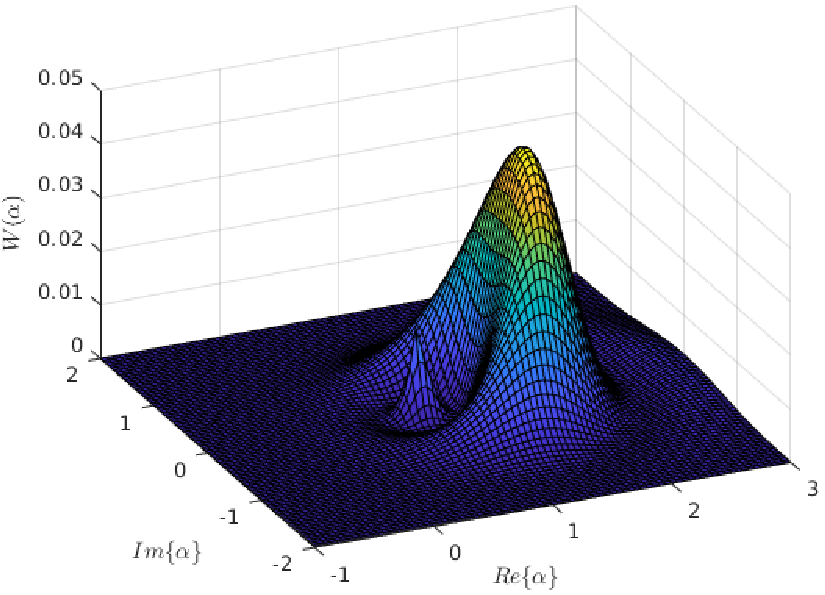
\includegraphics[width=\linewidth]{Pictures/WigPACS.pdf}
                    % This file was created by matlab2tikz.
%
%The latest updates can be retrieved from
%  http://www.mathworks.com/matlabcentral/fileexchange/22022-matlab2tikz-matlab2tikz
%where you can also make suggestions and rate matlab2tikz.
%
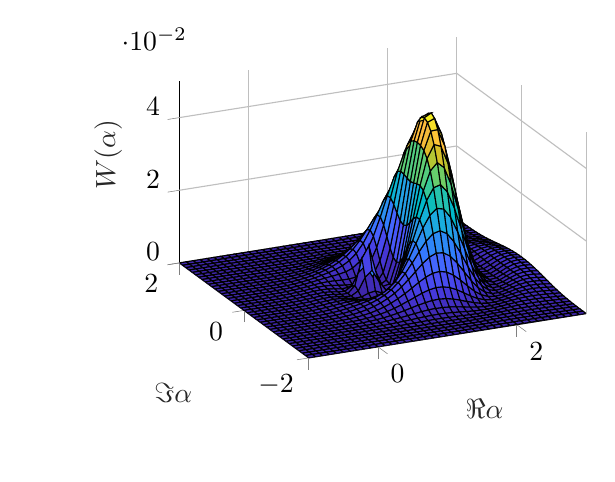
\begin{tikzpicture}

\begin{axis}[%
width=4.521in*0.45,
height=3.566in*0.45,
at={(0.758in,0.481in)},
scale only axis,
xmin=-1,
xmax=3,
tick align=outside,
xlabel style={font=\color{white!15!black}},
xlabel={$\Re{ \alpha }$},
ymin=-2,
ymax=2,
ylabel style={font=\color{white!15!black}},
ylabel={$\Im{ \alpha }$},
zmin=0,
zmax=0.05,
zlabel style={font=\color{white!15!black}},
zlabel={$W( \alpha )$},
view={-25}{30},
axis background/.style={fill=white},
axis x line*=bottom,
axis y line*=left,
axis z line*=left,
xmajorgrids,
ymajorgrids,
zmajorgrids
]

\addplot3[%
surf,
shader=flat corner, draw=black, z buffer=sort, colormap={mymap}{[1pt] rgb(0pt)=(0.2422,0.1504,0.6603); rgb(1pt)=(0.2444,0.1534,0.6728); rgb(2pt)=(0.2464,0.1569,0.6847); rgb(3pt)=(0.2484,0.1607,0.6961); rgb(4pt)=(0.2503,0.1648,0.7071); rgb(5pt)=(0.2522,0.1689,0.7179); rgb(6pt)=(0.254,0.1732,0.7286); rgb(7pt)=(0.2558,0.1773,0.7393); rgb(8pt)=(0.2576,0.1814,0.7501); rgb(9pt)=(0.2594,0.1854,0.761); rgb(11pt)=(0.2628,0.1932,0.7828); rgb(12pt)=(0.2645,0.1972,0.7937); rgb(13pt)=(0.2661,0.2011,0.8043); rgb(14pt)=(0.2676,0.2052,0.8148); rgb(15pt)=(0.2691,0.2094,0.8249); rgb(16pt)=(0.2704,0.2138,0.8346); rgb(17pt)=(0.2717,0.2184,0.8439); rgb(18pt)=(0.2729,0.2231,0.8528); rgb(19pt)=(0.274,0.228,0.8612); rgb(20pt)=(0.2749,0.233,0.8692); rgb(21pt)=(0.2758,0.2382,0.8767); rgb(22pt)=(0.2766,0.2435,0.884); rgb(23pt)=(0.2774,0.2489,0.8908); rgb(24pt)=(0.2781,0.2543,0.8973); rgb(25pt)=(0.2788,0.2598,0.9035); rgb(26pt)=(0.2794,0.2653,0.9094); rgb(27pt)=(0.2798,0.2708,0.915); rgb(28pt)=(0.2802,0.2764,0.9204); rgb(29pt)=(0.2806,0.2819,0.9255); rgb(30pt)=(0.2809,0.2875,0.9305); rgb(31pt)=(0.2811,0.293,0.9352); rgb(32pt)=(0.2813,0.2985,0.9397); rgb(33pt)=(0.2814,0.304,0.9441); rgb(34pt)=(0.2814,0.3095,0.9483); rgb(35pt)=(0.2813,0.315,0.9524); rgb(36pt)=(0.2811,0.3204,0.9563); rgb(37pt)=(0.2809,0.3259,0.96); rgb(38pt)=(0.2807,0.3313,0.9636); rgb(39pt)=(0.2803,0.3367,0.967); rgb(40pt)=(0.2798,0.3421,0.9702); rgb(41pt)=(0.2791,0.3475,0.9733); rgb(42pt)=(0.2784,0.3529,0.9763); rgb(43pt)=(0.2776,0.3583,0.9791); rgb(44pt)=(0.2766,0.3638,0.9817); rgb(45pt)=(0.2754,0.3693,0.984); rgb(46pt)=(0.2741,0.3748,0.9862); rgb(47pt)=(0.2726,0.3804,0.9881); rgb(48pt)=(0.271,0.386,0.9898); rgb(49pt)=(0.2691,0.3916,0.9912); rgb(50pt)=(0.267,0.3973,0.9924); rgb(51pt)=(0.2647,0.403,0.9935); rgb(52pt)=(0.2621,0.4088,0.9946); rgb(53pt)=(0.2591,0.4145,0.9955); rgb(54pt)=(0.2556,0.4203,0.9965); rgb(55pt)=(0.2517,0.4261,0.9974); rgb(56pt)=(0.2473,0.4319,0.9983); rgb(57pt)=(0.2424,0.4378,0.9991); rgb(58pt)=(0.2369,0.4437,0.9996); rgb(59pt)=(0.2311,0.4497,0.9995); rgb(60pt)=(0.225,0.4559,0.9985); rgb(61pt)=(0.2189,0.462,0.9968); rgb(62pt)=(0.2128,0.4682,0.9948); rgb(63pt)=(0.2066,0.4743,0.9926); rgb(64pt)=(0.2006,0.4803,0.9906); rgb(65pt)=(0.195,0.4861,0.9887); rgb(66pt)=(0.1903,0.4919,0.9867); rgb(67pt)=(0.1869,0.4975,0.9844); rgb(68pt)=(0.1847,0.503,0.9819); rgb(69pt)=(0.1831,0.5084,0.9793); rgb(70pt)=(0.1818,0.5138,0.9766); rgb(71pt)=(0.1806,0.5191,0.9738); rgb(72pt)=(0.1795,0.5244,0.9709); rgb(73pt)=(0.1785,0.5296,0.9677); rgb(74pt)=(0.1778,0.5349,0.9641); rgb(75pt)=(0.1773,0.5401,0.9602); rgb(76pt)=(0.1768,0.5452,0.956); rgb(77pt)=(0.1764,0.5504,0.9516); rgb(78pt)=(0.1755,0.5554,0.9473); rgb(79pt)=(0.174,0.5605,0.9432); rgb(80pt)=(0.1716,0.5655,0.9393); rgb(81pt)=(0.1686,0.5705,0.9357); rgb(82pt)=(0.1649,0.5755,0.9323); rgb(83pt)=(0.161,0.5805,0.9289); rgb(84pt)=(0.1573,0.5854,0.9254); rgb(85pt)=(0.154,0.5902,0.9218); rgb(86pt)=(0.1513,0.595,0.9182); rgb(87pt)=(0.1492,0.5997,0.9147); rgb(88pt)=(0.1475,0.6043,0.9113); rgb(89pt)=(0.1461,0.6089,0.908); rgb(90pt)=(0.1446,0.6135,0.905); rgb(91pt)=(0.1429,0.618,0.9022); rgb(92pt)=(0.1408,0.6226,0.8998); rgb(93pt)=(0.1383,0.6272,0.8975); rgb(94pt)=(0.1354,0.6317,0.8953); rgb(95pt)=(0.1321,0.6363,0.8932); rgb(96pt)=(0.1288,0.6408,0.891); rgb(97pt)=(0.1253,0.6453,0.8887); rgb(98pt)=(0.1219,0.6497,0.8862); rgb(99pt)=(0.1185,0.6541,0.8834); rgb(100pt)=(0.1152,0.6584,0.8804); rgb(101pt)=(0.1119,0.6627,0.877); rgb(102pt)=(0.1085,0.6669,0.8734); rgb(103pt)=(0.1048,0.671,0.8695); rgb(104pt)=(0.1009,0.675,0.8653); rgb(105pt)=(0.0964,0.6789,0.8609); rgb(106pt)=(0.0914,0.6828,0.8562); rgb(107pt)=(0.0855,0.6865,0.8513); rgb(108pt)=(0.0789,0.6902,0.8462); rgb(109pt)=(0.0713,0.6938,0.8409); rgb(110pt)=(0.0628,0.6972,0.8355); rgb(111pt)=(0.0535,0.7006,0.8299); rgb(112pt)=(0.0433,0.7039,0.8242); rgb(113pt)=(0.0328,0.7071,0.8183); rgb(114pt)=(0.0234,0.7103,0.8124); rgb(115pt)=(0.0155,0.7133,0.8064); rgb(116pt)=(0.0091,0.7163,0.8003); rgb(117pt)=(0.0046,0.7192,0.7941); rgb(118pt)=(0.0019,0.722,0.7878); rgb(119pt)=(0.0009,0.7248,0.7815); rgb(120pt)=(0.0018,0.7275,0.7752); rgb(121pt)=(0.0046,0.7301,0.7688); rgb(122pt)=(0.0094,0.7327,0.7623); rgb(123pt)=(0.0162,0.7352,0.7558); rgb(124pt)=(0.0253,0.7376,0.7492); rgb(125pt)=(0.0369,0.74,0.7426); rgb(126pt)=(0.0504,0.7423,0.7359); rgb(127pt)=(0.0638,0.7446,0.7292); rgb(128pt)=(0.077,0.7468,0.7224); rgb(129pt)=(0.0899,0.7489,0.7156); rgb(130pt)=(0.1023,0.751,0.7088); rgb(131pt)=(0.1141,0.7531,0.7019); rgb(132pt)=(0.1252,0.7552,0.695); rgb(133pt)=(0.1354,0.7572,0.6881); rgb(134pt)=(0.1448,0.7593,0.6812); rgb(135pt)=(0.1532,0.7614,0.6741); rgb(136pt)=(0.1609,0.7635,0.6671); rgb(137pt)=(0.1678,0.7656,0.6599); rgb(138pt)=(0.1741,0.7678,0.6527); rgb(139pt)=(0.1799,0.7699,0.6454); rgb(140pt)=(0.1853,0.7721,0.6379); rgb(141pt)=(0.1905,0.7743,0.6303); rgb(142pt)=(0.1954,0.7765,0.6225); rgb(143pt)=(0.2003,0.7787,0.6146); rgb(144pt)=(0.2061,0.7808,0.6065); rgb(145pt)=(0.2118,0.7828,0.5983); rgb(146pt)=(0.2178,0.7849,0.5899); rgb(147pt)=(0.2244,0.7869,0.5813); rgb(148pt)=(0.2318,0.7887,0.5725); rgb(149pt)=(0.2401,0.7905,0.5636); rgb(150pt)=(0.2491,0.7922,0.5546); rgb(151pt)=(0.2589,0.7937,0.5454); rgb(152pt)=(0.2695,0.7951,0.536); rgb(153pt)=(0.2809,0.7964,0.5266); rgb(154pt)=(0.2929,0.7975,0.517); rgb(155pt)=(0.3052,0.7985,0.5074); rgb(156pt)=(0.3176,0.7994,0.4975); rgb(157pt)=(0.3301,0.8002,0.4876); rgb(158pt)=(0.3424,0.8009,0.4774); rgb(159pt)=(0.3548,0.8016,0.4669); rgb(160pt)=(0.3671,0.8021,0.4563); rgb(161pt)=(0.3795,0.8026,0.4454); rgb(162pt)=(0.3921,0.8029,0.4344); rgb(163pt)=(0.405,0.8031,0.4233); rgb(164pt)=(0.4184,0.803,0.4122); rgb(165pt)=(0.4322,0.8028,0.4013); rgb(166pt)=(0.4463,0.8024,0.3904); rgb(167pt)=(0.4608,0.8018,0.3797); rgb(168pt)=(0.4753,0.8011,0.3691); rgb(169pt)=(0.4899,0.8002,0.3586); rgb(170pt)=(0.5044,0.7993,0.348); rgb(171pt)=(0.5187,0.7982,0.3374); rgb(172pt)=(0.5329,0.797,0.3267); rgb(173pt)=(0.547,0.7957,0.3159); rgb(175pt)=(0.5748,0.7929,0.2941); rgb(176pt)=(0.5886,0.7913,0.2833); rgb(177pt)=(0.6024,0.7896,0.2726); rgb(178pt)=(0.6161,0.7878,0.2622); rgb(179pt)=(0.6297,0.7859,0.2521); rgb(180pt)=(0.6433,0.7839,0.2423); rgb(181pt)=(0.6567,0.7818,0.2329); rgb(182pt)=(0.6701,0.7796,0.2239); rgb(183pt)=(0.6833,0.7773,0.2155); rgb(184pt)=(0.6963,0.775,0.2075); rgb(185pt)=(0.7091,0.7727,0.1998); rgb(186pt)=(0.7218,0.7703,0.1924); rgb(187pt)=(0.7344,0.7679,0.1852); rgb(188pt)=(0.7468,0.7654,0.1782); rgb(189pt)=(0.759,0.7629,0.1717); rgb(190pt)=(0.771,0.7604,0.1658); rgb(191pt)=(0.7829,0.7579,0.1608); rgb(192pt)=(0.7945,0.7554,0.157); rgb(193pt)=(0.806,0.7529,0.1546); rgb(194pt)=(0.8172,0.7505,0.1535); rgb(195pt)=(0.8281,0.7481,0.1536); rgb(196pt)=(0.8389,0.7457,0.1546); rgb(197pt)=(0.8495,0.7435,0.1564); rgb(198pt)=(0.86,0.7413,0.1587); rgb(199pt)=(0.8703,0.7392,0.1615); rgb(200pt)=(0.8804,0.7372,0.165); rgb(201pt)=(0.8903,0.7353,0.1695); rgb(202pt)=(0.9,0.7336,0.1749); rgb(203pt)=(0.9093,0.7321,0.1815); rgb(204pt)=(0.9184,0.7308,0.189); rgb(205pt)=(0.9272,0.7298,0.1973); rgb(206pt)=(0.9357,0.729,0.2061); rgb(207pt)=(0.944,0.7285,0.2151); rgb(208pt)=(0.9523,0.7284,0.2237); rgb(209pt)=(0.9606,0.7285,0.2312); rgb(210pt)=(0.9689,0.7292,0.2373); rgb(211pt)=(0.977,0.7304,0.2418); rgb(212pt)=(0.9842,0.733,0.2446); rgb(213pt)=(0.99,0.7365,0.2429); rgb(214pt)=(0.9946,0.7407,0.2394); rgb(215pt)=(0.9966,0.7458,0.2351); rgb(216pt)=(0.9971,0.7513,0.2309); rgb(217pt)=(0.9972,0.7569,0.2267); rgb(218pt)=(0.9971,0.7626,0.2224); rgb(219pt)=(0.9969,0.7683,0.2181); rgb(220pt)=(0.9966,0.774,0.2138); rgb(221pt)=(0.9962,0.7798,0.2095); rgb(222pt)=(0.9957,0.7856,0.2053); rgb(223pt)=(0.9949,0.7915,0.2012); rgb(224pt)=(0.9938,0.7974,0.1974); rgb(225pt)=(0.9923,0.8034,0.1939); rgb(226pt)=(0.9906,0.8095,0.1906); rgb(227pt)=(0.9885,0.8156,0.1875); rgb(228pt)=(0.9861,0.8218,0.1846); rgb(229pt)=(0.9835,0.828,0.1817); rgb(230pt)=(0.9807,0.8342,0.1787); rgb(231pt)=(0.9778,0.8404,0.1757); rgb(232pt)=(0.9748,0.8467,0.1726); rgb(233pt)=(0.972,0.8529,0.1695); rgb(234pt)=(0.9694,0.8591,0.1665); rgb(235pt)=(0.9671,0.8654,0.1636); rgb(236pt)=(0.9651,0.8716,0.1608); rgb(237pt)=(0.9634,0.8778,0.1582); rgb(238pt)=(0.9619,0.884,0.1557); rgb(239pt)=(0.9608,0.8902,0.1532); rgb(240pt)=(0.9601,0.8963,0.1507); rgb(241pt)=(0.9596,0.9023,0.148); rgb(242pt)=(0.9595,0.9084,0.145); rgb(243pt)=(0.9597,0.9143,0.1418); rgb(244pt)=(0.9601,0.9203,0.1382); rgb(245pt)=(0.9608,0.9262,0.1344); rgb(246pt)=(0.9618,0.932,0.1304); rgb(247pt)=(0.9629,0.9379,0.1261); rgb(248pt)=(0.9642,0.9437,0.1216); rgb(249pt)=(0.9657,0.9494,0.1168); rgb(250pt)=(0.9674,0.9552,0.1116); rgb(251pt)=(0.9692,0.9609,0.1061); rgb(252pt)=(0.9711,0.9667,0.1001); rgb(253pt)=(0.973,0.9724,0.0938); rgb(254pt)=(0.9749,0.9782,0.0872); rgb(255pt)=(0.9769,0.9839,0.0805)}, mesh/rows=41]
table[row sep=crcr, point meta=\thisrow{c}] {%
%
x	y	z	c\\
-1	-2	1.27459273151555e-09	1.27459273151555e-09\\
-1	-1.9	2.21577590523692e-09	2.21577590523692e-09\\
-1	-1.8	3.66202150570177e-09	3.66202150570177e-09\\
-1	-1.7	5.74862875186445e-09	5.74862875186445e-09\\
-1	-1.6	8.56274817555437e-09	8.56274817555437e-09\\
-1	-1.5	1.20883097013998e-08	1.20883097013998e-08\\
-1	-1.4	1.61528730097932e-08	1.61528730097932e-08\\
-1	-1.3	2.03991713356433e-08	2.03991713356433e-08\\
-1	-1.2	2.43055994566938e-08	2.43055994566938e-08\\
-1	-1.1	2.72695509214837e-08	2.72695509214837e-08\\
-1	-1	2.87450459936329e-08	2.87450459936329e-08\\
-1	-0.9	2.83986169525942e-08	2.83986169525942e-08\\
-1	-0.8	2.62282409498986e-08	2.62282409498986e-08\\
-1	-0.7	2.25925990318261e-08	2.25925990318261e-08\\
-1	-0.6	1.81269222563538e-08	1.81269222563538e-08\\
-1	-0.5	1.35678276947833e-08	1.35678276947833e-08\\
-1	-0.4	9.55162376652154e-09	9.55162376652154e-09\\
-1	-0.3	6.46597831011493e-09	6.46597831011493e-09\\
-1	-0.2	4.41280263196691e-09	4.41280263196691e-09\\
-1	-0.0999999999999999	3.28925766818567e-09	3.28925766818567e-09\\
-1	0	2.93843510054073e-09	2.93843510054073e-09\\
-1	0.0999999999999999	3.28925766818567e-09	3.28925766818567e-09\\
-1	0.2	4.41280263196691e-09	4.41280263196691e-09\\
-1	0.3	6.46597831011493e-09	6.46597831011493e-09\\
-1	0.4	9.55162376652154e-09	9.55162376652154e-09\\
-1	0.5	1.35678276947833e-08	1.35678276947833e-08\\
-1	0.6	1.81269222563538e-08	1.81269222563538e-08\\
-1	0.7	2.25925990318261e-08	2.25925990318261e-08\\
-1	0.8	2.62282409498986e-08	2.62282409498986e-08\\
-1	0.9	2.83986169525942e-08	2.83986169525942e-08\\
-1	1	2.87450459936329e-08	2.87450459936329e-08\\
-1	1.1	2.72695509214837e-08	2.72695509214837e-08\\
-1	1.2	2.43055994566938e-08	2.43055994566938e-08\\
-1	1.3	2.03991713356433e-08	2.03991713356433e-08\\
-1	1.4	1.61528730097932e-08	1.61528730097932e-08\\
-1	1.5	1.20883097013998e-08	1.20883097013998e-08\\
-1	1.6	8.56274817555437e-09	8.56274817555437e-09\\
-1	1.7	5.74862875186445e-09	5.74862875186445e-09\\
-1	1.8	3.66202150570177e-09	3.66202150570177e-09\\
-1	1.9	2.21577590523692e-09	2.21577590523692e-09\\
-1	2	1.27459273151555e-09	1.27459273151555e-09\\
-0.9	-2	2.78975853923214e-09	2.78975853923214e-09\\
-0.9	-1.9	4.75022763558817e-09	4.75022763558817e-09\\
-0.9	-1.8	7.6633782680446e-09	7.6633782680446e-09\\
-0.9	-1.7	1.16934217040638e-08	1.16934217040638e-08\\
-0.9	-1.6	1.68411595165278e-08	1.68411595165278e-08\\
-0.9	-1.5	2.28340749716608e-08	2.28340749716608e-08\\
-0.9	-1.4	2.90496177078623e-08	2.90496177078623e-08\\
-0.9	-1.3	3.45276296721333e-08	3.45276296721333e-08\\
-0.9	-1.2	3.81180208058163e-08	3.81180208058163e-08\\
-0.9	-1.1	3.87683371308878e-08	3.87683371308878e-08\\
-0.9	-1	3.58894426323992e-08	3.58894426323992e-08\\
-0.9	-0.9	2.96726598138189e-08	2.96726598138189e-08\\
-0.9	-0.8	2.12067773444405e-08	2.12067773444405e-08\\
-0.9	-0.7	1.22881925931044e-08	1.22881925931044e-08\\
-0.9	-0.6	4.93048894606257e-09	4.93048894606257e-09\\
-0.9	-0.5	7.18557121378036e-10	7.18557121378036e-10\\
-0.9	-0.4	2.49208236789367e-10	2.49208236789367e-10\\
-0.9	-0.3	2.89747280631114e-09	2.89747280631114e-09\\
-0.9	-0.2	7.03305492155211e-09	7.03305492155211e-09\\
-0.9	-0.0999999999999999	1.06292781645676e-08	1.06292781645676e-08\\
-0.9	0	1.20383804913276e-08	1.20383804913276e-08\\
-0.9	0.0999999999999999	1.06292781645676e-08	1.06292781645676e-08\\
-0.9	0.2	7.03305492155211e-09	7.03305492155211e-09\\
-0.9	0.3	2.89747280631114e-09	2.89747280631114e-09\\
-0.9	0.4	2.49208236789367e-10	2.49208236789367e-10\\
-0.9	0.5	7.18557121378036e-10	7.18557121378036e-10\\
-0.9	0.6	4.93048894606257e-09	4.93048894606257e-09\\
-0.9	0.7	1.22881925931044e-08	1.22881925931044e-08\\
-0.9	0.8	2.12067773444405e-08	2.12067773444405e-08\\
-0.9	0.9	2.96726598138189e-08	2.96726598138189e-08\\
-0.9	1	3.58894426323992e-08	3.58894426323992e-08\\
-0.9	1.1	3.87683371308878e-08	3.87683371308878e-08\\
-0.9	1.2	3.81180208058163e-08	3.81180208058163e-08\\
-0.9	1.3	3.45276296721333e-08	3.45276296721333e-08\\
-0.9	1.4	2.90496177078623e-08	2.90496177078623e-08\\
-0.9	1.5	2.28340749716608e-08	2.28340749716608e-08\\
-0.9	1.6	1.68411595165278e-08	1.68411595165278e-08\\
-0.9	1.7	1.16934217040638e-08	1.16934217040638e-08\\
-0.9	1.8	7.6633782680446e-09	7.6633782680446e-09\\
-0.9	1.9	4.75022763558817e-09	4.75022763558817e-09\\
-0.9	2	2.78975853923214e-09	2.78975853923214e-09\\
-0.8	-2	5.83932232575003e-09	5.83932232575003e-09\\
-0.8	-1.9	9.71391456361138e-09	9.71391456361138e-09\\
-0.8	-1.8	1.5243022689019e-08	1.5243022689019e-08\\
-0.8	-1.7	2.24959409176574e-08	2.24959409176574e-08\\
-0.8	-1.6	3.11039783489143e-08	3.11039783489143e-08\\
-0.8	-1.5	4.00824253937516e-08	4.00824253937516e-08\\
-0.8	-1.4	4.77943788222459e-08	4.77943788222459e-08\\
-0.8	-1.3	5.21782177707213e-08	5.21782177707213e-08\\
-0.8	-1.2	5.13029489989409e-08	5.13029489989409e-08\\
-0.8	-1.1	4.41819183504569e-08	4.41819183504569e-08\\
-0.8	-1	3.16011392967092e-08	3.16011392967092e-08\\
-0.8	-0.9	1.65873250009922e-08	1.65873250009922e-08\\
-0.8	-0.8	4.15187076924586e-09	4.15187076924586e-09\\
-0.8	-0.7	1.54954411436771e-10	1.54954411436771e-10\\
-0.8	-0.6	9.49363113002291e-09	9.49363113002291e-09\\
-0.8	-0.5	3.41800436039146e-08	3.41800436039146e-08\\
-0.8	-0.4	7.20518146789612e-08	7.20518146789612e-08\\
-0.8	-0.3	1.16723378457605e-07	1.16723378457605e-07\\
-0.8	-0.2	1.58967550455102e-07	1.58967550455102e-07\\
-0.8	-0.0999999999999999	1.89178758803821e-07	1.89178758803821e-07\\
-0.8	0	2.00140819464434e-07	2.00140819464434e-07\\
-0.8	0.0999999999999999	1.89178758803821e-07	1.89178758803821e-07\\
-0.8	0.2	1.58967550455102e-07	1.58967550455102e-07\\
-0.8	0.3	1.16723378457605e-07	1.16723378457605e-07\\
-0.8	0.4	7.20518146789612e-08	7.20518146789612e-08\\
-0.8	0.5	3.41800436039146e-08	3.41800436039146e-08\\
-0.8	0.6	9.49363113002291e-09	9.49363113002291e-09\\
-0.8	0.7	1.54954411436771e-10	1.54954411436771e-10\\
-0.8	0.8	4.15187076924586e-09	4.15187076924586e-09\\
-0.8	0.9	1.65873250009922e-08	1.65873250009922e-08\\
-0.8	1	3.16011392967092e-08	3.16011392967092e-08\\
-0.8	1.1	4.41819183504569e-08	4.41819183504569e-08\\
-0.8	1.2	5.13029489989409e-08	5.13029489989409e-08\\
-0.8	1.3	5.21782177707213e-08	5.21782177707213e-08\\
-0.8	1.4	4.77943788222459e-08	4.77943788222459e-08\\
-0.8	1.5	4.00824253937516e-08	4.00824253937516e-08\\
-0.8	1.6	3.11039783489143e-08	3.11039783489143e-08\\
-0.8	1.7	2.24959409176574e-08	2.24959409176574e-08\\
-0.8	1.8	1.5243022689019e-08	1.5243022689019e-08\\
-0.8	1.9	9.71391456361138e-09	9.71391456361138e-09\\
-0.8	2	5.83932232575003e-09	5.83932232575003e-09\\
-0.7	-2	1.16921796882645e-08	1.16921796882645e-08\\
-0.7	-1.9	1.89473346137208e-08	1.89473346137208e-08\\
-0.7	-1.8	2.87982346825092e-08	2.87982346825092e-08\\
-0.7	-1.7	4.08513368984665e-08	4.08513368984665e-08\\
-0.7	-1.6	5.37151995059036e-08	5.37151995059036e-08\\
-0.7	-1.5	6.48219145110286e-08	6.48219145110286e-08\\
-0.7	-1.4	7.0701404556289e-08	7.0701404556289e-08\\
-0.7	-1.3	6.79380220885067e-08	6.79380220885067e-08\\
-0.7	-1.2	5.48269109088252e-08	5.48269109088252e-08\\
-0.7	-1.1	3.33714712097303e-08	3.33714712097303e-08\\
-0.7	-1	1.08537430825073e-08	1.08537430825073e-08\\
-0.7	-0.9	1.25770059883178e-12	1.25770059883178e-12\\
-0.7	-0.8	1.69971447738974e-08	1.69971447738974e-08\\
-0.7	-0.7	7.7298151771822e-08	7.7298151771822e-08\\
-0.7	-0.6	1.90220147116693e-07	1.90220147116693e-07\\
-0.7	-0.5	3.54069360682003e-07	3.54069360682003e-07\\
-0.7	-0.4	5.53774599036888e-07	5.53774599036888e-07\\
-0.7	-0.3	7.62316142140354e-07	7.62316142140354e-07\\
-0.7	-0.2	9.4597415858807e-07	9.4597415858807e-07\\
-0.7	-0.0999999999999999	1.07206697517096e-06	1.07206697517096e-06\\
-0.7	0	1.11696727051389e-06	1.11696727051389e-06\\
-0.7	0.0999999999999999	1.07206697517096e-06	1.07206697517096e-06\\
-0.7	0.2	9.4597415858807e-07	9.4597415858807e-07\\
-0.7	0.3	7.62316142140354e-07	7.62316142140354e-07\\
-0.7	0.4	5.53774599036888e-07	5.53774599036888e-07\\
-0.7	0.5	3.54069360682003e-07	3.54069360682003e-07\\
-0.7	0.6	1.90220147116693e-07	1.90220147116693e-07\\
-0.7	0.7	7.7298151771822e-08	7.7298151771822e-08\\
-0.7	0.8	1.69971447738974e-08	1.69971447738974e-08\\
-0.7	0.9	1.25770059883178e-12	1.25770059883178e-12\\
-0.7	1	1.08537430825073e-08	1.08537430825073e-08\\
-0.7	1.1	3.33714712097303e-08	3.33714712097303e-08\\
-0.7	1.2	5.48269109088252e-08	5.48269109088252e-08\\
-0.7	1.3	6.79380220885067e-08	6.79380220885067e-08\\
-0.7	1.4	7.0701404556289e-08	7.0701404556289e-08\\
-0.7	1.5	6.48219145110286e-08	6.48219145110286e-08\\
-0.7	1.6	5.37151995059036e-08	5.37151995059036e-08\\
-0.7	1.7	4.08513368984665e-08	4.08513368984665e-08\\
-0.7	1.8	2.87982346825092e-08	2.87982346825092e-08\\
-0.7	1.9	1.89473346137208e-08	1.89473346137208e-08\\
-0.7	2	1.16921796882645e-08	1.16921796882645e-08\\
-0.6	-2	2.24064960207448e-08	2.24064960207448e-08\\
-0.6	-1.9	3.52544611886853e-08	3.52544611886853e-08\\
-0.6	-1.8	5.16403760978818e-08	5.16403760978818e-08\\
-0.6	-1.7	6.98579315123247e-08	6.98579315123247e-08\\
-0.6	-1.6	8.62404048302549e-08	8.62404048302549e-08\\
-0.6	-1.5	9.53307117451868e-08	9.53307117451868e-08\\
-0.6	-1.4	9.12855129761912e-08	9.12855129761912e-08\\
-0.6	-1.3	7.086008414402e-08	7.086008414402e-08\\
-0.6	-1.2	3.76790021196364e-08	3.76790021196364e-08\\
-0.6	-1.1	6.54664087412911e-09	6.54664087412911e-09\\
-0.6	-1	5.6939144924839e-09	5.6939144924839e-09\\
-0.6	-0.9	7.46926734800526e-08	7.46926734800526e-08\\
-0.6	-0.8	2.56770340963872e-07	2.56770340963872e-07\\
-0.6	-0.7	5.86369888803929e-07	5.86369888803929e-07\\
-0.6	-0.6	1.07524601039761e-06	1.07524601039761e-06\\
-0.6	-0.5	1.70193138968186e-06	1.70193138968186e-06\\
-0.6	-0.4	2.40903878852551e-06	2.40903878852551e-06\\
-0.6	-0.3	3.11049659797649e-06	3.11049659797649e-06\\
-0.6	-0.2	3.70744329333853e-06	3.70744329333853e-06\\
-0.6	-0.0999999999999999	4.10864328918489e-06	4.10864328918489e-06\\
-0.6	0	4.25004642252465e-06	4.25004642252465e-06\\
-0.6	0.0999999999999999	4.10864328918489e-06	4.10864328918489e-06\\
-0.6	0.2	3.70744329333853e-06	3.70744329333853e-06\\
-0.6	0.3	3.11049659797649e-06	3.11049659797649e-06\\
-0.6	0.4	2.40903878852551e-06	2.40903878852551e-06\\
-0.6	0.5	1.70193138968186e-06	1.70193138968186e-06\\
-0.6	0.6	1.07524601039761e-06	1.07524601039761e-06\\
-0.6	0.7	5.86369888803929e-07	5.86369888803929e-07\\
-0.6	0.8	2.56770340963872e-07	2.56770340963872e-07\\
-0.6	0.9	7.46926734800526e-08	7.46926734800526e-08\\
-0.6	1	5.6939144924839e-09	5.6939144924839e-09\\
-0.6	1.1	6.54664087412911e-09	6.54664087412911e-09\\
-0.6	1.2	3.76790021196364e-08	3.76790021196364e-08\\
-0.6	1.3	7.086008414402e-08	7.086008414402e-08\\
-0.6	1.4	9.12855129761912e-08	9.12855129761912e-08\\
-0.6	1.5	9.53307117451868e-08	9.53307117451868e-08\\
-0.6	1.6	8.62404048302549e-08	8.62404048302549e-08\\
-0.6	1.7	6.98579315123247e-08	6.98579315123247e-08\\
-0.6	1.8	5.16403760978818e-08	5.16403760978818e-08\\
-0.6	1.9	3.52544611886853e-08	3.52544611886853e-08\\
-0.6	2	2.24064960207448e-08	2.24064960207448e-08\\
-0.5	-2	4.11243338472045e-08	4.11243338472045e-08\\
-0.5	-1.9	6.25907560760325e-08	6.25907560760325e-08\\
-0.5	-1.8	8.78275374927728e-08	8.78275374927728e-08\\
-0.5	-1.7	1.12162988413547e-07	1.12162988413547e-07\\
-0.5	-1.6	1.27679371905627e-07	1.27679371905627e-07\\
-0.5	-1.5	1.2483752818067e-07	1.2483752818067e-07\\
-0.5	-1.4	9.70999235770076e-08	9.70999235770076e-08\\
-0.5	-1.3	4.88498632433124e-08	4.88498632433124e-08\\
-0.5	-1.2	5.19118878740651e-09	5.19118878740651e-09\\
-0.5	-1.1	2.00223758597106e-08	2.00223758597106e-08\\
-0.5	-1	1.77218867548876e-07	1.77218867548876e-07\\
-0.5	-0.9	5.80233841721344e-07	5.80233841721344e-07\\
-0.5	-0.8	1.32877385644209e-06	1.32877385644209e-06\\
-0.5	-0.7	2.48675628826193e-06	2.48675628826193e-06\\
-0.5	-0.6	4.05112538288415e-06	4.05112538288415e-06\\
-0.5	-0.5	5.93320731793504e-06	5.93320731793504e-06\\
-0.5	-0.4	7.961260330361e-06	7.961260330361e-06\\
-0.5	-0.3	9.90564149184984e-06	9.90564149184984e-06\\
-0.5	-0.2	1.15200659209269e-05	1.15200659209269e-05\\
-0.5	-0.0999999999999999	1.25876951892808e-05	1.25876951892808e-05\\
-0.5	0	1.29609654149084e-05	1.29609654149084e-05\\
-0.5	0.0999999999999999	1.25876951892808e-05	1.25876951892808e-05\\
-0.5	0.2	1.15200659209269e-05	1.15200659209269e-05\\
-0.5	0.3	9.90564149184984e-06	9.90564149184984e-06\\
-0.5	0.4	7.961260330361e-06	7.961260330361e-06\\
-0.5	0.5	5.93320731793504e-06	5.93320731793504e-06\\
-0.5	0.6	4.05112538288415e-06	4.05112538288415e-06\\
-0.5	0.7	2.48675628826193e-06	2.48675628826193e-06\\
-0.5	0.8	1.32877385644209e-06	1.32877385644209e-06\\
-0.5	0.9	5.80233841721344e-07	5.80233841721344e-07\\
-0.5	1	1.77218867548876e-07	1.77218867548876e-07\\
-0.5	1.1	2.00223758597106e-08	2.00223758597106e-08\\
-0.5	1.2	5.19118878740651e-09	5.19118878740651e-09\\
-0.5	1.3	4.88498632433124e-08	4.88498632433124e-08\\
-0.5	1.4	9.70999235770076e-08	9.70999235770076e-08\\
-0.5	1.5	1.2483752818067e-07	1.2483752818067e-07\\
-0.5	1.6	1.27679371905627e-07	1.27679371905627e-07\\
-0.5	1.7	1.12162988413547e-07	1.12162988413547e-07\\
-0.5	1.8	8.78275374927728e-08	8.78275374927728e-08\\
-0.5	1.9	6.25907560760325e-08	6.25907560760325e-08\\
-0.5	2	4.11243338472045e-08	4.11243338472045e-08\\
-0.4	-2	7.23586052331808e-08	7.23586052331808e-08\\
-0.4	-1.9	1.06088513115266e-07	1.06088513115266e-07\\
-0.4	-1.8	1.41580806224711e-07	1.41580806224711e-07\\
-0.4	-1.7	1.68453438674514e-07	1.68453438674514e-07\\
-0.4	-1.6	1.72216275026527e-07	1.72216275026527e-07\\
-0.4	-1.5	1.40193804750053e-07	1.40193804750053e-07\\
-0.4	-1.4	7.40634670188731e-08	7.40634670188731e-08\\
-0.4	-1.3	8.53253854271282e-09	8.53253854271282e-09\\
-0.4	-1.2	3.15199653730075e-08	3.15199653730075e-08\\
-0.4	-1.1	2.9659257430806e-07	2.9659257430806e-07\\
-0.4	-1	1.01611521036167e-06	1.01611521036167e-06\\
-0.4	-0.9	2.42666457943326e-06	2.42666457943326e-06\\
-0.4	-0.8	4.72784997678875e-06	4.72784997678875e-06\\
-0.4	-0.7	8.00899215528903e-06	8.00899215528903e-06\\
-0.4	-0.6	1.2188549348277e-05	1.2188549348277e-05\\
-0.4	-0.5	1.69916112183328e-05	1.69916112183328e-05\\
-0.4	-0.4	2.19785618874719e-05	2.19785618874719e-05\\
-0.4	-0.3	2.66181960878687e-05	2.66181960878687e-05\\
-0.4	-0.2	3.0381878806007e-05	3.0381878806007e-05\\
-0.4	-0.0999999999999999	3.28311446248063e-05	3.28311446248063e-05\\
-0.4	0	3.36804344381894e-05	3.36804344381894e-05\\
-0.4	0.0999999999999999	3.28311446248063e-05	3.28311446248063e-05\\
-0.4	0.2	3.0381878806007e-05	3.0381878806007e-05\\
-0.4	0.3	2.66181960878687e-05	2.66181960878687e-05\\
-0.4	0.4	2.19785618874719e-05	2.19785618874719e-05\\
-0.4	0.5	1.69916112183328e-05	1.69916112183328e-05\\
-0.4	0.6	1.2188549348277e-05	1.2188549348277e-05\\
-0.4	0.7	8.00899215528903e-06	8.00899215528903e-06\\
-0.4	0.8	4.72784997678875e-06	4.72784997678875e-06\\
-0.4	0.9	2.42666457943326e-06	2.42666457943326e-06\\
-0.4	1	1.01611521036167e-06	1.01611521036167e-06\\
-0.4	1.1	2.9659257430806e-07	2.9659257430806e-07\\
-0.4	1.2	3.15199653730075e-08	3.15199653730075e-08\\
-0.4	1.3	8.53253854271282e-09	8.53253854271282e-09\\
-0.4	1.4	7.40634670188731e-08	7.40634670188731e-08\\
-0.4	1.5	1.40193804750053e-07	1.40193804750053e-07\\
-0.4	1.6	1.72216275026527e-07	1.72216275026527e-07\\
-0.4	1.7	1.68453438674514e-07	1.68453438674514e-07\\
-0.4	1.8	1.41580806224711e-07	1.41580806224711e-07\\
-0.4	1.9	1.06088513115266e-07	1.06088513115266e-07\\
-0.4	2	7.23586052331808e-08	7.23586052331808e-08\\
-0.3	-2	1.22213189314101e-07	1.22213189314101e-07\\
-0.3	-1.9	1.71822785686703e-07	1.71822785686703e-07\\
-0.3	-1.8	2.16216096905593e-07	2.16216096905593e-07\\
-0.3	-1.7	2.35499973858008e-07	2.35499973858008e-07\\
-0.3	-1.6	2.07600384153127e-07	2.07600384153127e-07\\
-0.3	-1.5	1.24860632175885e-07	1.24860632175885e-07\\
-0.3	-1.4	2.39957603080685e-08	2.39957603080685e-08\\
-0.3	-1.3	2.59907826798851e-08	2.59907826798851e-08\\
-0.3	-1.2	3.7322893587386e-07	3.7322893587386e-07\\
-0.3	-1.1	1.4422372027909e-06	1.4422372027909e-06\\
-0.3	-1	3.70846193697604e-06	3.70846193697604e-06\\
-0.3	-0.9	7.65058710962608e-06	7.65058710962608e-06\\
-0.3	-0.8	1.36066652560263e-05	1.36066652560263e-05\\
-0.3	-0.7	2.16238059142237e-05	2.16238059142237e-05\\
-0.3	-0.6	3.1360588940092e-05	3.1360588940092e-05\\
-0.3	-0.5	4.20913381880503e-05	4.20913381880503e-05\\
-0.3	-0.4	5.28223112571309e-05	5.28223112571309e-05\\
-0.3	-0.3	6.2480017821574e-05	6.2480017821574e-05\\
-0.3	-0.2	7.0101044481137e-05	7.0101044481137e-05\\
-0.3	-0.0999999999999999	7.49617602596243e-05	7.49617602596243e-05\\
-0.3	0	7.66293284682343e-05	7.66293284682343e-05\\
-0.3	0.0999999999999999	7.49617602596243e-05	7.49617602596243e-05\\
-0.3	0.2	7.0101044481137e-05	7.0101044481137e-05\\
-0.3	0.3	6.2480017821574e-05	6.2480017821574e-05\\
-0.3	0.4	5.28223112571309e-05	5.28223112571309e-05\\
-0.3	0.5	4.20913381880503e-05	4.20913381880503e-05\\
-0.3	0.6	3.1360588940092e-05	3.1360588940092e-05\\
-0.3	0.7	2.16238059142237e-05	2.16238059142237e-05\\
-0.3	0.8	1.36066652560263e-05	1.36066652560263e-05\\
-0.3	0.9	7.65058710962608e-06	7.65058710962608e-06\\
-0.3	1	3.70846193697604e-06	3.70846193697604e-06\\
-0.3	1.1	1.4422372027909e-06	1.4422372027909e-06\\
-0.3	1.2	3.7322893587386e-07	3.7322893587386e-07\\
-0.3	1.3	2.59907826798851e-08	2.59907826798851e-08\\
-0.3	1.4	2.39957603080685e-08	2.39957603080685e-08\\
-0.3	1.5	1.24860632175885e-07	1.24860632175885e-07\\
-0.3	1.6	2.07600384153127e-07	2.07600384153127e-07\\
-0.3	1.7	2.35499973858008e-07	2.35499973858008e-07\\
-0.3	1.8	2.16216096905593e-07	2.16216096905593e-07\\
-0.3	1.9	1.71822785686703e-07	1.71822785686703e-07\\
-0.3	2	1.22213189314101e-07	1.22213189314101e-07\\
-0.2	-2	1.9849033486585e-07	1.9849033486585e-07\\
-0.2	-1.9	2.66294621754515e-07	2.66294621754515e-07\\
-0.2	-1.8	3.12742359067918e-07	3.12742359067918e-07\\
-0.2	-1.7	3.04477091054448e-07	3.04477091054448e-07\\
-0.2	-1.6	2.16296419325015e-07	2.16296419325015e-07\\
-0.2	-1.5	7.12756193858e-08	7.12756193858e-08\\
-0.2	-1.4	5.60431247372839e-09	5.60431247372839e-09\\
-0.2	-1.3	3.46426281953108e-07	3.46426281953108e-07\\
-0.2	-1.2	1.67159439449808e-06	1.67159439449808e-06\\
-0.2	-1.1	4.80467084529409e-06	4.80467084529409e-06\\
-0.2	-1	1.07010326973304e-05	1.07010326973304e-05\\
-0.2	-0.9	2.02130867700084e-05	2.02130867700084e-05\\
-0.2	-0.8	3.37814340108109e-05	3.37814340108109e-05\\
-0.2	-0.7	5.11595906472195e-05	5.11595906472195e-05\\
-0.2	-0.6	7.13026620869591e-05	7.13026620869591e-05\\
-0.2	-0.5	9.25039465579261e-05	9.25039465579261e-05\\
-0.2	-0.4	0.000112754470056662	0.000112754470056662\\
-0.2	-0.3	0.000130183956805355	0.000130183956805355\\
-0.2	-0.2	0.000143394159599602	0.000143394159599602\\
-0.2	-0.0999999999999999	0.000151559479095146	0.000151559479095146\\
-0.2	0	0.000154312517674551	0.000154312517674551\\
-0.2	0.0999999999999999	0.000151559479095146	0.000151559479095146\\
-0.2	0.2	0.000143394159599602	0.000143394159599602\\
-0.2	0.3	0.000130183956805355	0.000130183956805355\\
-0.2	0.4	0.000112754470056662	0.000112754470056662\\
-0.2	0.5	9.25039465579261e-05	9.25039465579261e-05\\
-0.2	0.6	7.13026620869591e-05	7.13026620869591e-05\\
-0.2	0.7	5.11595906472195e-05	5.11595906472195e-05\\
-0.2	0.8	3.37814340108109e-05	3.37814340108109e-05\\
-0.2	0.9	2.02130867700084e-05	2.02130867700084e-05\\
-0.2	1	1.07010326973304e-05	1.07010326973304e-05\\
-0.2	1.1	4.80467084529409e-06	4.80467084529409e-06\\
-0.2	1.2	1.67159439449808e-06	1.67159439449808e-06\\
-0.2	1.3	3.46426281953108e-07	3.46426281953108e-07\\
-0.2	1.4	5.60431247372839e-09	5.60431247372839e-09\\
-0.2	1.5	7.12756193858e-08	7.12756193858e-08\\
-0.2	1.6	2.16296419325015e-07	2.16296419325015e-07\\
-0.2	1.7	3.04477091054448e-07	3.04477091054448e-07\\
-0.2	1.8	3.12742359067918e-07	3.12742359067918e-07\\
-0.2	1.9	2.66294621754515e-07	2.66294621754515e-07\\
-0.2	2	1.9849033486585e-07	1.9849033486585e-07\\
-0.1	-2	3.10696886143478e-07	3.10696886143478e-07\\
-0.1	-1.9	3.95761011087356e-07	3.95761011087356e-07\\
-0.1	-1.8	4.28590235819867e-07	4.28590235819867e-07\\
-0.1	-1.7	3.60797052313021e-07	3.60797052313021e-07\\
-0.1	-1.6	1.8216673390269e-07	1.8216673390269e-07\\
-0.1	-1.5	7.92078188851616e-09	7.92078188851616e-09\\
-0.1	-1.4	2.07753006388355e-07	2.07753006388355e-07\\
-0.1	-1.3	1.54486588824065e-06	1.54486588824065e-06\\
-0.1	-1.2	5.25541211131346e-06	5.25541211131346e-06\\
-0.1	-1.1	1.29743399440226e-05	1.29743399440226e-05\\
-0.1	-1	2.64323151491427e-05	2.64323151491427e-05\\
-0.1	-0.9	4.69301230267347e-05	4.69301230267347e-05\\
-0.1	-0.8	7.47273636340481e-05	7.47273636340481e-05\\
-0.1	-0.7	0.000108599510795147	0.000108599510795147\\
-0.1	-0.6	0.000145831970272297	0.000145831970272297\\
-0.1	-0.5	0.000182771728245654	0.000182771728245654\\
-0.1	-0.4	0.000215781969783657	0.000215781969783657\\
-0.1	-0.3	0.000242190422435495	0.000242190422435495\\
-0.1	-0.2	0.000260772481421279	0.000260772481421279\\
-0.1	-0.0999999999999999	0.000271544541211384	0.000271544541211384\\
-0.1	0	0.00027504015035135	0.00027504015035135\\
-0.1	0.0999999999999999	0.000271544541211384	0.000271544541211384\\
-0.1	0.2	0.000260772481421279	0.000260772481421279\\
-0.1	0.3	0.000242190422435495	0.000242190422435495\\
-0.1	0.4	0.000215781969783657	0.000215781969783657\\
-0.1	0.5	0.000182771728245654	0.000182771728245654\\
-0.1	0.6	0.000145831970272297	0.000145831970272297\\
-0.1	0.7	0.000108599510795147	0.000108599510795147\\
-0.1	0.8	7.47273636340481e-05	7.47273636340481e-05\\
-0.1	0.9	4.69301230267347e-05	4.69301230267347e-05\\
-0.1	1	2.64323151491427e-05	2.64323151491427e-05\\
-0.1	1.1	1.29743399440226e-05	1.29743399440226e-05\\
-0.1	1.2	5.25541211131346e-06	5.25541211131346e-06\\
-0.1	1.3	1.54486588824065e-06	1.54486588824065e-06\\
-0.1	1.4	2.07753006388355e-07	2.07753006388355e-07\\
-0.1	1.5	7.92078188851616e-09	7.92078188851616e-09\\
-0.1	1.6	1.8216673390269e-07	1.8216673390269e-07\\
-0.1	1.7	3.60797052313021e-07	3.60797052313021e-07\\
-0.1	1.8	4.28590235819867e-07	4.28590235819867e-07\\
-0.1	1.9	3.95761011087356e-07	3.95761011087356e-07\\
-0.1	2	3.10696886143478e-07	3.10696886143478e-07\\
0	-2	4.70064830681348e-07	4.70064830681348e-07\\
0	-1.9	5.65743034845135e-07	5.65743034845135e-07\\
0	-1.8	5.57205571603944e-07	5.57205571603944e-07\\
0	-1.7	3.86801103509196e-07	3.86801103509196e-07\\
0	-1.6	1.04673796199462e-07	1.04673796199462e-07\\
0	-1.5	4.31136180380242e-08	4.31136180380242e-08\\
0	-1.4	1.0548332666913e-06	1.0548332666913e-06\\
0	-1.3	4.73996185216381e-06	4.73996185216381e-06\\
0	-1.2	1.35170429966627e-05	1.35170429966627e-05\\
0	-1.1	3.03602824950597e-05	3.03602824950597e-05\\
0	-1	5.80870170410247e-05	5.80870170410247e-05\\
0	-0.9	9.82680606863302e-05	9.82680606863302e-05\\
0	-0.8	0.000150105345234888	0.000150105345234888\\
0	-0.7	0.000209834048116655	0.000209834048116655\\
0	-0.6	0.0002711695473754	0.0002711695473754\\
0	-0.5	0.000326922874835106	0.000326922874835106\\
0	-0.4	0.000371265369388798	0.000371265369388798\\
0	-0.3	0.000401599947711031	0.000401599947711031\\
0	-0.2	0.000419019349342965	0.000419019349342965\\
0	-0.0999999999999999	0.000427030745136133	0.000427030745136133\\
0	0	0.000429208227535672	0.000429208227535672\\
0	0.0999999999999999	0.000427030745136133	0.000427030745136133\\
0	0.2	0.000419019349342965	0.000419019349342965\\
0	0.3	0.000401599947711031	0.000401599947711031\\
0	0.4	0.000371265369388798	0.000371265369388798\\
0	0.5	0.000326922874835106	0.000326922874835106\\
0	0.6	0.0002711695473754	0.0002711695473754\\
0	0.7	0.000209834048116655	0.000209834048116655\\
0	0.8	0.000150105345234888	0.000150105345234888\\
0	0.9	9.82680606863302e-05	9.82680606863302e-05\\
0	1	5.80870170410247e-05	5.80870170410247e-05\\
0	1.1	3.03602824950597e-05	3.03602824950597e-05\\
0	1.2	1.35170429966627e-05	1.35170429966627e-05\\
0	1.3	4.73996185216381e-06	4.73996185216381e-06\\
0	1.4	1.0548332666913e-06	1.0548332666913e-06\\
0	1.5	4.31136180380242e-08	4.31136180380242e-08\\
0	1.6	1.04673796199462e-07	1.04673796199462e-07\\
0	1.7	3.86801103509196e-07	3.86801103509196e-07\\
0	1.8	5.57205571603944e-07	5.57205571603944e-07\\
0	1.9	5.65743034845135e-07	5.65743034845135e-07\\
0	2	4.70064830681348e-07	4.70064830681348e-07\\
0.1	-2	6.89830017045035e-07	6.89830017045035e-07\\
0.1	-1.9	7.81217570442634e-07	7.81217570442634e-07\\
0.1	-1.8	6.89257548593403e-07	6.89257548593403e-07\\
0.1	-1.7	3.67859613226361e-07	3.67859613226361e-07\\
0.1	-1.6	1.94632928289521e-08	1.94632928289521e-08\\
0.1	-1.5	4.19109213221021e-07	4.19109213221021e-07\\
0.1	-1.4	3.32545771268691e-06	3.32545771268691e-06\\
0.1	-1.3	1.18175833591704e-05	1.18175833591704e-05\\
0.1	-1.2	3.02756118746118e-05	3.02756118746118e-05\\
0.1	-1.1	6.36880062159859e-05	6.36880062159859e-05\\
0.1	-1	0.00011612767893368	0.00011612767893368\\
0.1	-0.9	0.000188641254079065	0.000188641254079065\\
0.1	-0.8	0.000277331245348218	0.000277331245348218\\
0.1	-0.7	0.000372776166307747	0.000372776166307747\\
0.1	-0.6	0.000461741349754625	0.000461741349754625\\
0.1	-0.5	0.000531184328110964	0.000531184328110964\\
0.1	-0.4	0.000573145412058054	0.000573145412058054\\
0.1	-0.3	0.000588088075392331	0.000588088075392331\\
0.1	-0.2	0.000584594461376646	0.000584594461376646\\
0.1	-0.0999999999999999	0.000575239285578418	0.000575239285578418\\
0.1	0	0.000570737797731584	0.000570737797731584\\
0.1	0.0999999999999999	0.000575239285578418	0.000575239285578418\\
0.1	0.2	0.000584594461376646	0.000584594461376646\\
0.1	0.3	0.000588088075392331	0.000588088075392331\\
0.1	0.4	0.000573145412058054	0.000573145412058054\\
0.1	0.5	0.000531184328110964	0.000531184328110964\\
0.1	0.6	0.000461741349754625	0.000461741349754625\\
0.1	0.7	0.000372776166307747	0.000372776166307747\\
0.1	0.8	0.000277331245348218	0.000277331245348218\\
0.1	0.9	0.000188641254079065	0.000188641254079065\\
0.1	1	0.00011612767893368	0.00011612767893368\\
0.1	1.1	6.36880062159859e-05	6.36880062159859e-05\\
0.1	1.2	3.02756118746118e-05	3.02756118746118e-05\\
0.1	1.3	1.18175833591704e-05	1.18175833591704e-05\\
0.1	1.4	3.32545771268691e-06	3.32545771268691e-06\\
0.1	1.5	4.19109213221021e-07	4.19109213221021e-07\\
0.1	1.6	1.94632928289521e-08	1.94632928289521e-08\\
0.1	1.7	3.67859613226361e-07	3.67859613226361e-07\\
0.1	1.8	6.89257548593403e-07	6.89257548593403e-07\\
0.1	1.9	7.81217570442634e-07	7.81217570442634e-07\\
0.1	2	6.89830017045035e-07	6.89830017045035e-07\\
0.2	-2	9.8611995808069e-07	9.8611995808069e-07\\
0.2	-1.9	1.04804940725976e-06	1.04804940725976e-06\\
0.2	-1.8	8.15809725626828e-07	8.15809725626828e-07\\
0.2	-1.7	3.00534078700548e-07	3.00534078700548e-07\\
0.2	-1.6	1.86069726843292e-08	1.86069726843292e-08\\
0.2	-1.5	1.55706988972636e-06	1.55706988972636e-06\\
0.2	-1.4	8.24001746971794e-06	8.24001746971794e-06\\
0.2	-1.3	2.55777063631019e-05	2.55777063631019e-05\\
0.2	-1.2	6.09808429616818e-05	6.09808429616818e-05\\
0.2	-1.1	0.000122203513333012	0.000122203513333012\\
0.2	-1	0.000214334485368766	0.000214334485368766\\
0.2	-0.9	0.00033595530164886	0.00033595530164886\\
0.2	-0.8	0.000476085375908225	0.000476085375908225\\
0.2	-0.7	0.000614133368086076	0.000614133368086076\\
0.2	-0.6	0.00072451768546875	0.00072451768546875\\
0.2	-0.5	0.000785539141343618	0.000785539141343618\\
0.2	-0.4	0.000789119982549416	0.000789119982549416\\
0.2	-0.3	0.000746020259487991	0.000746020259487991\\
0.2	-0.2	0.000682411600486935	0.000682411600486935\\
0.2	-0.0999999999999999	0.000628861364096864	0.000628861364096864\\
0.2	0	0.000608269000051898	0.000608269000051898\\
0.2	0.0999999999999999	0.000628861364096864	0.000628861364096864\\
0.2	0.2	0.000682411600486935	0.000682411600486935\\
0.2	0.3	0.000746020259487991	0.000746020259487991\\
0.2	0.4	0.000789119982549416	0.000789119982549416\\
0.2	0.5	0.000785539141343618	0.000785539141343618\\
0.2	0.6	0.00072451768546875	0.00072451768546875\\
0.2	0.7	0.000614133368086076	0.000614133368086076\\
0.2	0.8	0.000476085375908225	0.000476085375908225\\
0.2	0.9	0.00033595530164886	0.00033595530164886\\
0.2	1	0.000214334485368766	0.000214334485368766\\
0.2	1.1	0.000122203513333012	0.000122203513333012\\
0.2	1.2	6.09808429616818e-05	6.09808429616818e-05\\
0.2	1.3	2.55777063631019e-05	2.55777063631019e-05\\
0.2	1.4	8.24001746971794e-06	8.24001746971794e-06\\
0.2	1.5	1.55706988972636e-06	1.55706988972636e-06\\
0.2	1.6	1.86069726843292e-08	1.86069726843292e-08\\
0.2	1.7	3.00534078700548e-07	3.00534078700548e-07\\
0.2	1.8	8.15809725626828e-07	8.15809725626828e-07\\
0.2	1.9	1.04804940725976e-06	1.04804940725976e-06\\
0.2	2	9.8611995808069e-07	9.8611995808069e-07\\
0.3	-2	1.37983523784477e-06	1.37983523784477e-06\\
0.3	-1.9	1.37610609205884e-06	1.37610609205884e-06\\
0.3	-1.8	9.33063748443143e-07	9.33063748443143e-07\\
0.3	-1.7	1.98965208184386e-07	1.98965208184386e-07\\
0.3	-1.6	2.57397392874228e-07	2.57397392874228e-07\\
0.3	-1.5	4.05992079291617e-06	4.05992079291617e-06\\
0.3	-1.4	1.74485826867264e-05	1.74485826867264e-05\\
0.3	-1.3	4.96834476225467e-05	4.96834476225467e-05\\
0.3	-1.2	0.000112576623905491	0.000112576623905491\\
0.3	-1.1	0.000217368712019579	0.000217368712019579\\
0.3	-1	0.000369199574141017	0.000369199574141017\\
0.3	-0.9	0.000560511454354096	0.000560511454354096\\
0.3	-0.8	0.000766508115082544	0.000766508115082544\\
0.3	-0.7	0.000946748485542925	0.000946748485542925\\
0.3	-0.6	0.0010556818917809	0.0010556818917809\\
0.3	-0.5	0.00106072470671296	0.00106072470671296\\
0.3	-0.4	0.000960465224594025	0.000960465224594025\\
0.3	-0.3	0.000791386391913764	0.000791386391913764\\
0.3	-0.2	0.000614525206776995	0.000614525206776995\\
0.3	-0.0999999999999999	0.000487261682375259	0.000487261682375259\\
0.3	0	0.000441980576758943	0.000441980576758943\\
0.3	0.0999999999999999	0.000487261682375259	0.000487261682375259\\
0.3	0.2	0.000614525206776995	0.000614525206776995\\
0.3	0.3	0.000791386391913764	0.000791386391913764\\
0.3	0.4	0.000960465224594025	0.000960465224594025\\
0.3	0.5	0.00106072470671296	0.00106072470671296\\
0.3	0.6	0.0010556818917809	0.0010556818917809\\
0.3	0.7	0.000946748485542925	0.000946748485542925\\
0.3	0.8	0.000766508115082544	0.000766508115082544\\
0.3	0.9	0.000560511454354096	0.000560511454354096\\
0.3	1	0.000369199574141017	0.000369199574141017\\
0.3	1.1	0.000217368712019579	0.000217368712019579\\
0.3	1.2	0.000112576623905491	0.000112576623905491\\
0.3	1.3	4.96834476225467e-05	4.96834476225467e-05\\
0.3	1.4	1.74485826867264e-05	1.74485826867264e-05\\
0.3	1.5	4.05992079291617e-06	4.05992079291617e-06\\
0.3	1.6	2.57397392874228e-07	2.57397392874228e-07\\
0.3	1.7	1.98965208184386e-07	1.98965208184386e-07\\
0.3	1.8	9.33063748443143e-07	9.33063748443143e-07\\
0.3	1.9	1.37610609205884e-06	1.37610609205884e-06\\
0.3	2	1.37983523784477e-06	1.37983523784477e-06\\
0.4	-2	1.899834800756e-06	1.899834800756e-06\\
0.4	-1.9	1.78428630696395e-06	1.78428630696395e-06\\
0.4	-1.8	1.04766673845103e-06	1.04766673845103e-06\\
0.4	-1.7	9.40556773309462e-08	9.40556773309462e-08\\
0.4	-1.6	9.31084378060566e-07	9.31084378060566e-07\\
0.4	-1.5	8.63372390250591e-06	8.63372390250591e-06\\
0.4	-1.4	3.28416614260541e-05	3.28416614260541e-05\\
0.4	-1.3	8.82845331589258e-05	8.82845331589258e-05\\
0.4	-1.2	0.000192855688269192	0.000192855688269192\\
0.4	-1.1	0.000361903497977593	0.000361903497977593\\
0.4	-1	0.00059872518219835	0.00059872518219835\\
0.4	-0.9	0.000883845753772502	0.000883845753772502\\
0.4	-0.8	0.00116870117983069	0.00116870117983069\\
0.4	-0.7	0.00138085519190272	0.00138085519190272\\
0.4	-0.6	0.00144542506500945	0.00144542506500945\\
0.4	-0.5	0.00131960477815764	0.00131960477815764\\
0.4	-0.4	0.00102560727747999	0.00102560727747999\\
0.4	-0.3	0.000657734473548545	0.000657734473548545\\
0.4	-0.2	0.000342271079615529	0.000342271079615529\\
0.4	-0.0999999999999999	0.000160496379518462	0.000160496379518462\\
0.4	0	0.000107807220975733	0.000107807220975733\\
0.4	0.0999999999999999	0.000160496379518462	0.000160496379518462\\
0.4	0.2	0.000342271079615529	0.000342271079615529\\
0.4	0.3	0.000657734473548545	0.000657734473548545\\
0.4	0.4	0.00102560727747999	0.00102560727747999\\
0.4	0.5	0.00131960477815764	0.00131960477815764\\
0.4	0.6	0.00144542506500945	0.00144542506500945\\
0.4	0.7	0.00138085519190272	0.00138085519190272\\
0.4	0.8	0.00116870117983069	0.00116870117983069\\
0.4	0.9	0.000883845753772502	0.000883845753772502\\
0.4	1	0.00059872518219835	0.00059872518219835\\
0.4	1.1	0.000361903497977593	0.000361903497977593\\
0.4	1.2	0.000192855688269192	0.000192855688269192\\
0.4	1.3	8.82845331589258e-05	8.82845331589258e-05\\
0.4	1.4	3.28416614260541e-05	3.28416614260541e-05\\
0.4	1.5	8.63372390250591e-06	8.63372390250591e-06\\
0.4	1.6	9.31084378060566e-07	9.31084378060566e-07\\
0.4	1.7	9.40556773309462e-08	9.40556773309462e-08\\
0.4	1.8	1.04766673845103e-06	1.04766673845103e-06\\
0.4	1.9	1.78428630696395e-06	1.78428630696395e-06\\
0.4	2	1.899834800756e-06	1.899834800756e-06\\
0.5	-2	2.58754657944838e-06	2.58754657944838e-06\\
0.5	-1.9	2.3075533419972e-06	2.3075533419972e-06\\
0.5	-1.8	1.18180810040807e-06	1.18180810040807e-06\\
0.5	-1.7	2.14172444394524e-08	2.14172444394524e-08\\
0.5	-1.6	2.20912886350198e-06	2.20912886350198e-06\\
0.5	-1.5	1.58980350690873e-05	1.58980350690873e-05\\
0.5	-1.4	5.61262049462865e-05	5.61262049462865e-05\\
0.5	-1.3	0.00014522312554008	0.00014522312554008\\
0.5	-1.2	0.0003091939557503	0.0003091939557503\\
0.5	-1.1	0.000568110946810098	0.000568110946810098\\
0.5	-1	0.000920772160884218	0.000920772160884218\\
0.5	-0.9	0.00132815449066566	0.00132815449066566\\
0.5	-0.8	0.00170510574014083	0.00170510574014083\\
0.5	-0.7	0.00193211451598432	0.00193211451598432\\
0.5	-0.6	0.00189491622069402	0.00189491622069402\\
0.5	-0.5	0.00154674936761905	0.00154674936761905\\
0.5	-0.4	0.000967961105724833	0.000967961105724833\\
0.5	-0.3	0.000376920820428592	0.000376920820428592\\
0.5	-0.2	3.60556726570722e-05	3.60556726570722e-05\\
0.5	-0.0999999999999999	3.09242333982591e-05	3.09242333982591e-05\\
0.5	0	0.000106710747751787	0.000106710747751787\\
0.5	0.0999999999999999	3.09242333982591e-05	3.09242333982591e-05\\
0.5	0.2	3.60556726570722e-05	3.60556726570722e-05\\
0.5	0.3	0.000376920820428592	0.000376920820428592\\
0.5	0.4	0.000967961105724833	0.000967961105724833\\
0.5	0.5	0.00154674936761905	0.00154674936761905\\
0.5	0.6	0.00189491622069402	0.00189491622069402\\
0.5	0.7	0.00193211451598432	0.00193211451598432\\
0.5	0.8	0.00170510574014083	0.00170510574014083\\
0.5	0.9	0.00132815449066566	0.00132815449066566\\
0.5	1	0.000920772160884218	0.000920772160884218\\
0.5	1.1	0.000568110946810098	0.000568110946810098\\
0.5	1.2	0.0003091939557503	0.0003091939557503\\
0.5	1.3	0.00014522312554008	0.00014522312554008\\
0.5	1.4	5.61262049462865e-05	5.61262049462865e-05\\
0.5	1.5	1.58980350690873e-05	1.58980350690873e-05\\
0.5	1.6	2.20912886350198e-06	2.20912886350198e-06\\
0.5	1.7	2.14172444394524e-08	2.14172444394524e-08\\
0.5	1.8	1.18180810040807e-06	1.18180810040807e-06\\
0.5	1.9	2.3075533419972e-06	2.3075533419972e-06\\
0.5	2	2.58754657944838e-06	2.58754657944838e-06\\
0.6	-2	3.5028183856916e-06	3.5028183856916e-06\\
0.6	-1.9	3.00612871313341e-06	3.00612871313341e-06\\
0.6	-1.8	1.3789849531783e-06	1.3789849531783e-06\\
0.6	-1.7	6.21334898237821e-11	6.21334898237821e-11\\
0.6	-1.6	4.13003173191764e-06	4.13003173191764e-06\\
0.6	-1.5	2.60882344142121e-05	2.60882344142121e-05\\
0.6	-1.4	8.81665663663709e-05	8.81665663663709e-05\\
0.6	-1.3	0.000222812420663016	0.000222812420663016\\
0.6	-1.2	0.000466637150162583	0.000466637150162583\\
0.6	-1.1	0.000845431446621012	0.000845431446621012\\
0.6	-1	0.00135087021718186	0.00135087021718186\\
0.6	-0.9	0.00191616711248611	0.00191616711248611\\
0.6	-0.8	0.00240548342834671	0.00240548342834671\\
0.6	-0.7	0.00263562789988196	0.00263562789988196\\
0.6	-0.6	0.00244260414652566	0.00244260414652566\\
0.6	-0.5	0.00178636627875986	0.00178636627875986\\
0.6	-0.4	0.000857155158617401	0.000857155158617401\\
0.6	-0.3	0.000113487469476455	0.000113487469476455\\
0.6	-0.2	0.000144044442715771	0.000144044442715771\\
0.6	-0.0999999999999999	0.00115763753697601	0.00115763753697601\\
0.6	0	0.00197760732582454	0.00197760732582454\\
0.6	0.0999999999999999	0.00115763753697601	0.00115763753697601\\
0.6	0.2	0.000144044442715771	0.000144044442715771\\
0.6	0.3	0.000113487469476455	0.000113487469476455\\
0.6	0.4	0.000857155158617401	0.000857155158617401\\
0.6	0.5	0.00178636627875986	0.00178636627875986\\
0.6	0.6	0.00244260414652566	0.00244260414652566\\
0.6	0.7	0.00263562789988196	0.00263562789988196\\
0.6	0.8	0.00240548342834671	0.00240548342834671\\
0.6	0.9	0.00191616711248611	0.00191616711248611\\
0.6	1	0.00135087021718186	0.00135087021718186\\
0.6	1.1	0.000845431446621012	0.000845431446621012\\
0.6	1.2	0.000466637150162583	0.000466637150162583\\
0.6	1.3	0.000222812420663016	0.000222812420663016\\
0.6	1.4	8.81665663663709e-05	8.81665663663709e-05\\
0.6	1.5	2.60882344142121e-05	2.60882344142121e-05\\
0.6	1.6	4.13003173191764e-06	4.13003173191764e-06\\
0.6	1.7	6.21334898237821e-11	6.21334898237821e-11\\
0.6	1.8	1.3789849531783e-06	1.3789849531783e-06\\
0.6	1.9	3.00612871313341e-06	3.00612871313341e-06\\
0.6	2	3.5028183856916e-06	3.5028183856916e-06\\
0.7	-2	4.73035146265871e-06	4.73035146265871e-06\\
0.7	-1.9	3.97712954526202e-06	3.97712954526202e-06\\
0.7	-1.8	1.71409932626962e-06	1.71409932626962e-06\\
0.7	-1.7	1.39485515998989e-08	1.39485515998989e-08\\
0.7	-1.6	6.4858976623969e-06	6.4858976623969e-06\\
0.7	-1.5	3.87073338638586e-05	3.87073338638586e-05\\
0.7	-1.4	0.000128184489291714	0.000128184489291714\\
0.7	-1.3	0.000320308109734857	0.000320308109734857\\
0.7	-1.2	0.000665424644938207	0.000665424644938207\\
0.7	-1.1	0.00119711156234629	0.00119711156234629\\
0.7	-1	0.00189884051399476	0.00189884051399476\\
0.7	-0.9	0.00266970774420856	0.00266970774420856\\
0.7	-0.8	0.00331079648587172	0.00331079648587172\\
0.7	-0.7	0.00355923404305414	0.00355923404305414\\
0.7	-0.6	0.00318885684587459	0.00318885684587459\\
0.7	-0.5	0.00217006574980706	0.00217006574980706\\
0.7	-0.4	0.000841851012281404	0.000841851012281404\\
0.7	-0.3	1.16674211616173e-05	1.16674211616173e-05\\
0.7	-0.2	0.000878108331201128	0.000878108331201128\\
0.7	-0.0999999999999999	0.0045912285413112	0.0045912285413112\\
0.7	0	0.00909226164597882	0.00909226164597882\\
0.7	0.0999999999999999	0.0045912285413112	0.0045912285413112\\
0.7	0.2	0.000878108331201128	0.000878108331201128\\
0.7	0.3	1.16674211616173e-05	1.16674211616173e-05\\
0.7	0.4	0.000841851012281404	0.000841851012281404\\
0.7	0.5	0.00217006574980706	0.00217006574980706\\
0.7	0.6	0.00318885684587459	0.00318885684587459\\
0.7	0.7	0.00355923404305414	0.00355923404305414\\
0.7	0.8	0.00331079648587172	0.00331079648587172\\
0.7	0.9	0.00266970774420856	0.00266970774420856\\
0.7	1	0.00189884051399476	0.00189884051399476\\
0.7	1.1	0.00119711156234629	0.00119711156234629\\
0.7	1.2	0.000665424644938207	0.000665424644938207\\
0.7	1.3	0.000320308109734857	0.000320308109734857\\
0.7	1.4	0.000128184489291714	0.000128184489291714\\
0.7	1.5	3.87073338638586e-05	3.87073338638586e-05\\
0.7	1.6	6.4858976623969e-06	6.4858976623969e-06\\
0.7	1.7	1.39485515998989e-08	1.39485515998989e-08\\
0.7	1.8	1.71409932626962e-06	1.71409932626962e-06\\
0.7	1.9	3.97712954526202e-06	3.97712954526202e-06\\
0.7	2	4.73035146265871e-06	4.73035146265871e-06\\
0.8	-2	6.38530658479989e-06	6.38530658479989e-06\\
0.8	-1.9	5.36856334554268e-06	5.36856334554268e-06\\
0.8	-1.8	2.31379207262514e-06	2.31379207262514e-06\\
0.8	-1.7	1.88285752300519e-08	1.88285752300519e-08\\
0.8	-1.6	8.75504608462306e-06	8.75504608462306e-06\\
0.8	-1.5	5.22494355339143e-05	5.22494355339143e-05\\
0.8	-1.4	0.000173030961865051	0.000173030961865051\\
0.8	-1.3	0.000432370723063618	0.000432370723063618\\
0.8	-1.2	0.000898229317747973	0.000898229317747973\\
0.8	-1.1	0.00161593158608421	0.00161593158608421\\
0.8	-1	0.00256316659199797	0.00256316659199797\\
0.8	-0.9	0.00360372851217379	0.00360372851217379\\
0.8	-0.8	0.00446910779654562	0.00446910779654562\\
0.8	-0.7	0.00480446342124098	0.00480446342124098\\
0.8	-0.6	0.00430450649950284	0.00430450649950284\\
0.8	-0.5	0.00292928236539608	0.00292928236539608\\
0.8	-0.4	0.00113638000359483	0.00113638000359483\\
0.8	-0.3	1.57493712167077e-05	1.57493712167077e-05\\
0.8	-0.2	0.00118532226487771	0.00118532226487771\\
0.8	-0.0999999999999999	0.00619751028408324	0.00619751028408324\\
0.8	0	0.01227326946361	0.01227326946361\\
0.8	0.0999999999999999	0.00619751028408324	0.00619751028408324\\
0.8	0.2	0.00118532226487771	0.00118532226487771\\
0.8	0.3	1.57493712167077e-05	1.57493712167077e-05\\
0.8	0.4	0.00113638000359483	0.00113638000359483\\
0.8	0.5	0.00292928236539608	0.00292928236539608\\
0.8	0.6	0.00430450649950284	0.00430450649950284\\
0.8	0.7	0.00480446342124098	0.00480446342124098\\
0.8	0.8	0.00446910779654562	0.00446910779654562\\
0.8	0.9	0.00360372851217379	0.00360372851217379\\
0.8	1	0.00256316659199797	0.00256316659199797\\
0.8	1.1	0.00161593158608421	0.00161593158608421\\
0.8	1.2	0.000898229317747973	0.000898229317747973\\
0.8	1.3	0.000432370723063618	0.000432370723063618\\
0.8	1.4	0.000173030961865051	0.000173030961865051\\
0.8	1.5	5.22494355339143e-05	5.22494355339143e-05\\
0.8	1.6	8.75504608462306e-06	8.75504608462306e-06\\
0.8	1.7	1.88285752300519e-08	1.88285752300519e-08\\
0.8	1.8	2.31379207262514e-06	2.31379207262514e-06\\
0.8	1.9	5.36856334554268e-06	5.36856334554268e-06\\
0.8	2	6.38530658479989e-06	6.38530658479989e-06\\
0.9	-2	8.61554299926482e-06	8.61554299926482e-06\\
0.9	-1.9	7.39388353536119e-06	7.39388353536119e-06\\
0.9	-1.8	3.39175568107596e-06	3.39175568107596e-06\\
0.9	-1.7	1.52823724877613e-10	1.52823724877613e-10\\
0.9	-1.6	1.01582388970016e-05	1.01582388970016e-05\\
0.9	-1.5	6.41667025297879e-05	6.41667025297879e-05\\
0.9	-1.4	0.000216854760934751	0.000216854760934751\\
0.9	-1.3	0.000548030123067166	0.000548030123067166\\
0.9	-1.2	0.0011477421863213	0.0011477421863213\\
0.9	-1.1	0.00207942581637896	0.00207942581637896\\
0.9	-1	0.00332260458894977	0.00332260458894977\\
0.9	-0.9	0.00471301059136747	0.00471301059136747\\
0.9	-0.8	0.00591653452419805	0.00591653452419805\\
0.9	-0.7	0.00648259858240172	0.00648259858240172\\
0.9	-0.6	0.00600783675811938	0.00600783675811938\\
0.9	-0.5	0.00439375205690363	0.00439375205690363\\
0.9	-0.4	0.00210826149487959	0.00210826149487959\\
0.9	-0.3	0.000279134133001618	0.000279134133001618\\
0.9	-0.2	0.000354292159448579	0.000354292159448579\\
0.9	-0.0999999999999999	0.00284732888753827	0.00284732888753827\\
0.9	0	0.00486412913124481	0.00486412913124481\\
0.9	0.0999999999999999	0.00284732888753827	0.00284732888753827\\
0.9	0.2	0.000354292159448579	0.000354292159448579\\
0.9	0.3	0.000279134133001618	0.000279134133001618\\
0.9	0.4	0.00210826149487959	0.00210826149487959\\
0.9	0.5	0.00439375205690363	0.00439375205690363\\
0.9	0.6	0.00600783675811938	0.00600783675811938\\
0.9	0.7	0.00648259858240172	0.00648259858240172\\
0.9	0.8	0.00591653452419805	0.00591653452419805\\
0.9	0.9	0.00471301059136747	0.00471301059136747\\
0.9	1	0.00332260458894977	0.00332260458894977\\
0.9	1.1	0.00207942581637896	0.00207942581637896\\
0.9	1.2	0.0011477421863213	0.0011477421863213\\
0.9	1.3	0.000548030123067166	0.000548030123067166\\
0.9	1.4	0.000216854760934751	0.000216854760934751\\
0.9	1.5	6.41667025297879e-05	6.41667025297879e-05\\
0.9	1.6	1.01582388970016e-05	1.01582388970016e-05\\
0.9	1.7	1.52823724877613e-10	1.52823724877613e-10\\
0.9	1.8	3.39175568107596e-06	3.39175568107596e-06\\
0.9	1.9	7.39388353536119e-06	7.39388353536119e-06\\
0.9	2	8.61554299926482e-06	8.61554299926482e-06\\
1	-2	1.15965792241045e-05	1.15965792241045e-05\\
1	-1.9	1.03417365920509e-05	1.03417365920509e-05\\
1	-1.8	5.29649644683582e-06	5.29649644683582e-06\\
1	-1.7	9.59854303210525e-08	9.59854303210525e-08\\
1	-1.6	9.90062868252516e-06	9.90062868252516e-06\\
1	-1.5	7.12500500089795e-05	7.12500500089795e-05\\
1	-1.4	0.000251540199267326	0.000251540199267326\\
1	-1.3	0.000650844894493308	0.000650844894493308\\
1	-1.2	0.00138571117210071	0.00138571117210071\\
1	-1.1	0.00254609662105822	0.00254609662105822\\
1	-1	0.00412661452970636	0.00412661452970636\\
1	-0.9	0.00595237546453672	0.00595237546453672\\
1	-0.8	0.00764175375935985	0.00764175375935985\\
1	-0.7	0.00865913650892845	0.00865913650892845\\
1	-0.6	0.0084924253154907	0.0084924253154907\\
1	-0.5	0.0069320497354106	0.0069320497354106\\
1	-0.4	0.00433810070803933	0.00433810070803933\\
1	-0.3	0.00168924192129767	0.00168924192129767\\
1	-0.2	0.000161590314070888	0.000161590314070888\\
1	-0.0999999999999999	0.000138592798829561	0.000138592798829561\\
1	0	0.000478244391886786	0.000478244391886786\\
1	0.0999999999999999	0.000138592798829561	0.000138592798829561\\
1	0.2	0.000161590314070888	0.000161590314070888\\
1	0.3	0.00168924192129767	0.00168924192129767\\
1	0.4	0.00433810070803933	0.00433810070803933\\
1	0.5	0.0069320497354106	0.0069320497354106\\
1	0.6	0.0084924253154907	0.0084924253154907\\
1	0.7	0.00865913650892845	0.00865913650892845\\
1	0.8	0.00764175375935985	0.00764175375935985\\
1	0.9	0.00595237546453672	0.00595237546453672\\
1	1	0.00412661452970636	0.00412661452970636\\
1	1.1	0.00254609662105822	0.00254609662105822\\
1	1.2	0.00138571117210071	0.00138571117210071\\
1	1.3	0.000650844894493308	0.000650844894493308\\
1	1.4	0.000251540199267326	0.000251540199267326\\
1	1.5	7.12500500089795e-05	7.12500500089795e-05\\
1	1.6	9.90062868252516e-06	9.90062868252516e-06\\
1	1.7	9.59854303210525e-08	9.59854303210525e-08\\
1	1.8	5.29649644683582e-06	5.29649644683582e-06\\
1	1.9	1.03417365920509e-05	1.03417365920509e-05\\
1	2	1.15965792241045e-05	1.15965792241045e-05\\
1.1	-2	1.55143737887826e-05	1.55143737887826e-05\\
1.1	-1.9	1.45707851553355e-05	1.45707851553355e-05\\
1.1	-1.8	8.55542459793669e-06	8.55542459793669e-06\\
1.1	-1.7	7.68074642326142e-07	7.68074642326142e-07\\
1.1	-1.6	7.60339323417995e-06	7.60339323417995e-06\\
1.1	-1.5	7.05044563660599e-05	7.05044563660599e-05\\
1.1	-1.4	0.000268190587416177	0.000268190587416177\\
1.1	-1.3	0.0007209464984275	0.0007209464984275\\
1.1	-1.2	0.0015748923190114	0.0015748923190114\\
1.1	-1.1	0.0029553654564376	0.0029553654564376\\
1.1	-1	0.00488929156876474	0.00488929156876474\\
1.1	-0.9	0.00721763460180768	0.00721763460180768\\
1.1	-0.8	0.00954381241151566	0.00954381241151566\\
1.1	-0.7	0.0112762981217288	0.0112762981217288\\
1.1	-0.6	0.0118035866767513	0.0118035866767513\\
1.1	-0.5	0.0107761168358714	0.0107761168358714\\
1.1	-0.4	0.00837528329146749	0.00837528329146749\\
1.1	-0.3	0.00537117146835064	0.00537117146835064\\
1.1	-0.2	0.00279504379229838	0.00279504379229838\\
1.1	-0.0999999999999999	0.0013106407054997	0.0013106407054997\\
1.1	0	0.000880372084289559	0.000880372084289559\\
1.1	0.0999999999999999	0.0013106407054997	0.0013106407054997\\
1.1	0.2	0.00279504379229838	0.00279504379229838\\
1.1	0.3	0.00537117146835064	0.00537117146835064\\
1.1	0.4	0.00837528329146749	0.00837528329146749\\
1.1	0.5	0.0107761168358714	0.0107761168358714\\
1.1	0.6	0.0118035866767513	0.0118035866767513\\
1.1	0.7	0.0112762981217288	0.0112762981217288\\
1.1	0.8	0.00954381241151566	0.00954381241151566\\
1.1	0.9	0.00721763460180768	0.00721763460180768\\
1.1	1	0.00488929156876474	0.00488929156876474\\
1.1	1.1	0.0029553654564376	0.0029553654564376\\
1.1	1.2	0.0015748923190114	0.0015748923190114\\
1.1	1.3	0.0007209464984275	0.0007209464984275\\
1.1	1.4	0.000268190587416177	0.000268190587416177\\
1.1	1.5	7.05044563660599e-05	7.05044563660599e-05\\
1.1	1.6	7.60339323417995e-06	7.60339323417995e-06\\
1.1	1.7	7.68074642326142e-07	7.68074642326142e-07\\
1.1	1.8	8.55542459793669e-06	8.55542459793669e-06\\
1.1	1.9	1.45707851553355e-05	1.45707851553355e-05\\
1.1	2	1.55143737887826e-05	1.55143737887826e-05\\
1.2	-2	2.05315781636563e-05	2.05315781636563e-05\\
1.2	-1.9	2.04760894747988e-05	2.04760894747988e-05\\
1.2	-1.8	1.38837382590382e-05	1.38837382590382e-05\\
1.2	-1.7	2.96054892036713e-06	2.96054892036713e-06\\
1.2	-1.6	3.8300041526502e-06	3.8300041526502e-06\\
1.2	-1.5	6.04105322228257e-05	6.04105322228257e-05\\
1.2	-1.4	0.00025963022935775	0.00025963022935775\\
1.2	-1.3	0.000739276371790265	0.000739276371790265\\
1.2	-1.2	0.00167510996220561	0.00167510996220561\\
1.2	-1.1	0.00323438812023248	0.00323438812023248\\
1.2	-1	0.00549359061615563	0.00549359061615563\\
1.2	-0.9	0.00834026006950725	0.00834026006950725\\
1.2	-0.8	0.0114054351173662	0.0114054351173662\\
1.2	-0.7	0.0140873634758084	0.0140873634758084\\
1.2	-0.6	0.015708263336506	0.015708263336506\\
1.2	-0.5	0.0157832990698333	0.0157832990698333\\
1.2	-0.4	0.0142914648730288	0.0142914648730288\\
1.2	-0.3	0.0117756172023919	0.0117756172023919\\
1.2	-0.2	0.00914397021501369	0.00914397021501369\\
1.2	-0.0999999999999999	0.00725032311355405	0.00725032311355405\\
1.2	0	0.00657655240977764	0.00657655240977764\\
1.2	0.0999999999999999	0.00725032311355405	0.00725032311355405\\
1.2	0.2	0.00914397021501369	0.00914397021501369\\
1.2	0.3	0.0117756172023919	0.0117756172023919\\
1.2	0.4	0.0142914648730288	0.0142914648730288\\
1.2	0.5	0.0157832990698333	0.0157832990698333\\
1.2	0.6	0.015708263336506	0.015708263336506\\
1.2	0.7	0.0140873634758084	0.0140873634758084\\
1.2	0.8	0.0114054351173662	0.0114054351173662\\
1.2	0.9	0.00834026006950725	0.00834026006950725\\
1.2	1	0.00549359061615563	0.00549359061615563\\
1.2	1.1	0.00323438812023248	0.00323438812023248\\
1.2	1.2	0.00167510996220561	0.00167510996220561\\
1.2	1.3	0.000739276371790265	0.000739276371790265\\
1.2	1.4	0.00025963022935775	0.00025963022935775\\
1.2	1.5	6.04105322228257e-05	6.04105322228257e-05\\
1.2	1.6	3.8300041526502e-06	3.8300041526502e-06\\
1.2	1.7	2.96054892036713e-06	2.96054892036713e-06\\
1.2	1.8	1.38837382590382e-05	1.38837382590382e-05\\
1.2	1.9	2.04760894747988e-05	2.04760894747988e-05\\
1.2	2	2.05315781636563e-05	2.05315781636563e-05\\
1.3	-2	2.67363143558961e-05	2.67363143558961e-05\\
1.3	-1.9	2.84153851500432e-05	2.84153851500432e-05\\
1.3	-1.8	2.21187545188811e-05	2.21187545188811e-05\\
1.3	-1.7	8.14827195916055e-06	8.14827195916055e-06\\
1.3	-1.6	5.0448413179676e-07	5.0448413179676e-07\\
1.3	-1.5	4.22162736943793e-05	4.22162736943793e-05\\
1.3	-1.4	0.000223408618356375	0.000223408618356375\\
1.3	-1.3	0.000693479117041394	0.000693479117041394\\
1.3	-1.2	0.00165335157629742	0.00165335157629742\\
1.3	-1.1	0.00331325973183375	0.00331325973183375\\
1.3	-1	0.00581117351004839	0.00581117351004839\\
1.3	-0.9	0.00910863478708624	0.00910863478708624\\
1.3	-0.8	0.0129079308924054	0.0129079308924054\\
1.3	-0.7	0.0166507762580452	0.0166507762580452\\
1.3	-0.6	0.019643586397745	0.019643586397745\\
1.3	-0.5	0.0212980390972931	0.0212980390972931\\
1.3	-0.4	0.0213951251519381	0.0213951251519381\\
1.3	-0.3	0.0202265779229934	0.0202265779229934\\
1.3	-0.2	0.0185019793192705	0.0185019793192705\\
1.3	-0.0999999999999999	0.0170500910959106	0.0170500910959106\\
1.3	0	0.0164917777650367	0.0164917777650367\\
1.3	0.0999999999999999	0.0170500910959106	0.0170500910959106\\
1.3	0.2	0.0185019793192705	0.0185019793192705\\
1.3	0.3	0.0202265779229934	0.0202265779229934\\
1.3	0.4	0.0213951251519381	0.0213951251519381\\
1.3	0.5	0.0212980390972931	0.0212980390972931\\
1.3	0.6	0.019643586397745	0.019643586397745\\
1.3	0.7	0.0166507762580452	0.0166507762580452\\
1.3	0.8	0.0129079308924054	0.0129079308924054\\
1.3	0.9	0.00910863478708624	0.00910863478708624\\
1.3	1	0.00581117351004839	0.00581117351004839\\
1.3	1.1	0.00331325973183375	0.00331325973183375\\
1.3	1.2	0.00165335157629742	0.00165335157629742\\
1.3	1.3	0.000693479117041394	0.000693479117041394\\
1.3	1.4	0.000223408618356375	0.000223408618356375\\
1.3	1.5	4.22162736943793e-05	4.22162736943793e-05\\
1.3	1.6	5.0448413179676e-07	5.0448413179676e-07\\
1.3	1.7	8.14827195916055e-06	8.14827195916055e-06\\
1.3	1.8	2.21187545188811e-05	2.21187545188811e-05\\
1.3	1.9	2.84153851500432e-05	2.84153851500432e-05\\
1.3	2	2.67363143558961e-05	2.67363143558961e-05\\
1.4	-2	3.40792923085343e-05	3.40792923085343e-05\\
1.4	-1.9	3.85940612641382e-05	3.85940612641382e-05\\
1.4	-1.8	3.40510109649882e-05	3.40510109649882e-05\\
1.4	-1.7	1.81731658203954e-05	1.81731658203954e-05\\
1.4	-1.6	9.61534333408337e-07	9.61534333408337e-07\\
1.4	-1.5	2.07050215758103e-05	2.07050215758103e-05\\
1.4	-1.4	0.000164285755403608	0.000164285755403608\\
1.4	-1.3	0.000583817560451777	0.000583817560451777\\
1.4	-1.2	0.00149568937477429	0.00149568937477429\\
1.4	-1.1	0.00314634348571793	0.00314634348571793\\
1.4	-1	0.00573699174826448	0.00573699174826448\\
1.4	-0.9	0.0093193399538444	0.0093193399538444\\
1.4	-0.8	0.0137008427336886	0.0137008427336886\\
1.4	-0.7	0.0184160555837731	0.0184160555837731\\
1.4	-0.6	0.0228111535311717	0.0228111535311717\\
1.4	-0.5	0.0262418067351572	0.0262418067351572\\
1.4	-0.4	0.0283147870492661	0.0283147870492661\\
1.4	-0.3	0.0290529912141388	0.0290529912141388\\
1.4	-0.2	0.0288803981255346	0.0288803981255346\\
1.4	-0.0999999999999999	0.0284182295292893	0.0284182295292893\\
1.4	0	0.0281958450050369	0.0281958450050369\\
1.4	0.0999999999999999	0.0284182295292893	0.0284182295292893\\
1.4	0.2	0.0288803981255346	0.0288803981255346\\
1.4	0.3	0.0290529912141388	0.0290529912141388\\
1.4	0.4	0.0283147870492661	0.0283147870492661\\
1.4	0.5	0.0262418067351572	0.0262418067351572\\
1.4	0.6	0.0228111535311717	0.0228111535311717\\
1.4	0.7	0.0184160555837731	0.0184160555837731\\
1.4	0.8	0.0137008427336886	0.0137008427336886\\
1.4	0.9	0.0093193399538444	0.0093193399538444\\
1.4	1	0.00573699174826448	0.00573699174826448\\
1.4	1.1	0.00314634348571793	0.00314634348571793\\
1.4	1.2	0.00149568937477429	0.00149568937477429\\
1.4	1.3	0.000583817560451777	0.000583817560451777\\
1.4	1.4	0.000164285755403608	0.000164285755403608\\
1.4	1.5	2.07050215758103e-05	2.07050215758103e-05\\
1.4	1.6	9.61534333408337e-07	9.61534333408337e-07\\
1.4	1.7	1.81731658203954e-05	1.81731658203954e-05\\
1.4	1.8	3.40510109649882e-05	3.40510109649882e-05\\
1.4	1.9	3.85940612641382e-05	3.85940612641382e-05\\
1.4	2	3.40792923085343e-05	3.40792923085343e-05\\
1.5	-2	4.23138875832005e-05	4.23138875832005e-05\\
1.5	-1.9	5.09265650500103e-05	5.09265650500103e-05\\
1.5	-1.8	5.01580471004545e-05	5.01580471004545e-05\\
1.5	-1.7	3.4818725721774e-05	3.4818725721774e-05\\
1.5	-1.6	9.42243485621099e-06	9.42243485621099e-06\\
1.5	-1.5	3.88096421576936e-06	3.88096421576936e-06\\
1.5	-1.4	9.49530646679091e-05	9.49530646679091e-05\\
1.5	-1.3	0.000426677768405695	0.000426677768405695\\
1.5	-1.2	0.00121676543422539	0.00121676543422539\\
1.5	-1.1	0.00273294553567872	0.00273294553567872\\
1.5	-1	0.00522882663983757	0.00522882663983757\\
1.5	-0.9	0.00884580892144902	0.00884580892144902\\
1.5	-0.8	0.013512052570919	0.013512052570919\\
1.5	-0.7	0.0188886590606369	0.0188886590606369\\
1.5	-0.6	0.0244099047507945	0.0244099047507945\\
1.5	-0.5	0.0294286593491758	0.0294286593491758\\
1.5	-0.4	0.0334202435036081	0.0334202435036081\\
1.5	-0.3	0.0361508752233866	0.0361508752233866\\
1.5	-0.2	0.0377189197872649	0.0377189197872649\\
1.5	-0.0999999999999999	0.0384400826542789	0.0384400826542789\\
1.5	0	0.0386360933733428	0.0386360933733428\\
1.5	0.0999999999999999	0.0384400826542789	0.0384400826542789\\
1.5	0.2	0.0377189197872649	0.0377189197872649\\
1.5	0.3	0.0361508752233866	0.0361508752233866\\
1.5	0.4	0.0334202435036081	0.0334202435036081\\
1.5	0.5	0.0294286593491758	0.0294286593491758\\
1.5	0.6	0.0244099047507945	0.0244099047507945\\
1.5	0.7	0.0188886590606369	0.0188886590606369\\
1.5	0.8	0.013512052570919	0.013512052570919\\
1.5	0.9	0.00884580892144902	0.00884580892144902\\
1.5	1	0.00522882663983757	0.00522882663983757\\
1.5	1.1	0.00273294553567872	0.00273294553567872\\
1.5	1.2	0.00121676543422539	0.00121676543422539\\
1.5	1.3	0.000426677768405695	0.000426677768405695\\
1.5	1.4	9.49530646679091e-05	9.49530646679091e-05\\
1.5	1.5	3.88096421576936e-06	3.88096421576936e-06\\
1.5	1.6	9.42243485621099e-06	9.42243485621099e-06\\
1.5	1.7	3.4818725721774e-05	3.4818725721774e-05\\
1.5	1.8	5.01580471004545e-05	5.01580471004545e-05\\
1.5	1.9	5.09265650500103e-05	5.09265650500103e-05\\
1.5	2	4.23138875832005e-05	4.23138875832005e-05\\
1.6	-2	5.09610958573937e-05	5.09610958573937e-05\\
1.6	-1.9	6.49134758734858e-05	6.49134758734858e-05\\
1.6	-1.8	7.02981879292894e-05	7.02981879292894e-05\\
1.6	-1.7	5.91786206685642e-05	5.91786206685642e-05\\
1.6	-1.6	2.98793351413129e-05	2.98793351413129e-05\\
1.6	-1.5	1.29918175266094e-06	1.29918175266094e-06\\
1.6	-1.4	3.40760443551067e-05	3.40760443551067e-05\\
1.6	-1.3	0.000253391849511789	0.000253391849511789\\
1.6	-1.2	0.000862002718144637	0.000862002718144637\\
1.6	-1.1	0.00212807598357589	0.00212807598357589\\
1.6	-1	0.00433547874511448	0.00433547874511448\\
1.6	-0.9	0.00769756828866407	0.00769756828866407\\
1.6	-0.8	0.0122569247107499	0.0122569247107499\\
1.6	-0.7	0.0178126988924562	0.0178126988924562\\
1.6	-0.6	0.0239196379093648	0.0239196379093648\\
1.6	-0.5	0.0299785674673516	0.0299785674673516\\
1.6	-0.4	0.0353929702448451	0.0353929702448451\\
1.6	-0.3	0.0397245350176388	0.0397245350176388\\
1.6	-0.2	0.0427723997740465	0.0427723997740465\\
1.6	-0.0999999999999999	0.0445392535663681	0.0445392535663681\\
1.6	0	0.0451126100446801	0.0451126100446801\\
1.6	0.0999999999999999	0.0445392535663681	0.0445392535663681\\
1.6	0.2	0.0427723997740465	0.0427723997740465\\
1.6	0.3	0.0397245350176388	0.0397245350176388\\
1.6	0.4	0.0353929702448451	0.0353929702448451\\
1.6	0.5	0.0299785674673516	0.0299785674673516\\
1.6	0.6	0.0239196379093648	0.0239196379093648\\
1.6	0.7	0.0178126988924562	0.0178126988924562\\
1.6	0.8	0.0122569247107499	0.0122569247107499\\
1.6	0.9	0.00769756828866407	0.00769756828866407\\
1.6	1	0.00433547874511448	0.00433547874511448\\
1.6	1.1	0.00212807598357589	0.00212807598357589\\
1.6	1.2	0.000862002718144637	0.000862002718144637\\
1.6	1.3	0.000253391849511789	0.000253391849511789\\
1.6	1.4	3.40760443551067e-05	3.40760443551067e-05\\
1.6	1.5	1.29918175266094e-06	1.29918175266094e-06\\
1.6	1.6	2.98793351413129e-05	2.98793351413129e-05\\
1.6	1.7	5.91786206685642e-05	5.91786206685642e-05\\
1.6	1.8	7.02981879292894e-05	7.02981879292894e-05\\
1.6	1.9	6.49134758734858e-05	6.49134758734858e-05\\
1.6	2	5.09610958573937e-05	5.09610958573937e-05\\
1.7	-2	5.93222904984381e-05	5.93222904984381e-05\\
1.7	-1.9	7.95867814952781e-05	7.95867814952781e-05\\
1.7	-1.8	9.34684960269358e-05	9.34684960269358e-05\\
1.7	-1.7	9.09982768574535e-05	9.09982768574535e-05\\
1.7	-1.6	6.46439486821486e-05	6.46439486821486e-05\\
1.7	-1.5	2.13019591181514e-05	2.13019591181514e-05\\
1.7	-1.4	1.67494630323048e-06	1.67494630323048e-06\\
1.7	-1.3	0.000103535522514007	0.000103535522514007\\
1.7	-1.2	0.000499585072154746	0.000499585072154746\\
1.7	-1.1	0.00143595948803525	0.00143595948803525\\
1.7	-1	0.00319818982991466	0.00319818982991466\\
1.7	-0.9	0.00604103270847409	0.00604103270847409\\
1.7	-0.8	0.0100961693837513	0.0100961693837513\\
1.7	-0.7	0.0152899338912732	0.0152899338912732\\
1.7	-0.6	0.021310041299962	0.021310041299962\\
1.7	-0.5	0.0276464140869632	0.0276464140869632\\
1.7	-0.4	0.0336986354132526	0.0336986354132526\\
1.7	-0.3	0.0389077408180245	0.0389077408180245\\
1.7	-0.2	0.0428558397933889	0.0428558397933889\\
1.7	-0.0999999999999999	0.0452961876090877	0.0452961876090877\\
1.7	0	0.0461189810940767	0.0461189810940767\\
1.7	0.0999999999999999	0.0452961876090877	0.0452961876090877\\
1.7	0.2	0.0428558397933889	0.0428558397933889\\
1.7	0.3	0.0389077408180245	0.0389077408180245\\
1.7	0.4	0.0336986354132526	0.0336986354132526\\
1.7	0.5	0.0276464140869632	0.0276464140869632\\
1.7	0.6	0.021310041299962	0.021310041299962\\
1.7	0.7	0.0152899338912732	0.0152899338912732\\
1.7	0.8	0.0100961693837513	0.0100961693837513\\
1.7	0.9	0.00604103270847409	0.00604103270847409\\
1.7	1	0.00319818982991466	0.00319818982991466\\
1.7	1.1	0.00143595948803525	0.00143595948803525\\
1.7	1.2	0.000499585072154746	0.000499585072154746\\
1.7	1.3	0.000103535522514007	0.000103535522514007\\
1.7	1.4	1.67494630323048e-06	1.67494630323048e-06\\
1.7	1.5	2.13019591181514e-05	2.13019591181514e-05\\
1.7	1.6	6.46439486821486e-05	6.46439486821486e-05\\
1.7	1.7	9.09982768574535e-05	9.09982768574535e-05\\
1.7	1.8	9.34684960269358e-05	9.34684960269358e-05\\
1.7	1.9	7.95867814952781e-05	7.95867814952781e-05\\
1.7	2	5.93222904984381e-05	5.93222904984381e-05\\
1.8	-2	6.65538699473618e-05	6.65538699473618e-05\\
1.8	-1.9	9.35698626045661e-05	9.35698626045661e-05\\
1.8	-1.8	0.000117745212891852	0.000117745212891852\\
1.8	-1.7	0.000128246670598461	0.000128246670598461\\
1.8	-1.6	0.000113053337741145	0.000113053337741145\\
1.8	-1.5	6.79955929635528e-05	6.79955929635528e-05\\
1.8	-1.4	1.30674170258888e-05	1.30674170258888e-05\\
1.8	-1.3	1.4153850169653e-05	1.4153850169653e-05\\
1.8	-1.2	0.000203249994523095	0.000203249994523095\\
1.8	-1.1	0.000785401868378516	0.000785401868378516\\
1.8	-1	0.00201952420064834	0.00201952420064834\\
1.8	-0.9	0.00416629483587389	0.00416629483587389\\
1.8	-0.8	0.00740980768891836	0.00740980768891836\\
1.8	-0.7	0.0117757172909012	0.0117757172909012\\
1.8	-0.6	0.01707809582178	0.01707809582178\\
1.8	-0.5	0.022921760436823	0.022921760436823\\
1.8	-0.4	0.0287655469385621	0.0287655469385621\\
1.8	-0.3	0.0340248626497966	0.0340248626497966\\
1.8	-0.2	0.0381750596949155	0.0381750596949155\\
1.8	-0.0999999999999999	0.0408220689709855	0.0408220689709855\\
1.8	0	0.0417301797756136	0.0417301797756136\\
1.8	0.0999999999999999	0.0408220689709855	0.0408220689709855\\
1.8	0.2	0.0381750596949155	0.0381750596949155\\
1.8	0.3	0.0340248626497966	0.0340248626497966\\
1.8	0.4	0.0287655469385621	0.0287655469385621\\
1.8	0.5	0.022921760436823	0.022921760436823\\
1.8	0.6	0.01707809582178	0.01707809582178\\
1.8	0.7	0.0117757172909012	0.0117757172909012\\
1.8	0.8	0.00740980768891836	0.00740980768891836\\
1.8	0.9	0.00416629483587389	0.00416629483587389\\
1.8	1	0.00201952420064834	0.00201952420064834\\
1.8	1.1	0.000785401868378516	0.000785401868378516\\
1.8	1.2	0.000203249994523095	0.000203249994523095\\
1.8	1.3	1.4153850169653e-05	1.4153850169653e-05\\
1.8	1.4	1.30674170258888e-05	1.30674170258888e-05\\
1.8	1.5	6.79955929635528e-05	6.79955929635528e-05\\
1.8	1.6	0.000113053337741145	0.000113053337741145\\
1.8	1.7	0.000128246670598461	0.000128246670598461\\
1.8	1.8	0.000117745212891852	0.000117745212891852\\
1.8	1.9	9.35698626045661e-05	9.35698626045661e-05\\
1.8	2	6.65538699473618e-05	6.65538699473618e-05\\
1.9	-2	7.17996144293306e-05	7.17996144293306e-05\\
1.9	-1.9	0.000105268949180411	0.000105268949180411\\
1.9	-1.8	0.000140487054231756	0.000140487054231756\\
1.9	-1.7	0.000167152087953442	0.000167152087953442\\
1.9	-1.6	0.000170885855324504	0.000170885855324504\\
1.9	-1.5	0.000139110767737945	0.000139110767737945\\
1.9	-1.4	7.34913056728745e-05	7.34913056728745e-05\\
1.9	-1.3	8.46662225585929e-06	8.46662225585929e-06\\
1.9	-1.2	3.12764646763813e-05	3.12764646763813e-05\\
1.9	-1.1	0.000294301312322093	0.000294301312322093\\
1.9	-1	0.00100826543138357	0.00100826543138357\\
1.9	-0.9	0.00240791790542593	0.00240791790542593\\
1.9	-0.8	0.00469132599114127	0.00469132599114127\\
1.9	-0.7	0.00794712041317229	0.00794712041317229\\
1.9	-0.6	0.0120943893381994	0.0120943893381994\\
1.9	-0.5	0.0168603461893423	0.0168603461893423\\
1.9	-0.4	0.0218087712462987	0.0218087712462987\\
1.9	-0.3	0.0264125629530087	0.0264125629530087\\
1.9	-0.2	0.0301471701517769	0.0301471701517769\\
1.9	-0.0999999999999999	0.0325775146955671	0.0325775146955671\\
1.9	0	0.0334202435036081	0.0334202435036081\\
1.9	0.0999999999999999	0.0325775146955671	0.0325775146955671\\
1.9	0.2	0.0301471701517769	0.0301471701517769\\
1.9	0.3	0.0264125629530087	0.0264125629530087\\
1.9	0.4	0.0218087712462987	0.0218087712462987\\
1.9	0.5	0.0168603461893423	0.0168603461893423\\
1.9	0.6	0.0120943893381994	0.0120943893381994\\
1.9	0.7	0.00794712041317229	0.00794712041317229\\
1.9	0.8	0.00469132599114127	0.00469132599114127\\
1.9	0.9	0.00240791790542593	0.00240791790542593\\
1.9	1	0.00100826543138357	0.00100826543138357\\
1.9	1.1	0.000294301312322093	0.000294301312322093\\
1.9	1.2	3.12764646763813e-05	3.12764646763813e-05\\
1.9	1.3	8.46662225585929e-06	8.46662225585929e-06\\
1.9	1.4	7.34913056728745e-05	7.34913056728745e-05\\
1.9	1.5	0.000139110767737945	0.000139110767737945\\
1.9	1.6	0.000170885855324504	0.000170885855324504\\
1.9	1.7	0.000167152087953442	0.000167152087953442\\
1.9	1.8	0.000140487054231756	0.000140487054231756\\
1.9	1.9	0.000105268949180411	0.000105268949180411\\
1.9	2	7.17996144293306e-05	7.17996144293306e-05\\
2	-2	7.4354539861997e-05	7.4354539861997e-05\\
2	-1.9	0.00011316674173834	0.00011316674173834\\
2	-1.8	0.000158795912944163	0.000158795912944163\\
2	-1.7	0.000202795440383837	0.000202795440383837\\
2	-1.6	0.000230849719856484	0.000230849719856484\\
2	-1.5	0.000225711545866506	0.000225711545866506\\
2	-1.4	0.000175560780267672	0.000175560780267672\\
2	-1.3	8.83226246842872e-05	8.83226246842872e-05\\
2	-1.2	9.38588950907969e-06	9.38588950907969e-06\\
2	-1.1	3.6201304792538e-05	3.6201304792538e-05\\
2	-1	0.000320419229170239	0.000320419229170239\\
2	-0.9	0.00104908739613497	0.00104908739613497\\
2	-0.8	0.00240247949166765	0.00240247949166765\\
2	-0.7	0.0044961608435929	0.0044961608435929\\
2	-0.6	0.00732460651853408	0.00732460651853408\\
2	-0.5	0.0107274904845877	0.0107274904845877\\
2	-0.4	0.0143942963498192	0.0143942963498192\\
2	-0.3	0.0179098199596603	0.0179098199596603\\
2	-0.2	0.0208287678023657	0.0208287678023657\\
2	-0.0999999999999999	0.0227590868024642	0.0227590868024642\\
2	0	0.0234339752024525	0.0234339752024525\\
2	0.0999999999999999	0.0227590868024642	0.0227590868024642\\
2	0.2	0.0208287678023657	0.0208287678023657\\
2	0.3	0.0179098199596603	0.0179098199596603\\
2	0.4	0.0143942963498192	0.0143942963498192\\
2	0.5	0.0107274904845877	0.0107274904845877\\
2	0.6	0.00732460651853408	0.00732460651853408\\
2	0.7	0.0044961608435929	0.0044961608435929\\
2	0.8	0.00240247949166765	0.00240247949166765\\
2	0.9	0.00104908739613497	0.00104908739613497\\
2	1	0.000320419229170239	0.000320419229170239\\
2	1.1	3.6201304792538e-05	3.6201304792538e-05\\
2	1.2	9.38588950907969e-06	9.38588950907969e-06\\
2	1.3	8.83226246842872e-05	8.83226246842872e-05\\
2	1.4	0.000175560780267672	0.000175560780267672\\
2	1.5	0.000225711545866506	0.000225711545866506\\
2	1.6	0.000230849719856484	0.000230849719856484\\
2	1.7	0.000202795440383837	0.000202795440383837\\
2	1.8	0.000158795912944163	0.000158795912944163\\
2	1.9	0.00011316674173834	0.00011316674173834\\
2	2	7.4354539861997e-05	7.4354539861997e-05\\
2.1	-2	7.38174858193183e-05	7.38174858193183e-05\\
2.1	-1.9	0.000116144696897457	0.000116144696897457\\
2.1	-1.8	0.000170127570450123	0.000170127570450123\\
2.1	-1.7	0.000230144725172719	0.000230144725172719\\
2.1	-1.6	0.000284116260512829	0.000284116260512829\\
2.1	-1.5	0.000314063986438605	0.000314063986438605\\
2.1	-1.4	0.000300737208235972	0.000300737208235972\\
2.1	-1.3	0.0002334462850244	0.0002334462850244\\
2.1	-1.2	0.000124132269591695	0.000124132269591695\\
2.1	-1.1	2.15676993601666e-05	2.15676993601666e-05\\
2.1	-1	1.87584195188842e-05	1.87584195188842e-05\\
2.1	-0.9	0.000246072628237634	0.000246072628237634\\
2.1	-0.8	0.000845921690985222	0.000845921690985222\\
2.1	-0.7	0.00193177687897228	0.00193177687897228\\
2.1	-0.6	0.00354236365433123	0.00354236365433123\\
2.1	-0.5	0.00560695862963037	0.00560695862963037\\
2.1	-0.4	0.00793650138091777	0.00793650138091777\\
2.1	-0.3	0.0102474317403125	0.0102474317403125\\
2.1	-0.2	0.012214053570829	0.012214053570829\\
2.1	-0.0999999999999999	0.0135357941489488	0.0135357941489488\\
2.1	0	0.0140016422574818	0.0140016422574818\\
2.1	0.0999999999999999	0.0135357941489488	0.0135357941489488\\
2.1	0.2	0.012214053570829	0.012214053570829\\
2.1	0.3	0.0102474317403125	0.0102474317403125\\
2.1	0.4	0.00793650138091777	0.00793650138091777\\
2.1	0.5	0.00560695862963037	0.00560695862963037\\
2.1	0.6	0.00354236365433123	0.00354236365433123\\
2.1	0.7	0.00193177687897228	0.00193177687897228\\
2.1	0.8	0.000845921690985222	0.000845921690985222\\
2.1	0.9	0.000246072628237634	0.000246072628237634\\
2.1	1	1.87584195188842e-05	1.87584195188842e-05\\
2.1	1.1	2.15676993601666e-05	2.15676993601666e-05\\
2.1	1.2	0.000124132269591695	0.000124132269591695\\
2.1	1.3	0.0002334462850244	0.0002334462850244\\
2.1	1.4	0.000300737208235972	0.000300737208235972\\
2.1	1.5	0.000314063986438605	0.000314063986438605\\
2.1	1.6	0.000284116260512829	0.000284116260512829\\
2.1	1.7	0.000230144725172719	0.000230144725172719\\
2.1	1.8	0.000170127570450123	0.000170127570450123\\
2.1	1.9	0.000116144696897457	0.000116144696897457\\
2.1	2	7.38174858193183e-05	7.38174858193183e-05\\
2.2	-2	7.01871282970938e-05	7.01871282970938e-05\\
2.2	-1.9	0.000113739186437238	0.000113739186437238\\
2.2	-1.8	0.000172873274811185	0.000172873274811185\\
2.2	-1.7	0.000245226989359251	0.000245226989359251\\
2.2	-1.6	0.000322447627366602	0.000322447627366602\\
2.2	-1.5	0.000389120262564504	0.000389120262564504\\
2.2	-1.4	0.000424414325188461	0.000424414325188461\\
2.2	-1.3	0.000407825982811647	0.000407825982811647\\
2.2	-1.2	0.00032912113332927	0.00032912113332927\\
2.2	-1.1	0.000200326012232865	0.000200326012232865\\
2.2	-1	6.51540669529958e-05	6.51540669529958e-05\\
2.2	-0.9	7.54986629038381e-09	7.54986629038381e-09\\
2.2	-0.8	0.000102032368021783	0.000102032368021783\\
2.2	-0.7	0.000464014019642767	0.000464014019642767\\
2.2	-0.6	0.00114187484509599	0.00114187484509599\\
2.2	-0.5	0.0021254472909958	0.0021254472909958\\
2.2	-0.4	0.00332426030616736	0.00332426030616736\\
2.2	-0.3	0.00457611688306963	0.00457611688306963\\
2.2	-0.2	0.00567859983380154	0.00567859983380154\\
2.2	-0.0999999999999999	0.00643552394297582	0.00643552394297582\\
2.2	0	0.00670505647444856	0.00670505647444856\\
2.2	0.0999999999999999	0.00643552394297582	0.00643552394297582\\
2.2	0.2	0.00567859983380154	0.00567859983380154\\
2.2	0.3	0.00457611688306963	0.00457611688306963\\
2.2	0.4	0.00332426030616736	0.00332426030616736\\
2.2	0.5	0.0021254472909958	0.0021254472909958\\
2.2	0.6	0.00114187484509599	0.00114187484509599\\
2.2	0.7	0.000464014019642767	0.000464014019642767\\
2.2	0.8	0.000102032368021783	0.000102032368021783\\
2.2	0.9	7.54986629038381e-09	7.54986629038381e-09\\
2.2	1	6.51540669529958e-05	6.51540669529958e-05\\
2.2	1.1	0.000200326012232865	0.000200326012232865\\
2.2	1.2	0.00032912113332927	0.00032912113332927\\
2.2	1.3	0.000407825982811647	0.000407825982811647\\
2.2	1.4	0.000424414325188461	0.000424414325188461\\
2.2	1.5	0.000389120262564504	0.000389120262564504\\
2.2	1.6	0.000322447627366602	0.000322447627366602\\
2.2	1.7	0.000245226989359251	0.000245226989359251\\
2.2	1.8	0.000172873274811185	0.000172873274811185\\
2.2	1.9	0.000113739186437238	0.000113739186437238\\
2.2	2	7.01871282970938e-05	7.01871282970938e-05\\
2.3	-2	6.38706197617216e-05	6.38706197617216e-05\\
2.3	-1.9	0.000106250984083257	0.000106250984083257\\
2.3	-1.8	0.000166728474962987	0.000166728474962987\\
2.3	-1.7	0.000246061033863087	0.000246061033863087\\
2.3	-1.6	0.000340215912630778	0.000340215912630778\\
2.3	-1.5	0.000438422338866703	0.000438422338866703\\
2.3	-1.4	0.000522775833600049	0.000522775833600049\\
2.3	-1.3	0.000570726348223974	0.000570726348223974\\
2.3	-1.2	0.000561152641585934	0.000561152641585934\\
2.3	-1.1	0.000483262671570883	0.000483262671570883\\
2.3	-1	0.000345653868627309	0.000345653868627309\\
2.3	-0.9	0.000181432479472931	0.000181432479472931\\
2.3	-0.8	4.54132422238308e-05	4.54132422238308e-05\\
2.3	-0.7	1.69489432868533e-06	1.69489432868533e-06\\
2.3	-0.6	0.000103841519655425	0.000103841519655425\\
2.3	-0.5	0.000373861973475541	0.000373861973475541\\
2.3	-0.4	0.000788104132941634	0.000788104132941634\\
2.3	-0.3	0.00127672255561121	0.00127672255561121\\
2.3	-0.2	0.00173879012035286	0.00173879012035286\\
2.3	-0.0999999999999999	0.00206924089757304	0.00206924089757304\\
2.3	0	0.0021891441276399	0.0021891441276399\\
2.3	0.0999999999999999	0.00206924089757304	0.00206924089757304\\
2.3	0.2	0.00173879012035286	0.00173879012035286\\
2.3	0.3	0.00127672255561121	0.00127672255561121\\
2.3	0.4	0.000788104132941634	0.000788104132941634\\
2.3	0.5	0.000373861973475541	0.000373861973475541\\
2.3	0.6	0.000103841519655425	0.000103841519655425\\
2.3	0.7	1.69489432868533e-06	1.69489432868533e-06\\
2.3	0.8	4.54132422238308e-05	4.54132422238308e-05\\
2.3	0.9	0.000181432479472931	0.000181432479472931\\
2.3	1	0.000345653868627309	0.000345653868627309\\
2.3	1.1	0.000483262671570883	0.000483262671570883\\
2.3	1.2	0.000561152641585934	0.000561152641585934\\
2.3	1.3	0.000570726348223974	0.000570726348223974\\
2.3	1.4	0.000522775833600049	0.000522775833600049\\
2.3	1.5	0.000438422338866703	0.000438422338866703\\
2.3	1.6	0.000340215912630778	0.000340215912630778\\
2.3	1.7	0.000246061033863087	0.000246061033863087\\
2.3	1.8	0.000166728474962987	0.000166728474962987\\
2.3	1.9	0.000106250984083257	0.000106250984083257\\
2.3	2	6.38706197617216e-05	6.38706197617216e-05\\
2.4	-2	5.5600921120113e-05	5.5600921120113e-05\\
2.4	-1.9	9.46737964431909e-05	9.46737964431909e-05\\
2.4	-1.8	0.000152733967690413	0.000152733967690413\\
2.4	-1.7	0.000233054226252432	0.000233054226252432\\
2.4	-1.6	0.000335650547773728	0.000335650547773728\\
2.4	-1.5	0.000455091572799525	0.000455091572799525\\
2.4	-1.4	0.000578969642006668	0.000578969642006668\\
2.4	-1.3	0.000688148449719647	0.000688148449719647\\
2.4	-1.2	0.000759706275032089	0.000759706275032089\\
2.4	-1.1	0.00077266732029279	0.00077266732029279\\
2.4	-1	0.000715289886485333	0.000715289886485333\\
2.4	-0.9	0.000591387101976999	0.000591387101976999\\
2.4	-0.8	0.000422658928275769	0.000422658928275769\\
2.4	-0.7	0.000244908230396889	0.000244908230396889\\
2.4	-0.6	9.82664711366266e-05	9.82664711366266e-05\\
2.4	-0.5	1.43211096100926e-05	1.43211096100926e-05\\
2.4	-0.4	4.96681247547028e-06	4.96681247547028e-06\\
2.4	-0.3	5.77477063644796e-05	5.77477063644796e-05\\
2.4	-0.2	0.000140171389898953	0.000140171389898953\\
2.4	-0.0999999999999999	0.000211845451310824	0.000211845451310824\\
2.4	0	0.000239929382668525	0.000239929382668525\\
2.4	0.0999999999999999	0.000211845451310824	0.000211845451310824\\
2.4	0.2	0.000140171389898953	0.000140171389898953\\
2.4	0.3	5.77477063644796e-05	5.77477063644796e-05\\
2.4	0.4	4.96681247547028e-06	4.96681247547028e-06\\
2.4	0.5	1.43211096100926e-05	1.43211096100926e-05\\
2.4	0.6	9.82664711366266e-05	9.82664711366266e-05\\
2.4	0.7	0.000244908230396889	0.000244908230396889\\
2.4	0.8	0.000422658928275769	0.000422658928275769\\
2.4	0.9	0.000591387101976999	0.000591387101976999\\
2.4	1	0.000715289886485333	0.000715289886485333\\
2.4	1.1	0.00077266732029279	0.00077266732029279\\
2.4	1.2	0.000759706275032089	0.000759706275032089\\
2.4	1.3	0.000688148449719647	0.000688148449719647\\
2.4	1.4	0.000578969642006668	0.000578969642006668\\
2.4	1.5	0.000455091572799525	0.000455091572799525\\
2.4	1.6	0.000335650547773728	0.000335650547773728\\
2.4	1.7	0.000233054226252432	0.000233054226252432\\
2.4	1.8	0.000152733967690413	0.000152733967690413\\
2.4	1.9	9.46737964431909e-05	9.46737964431909e-05\\
2.4	2	5.5600921120113e-05	5.5600921120113e-05\\
2.5	-2	4.62874757499283e-05	4.62874757499283e-05\\
2.5	-1.9	8.04670158121626e-05	8.04670158121626e-05\\
2.5	-1.8	0.000132988151783462	0.000132988151783462\\
2.5	-1.7	0.000208764342811585	0.000208764342811585\\
2.5	-1.6	0.000310960504268245	0.000310960504268245\\
2.5	-1.5	0.000438993043288305	0.000438993043288305\\
2.5	-1.4	0.000586599702983908	0.000586599702983908\\
2.5	-1.3	0.000740806161191971	0.000740806161191971\\
2.5	-1.2	0.000882670062068729	0.000882670062068729\\
2.5	-1.1	0.000990307449414647	0.000990307449414647\\
2.5	-1	0.00104389079465312	0.00104389079465312\\
2.5	-0.9	0.00103131004988684	0.00103131004988684\\
2.5	-0.8	0.000952491754356828	0.000952491754356828\\
2.5	-0.7	0.000820461590558462	0.000820461590558462\\
2.5	-0.6	0.000658288293676476	0.000658288293676476\\
2.5	-0.5	0.000492722482933621	0.000492722482933621\\
2.5	-0.4	0.000346872018436512	0.000346872018436512\\
2.5	-0.3	0.0002348152526126	0.0002348152526126\\
2.5	-0.2	0.000160253145782117	0.000160253145782117\\
2.5	-0.0999999999999999	0.000119451045645283	0.000119451045645283\\
2.5	0	0.000106710747751787	0.000106710747751787\\
2.5	0.0999999999999999	0.000119451045645283	0.000119451045645283\\
2.5	0.2	0.000160253145782117	0.000160253145782117\\
2.5	0.3	0.0002348152526126	0.0002348152526126\\
2.5	0.4	0.000346872018436512	0.000346872018436512\\
2.5	0.5	0.000492722482933621	0.000492722482933621\\
2.5	0.6	0.000658288293676476	0.000658288293676476\\
2.5	0.7	0.000820461590558462	0.000820461590558462\\
2.5	0.8	0.000952491754356828	0.000952491754356828\\
2.5	0.9	0.00103131004988684	0.00103131004988684\\
2.5	1	0.00104389079465312	0.00104389079465312\\
2.5	1.1	0.000990307449414647	0.000990307449414647\\
2.5	1.2	0.000882670062068729	0.000882670062068729\\
2.5	1.3	0.000740806161191971	0.000740806161191971\\
2.5	1.4	0.000586599702983908	0.000586599702983908\\
2.5	1.5	0.000438993043288305	0.000438993043288305\\
2.5	1.6	0.000310960504268245	0.000310960504268245\\
2.5	1.7	0.000208764342811585	0.000208764342811585\\
2.5	1.8	0.000132988151783462	0.000132988151783462\\
2.5	1.9	8.04670158121626e-05	8.04670158121626e-05\\
2.5	2	4.62874757499283e-05	4.62874757499283e-05\\
2.6	-2	3.68437653046292e-05	3.68437653046292e-05\\
2.6	-1.9	6.52457654715061e-05	6.52457654715061e-05\\
2.6	-1.8	0.000110137532825744	0.000110137532825744\\
2.6	-1.7	0.000177151429189899	0.000177151429189899\\
2.6	-1.6	0.000271404423177074	0.000271404423177074\\
2.6	-1.5	0.00039591466143442	0.00039591466143442\\
2.6	-1.4	0.000549759495508522	0.000549759495508522\\
2.6	-1.3	0.000726518897311934	0.000726518897311934\\
2.6	-1.2	0.00091371309151727	0.00091371309151727\\
2.6	-1.1	0.001093846855111	0.001093846855111\\
2.6	-1	0.00124724192958237	0.00124724192958237\\
2.6	-0.9	0.00135616445742089	0.00135616445742089\\
2.6	-0.8	0.00140910518331002	0.00140910518331002\\
2.6	-0.7	0.00140378961868905	0.00140378961868905\\
2.6	-0.6	0.00134781065919514	0.00134781065919514\\
2.6	-0.5	0.00125662873116888	0.00125662873116888\\
2.6	-0.4	0.00114970672014092	0.00114970672014092\\
2.6	-0.3	0.00104623366410488	0.00104623366410488\\
2.6	-0.2	0.000961884614026819	0.000961884614026819\\
2.6	-0.0999999999999999	0.000907375879437145	0.000907375879437145\\
2.6	0	0.000888596251143369	0.000888596251143369\\
2.6	0.0999999999999999	0.000907375879437145	0.000907375879437145\\
2.6	0.2	0.000961884614026819	0.000961884614026819\\
2.6	0.3	0.00104623366410488	0.00104623366410488\\
2.6	0.4	0.00114970672014092	0.00114970672014092\\
2.6	0.5	0.00125662873116888	0.00125662873116888\\
2.6	0.6	0.00134781065919514	0.00134781065919514\\
2.6	0.7	0.00140378961868905	0.00140378961868905\\
2.6	0.8	0.00140910518331002	0.00140910518331002\\
2.6	0.9	0.00135616445742089	0.00135616445742089\\
2.6	1	0.00124724192958237	0.00124724192958237\\
2.6	1.1	0.001093846855111	0.001093846855111\\
2.6	1.2	0.00091371309151727	0.00091371309151727\\
2.6	1.3	0.000726518897311934	0.000726518897311934\\
2.6	1.4	0.000549759495508522	0.000549759495508522\\
2.6	1.5	0.00039591466143442	0.00039591466143442\\
2.6	1.6	0.000271404423177074	0.000271404423177074\\
2.6	1.7	0.000177151429189899	0.000177151429189899\\
2.6	1.8	0.000110137532825744	0.000110137532825744\\
2.6	1.9	6.52457654715061e-05	6.52457654715061e-05\\
2.6	2	3.68437653046292e-05	3.68437653046292e-05\\
2.7	-2	2.80377738912891e-05	2.80377738912891e-05\\
2.7	-1.9	5.04792979119209e-05	5.04792979119209e-05\\
2.7	-1.8	8.68119577080612e-05	8.68119577080612e-05\\
2.7	-1.7	0.000142598797646402	0.000142598797646402\\
2.7	-1.6	0.000223730907836646	0.000223730907836646\\
2.7	-1.5	0.000335316963577587	0.000335316963577587\\
2.7	-1.4	0.000480183860052316	0.000480183860052316\\
2.7	-1.3	0.0006572993860887	0.0006572993860887\\
2.7	-1.2	0.000860614630980567	0.000860614630980567\\
2.7	-1.1	0.00107887263683664	0.00107887263683664\\
2.7	-1	0.00129675440652334	0.00129675440652334\\
2.7	-0.9	0.00149733648330186	0.00149733648330186\\
2.7	-0.8	0.00166534131038193	0.00166534131038193\\
2.7	-0.7	0.00179028597368302	0.00179028597368302\\
2.7	-0.6	0.00186857591763438	0.00186857591763438\\
2.7	-0.5	0.00190391339188658	0.00190391339188658\\
2.7	-0.4	0.00190596938610337	0.00190596938610337\\
2.7	-0.3	0.00188783775036201	0.00188783775036201\\
2.7	-0.2	0.00186309238156777	0.00186309238156777\\
2.7	-0.0999999999999999	0.00184319883477419	0.00184319883477419\\
2.7	0	0.00183569596701948	0.00183569596701948\\
2.7	0.0999999999999999	0.00184319883477419	0.00184319883477419\\
2.7	0.2	0.00186309238156777	0.00186309238156777\\
2.7	0.3	0.00188783775036201	0.00188783775036201\\
2.7	0.4	0.00190596938610337	0.00190596938610337\\
2.7	0.5	0.00190391339188658	0.00190391339188658\\
2.7	0.6	0.00186857591763438	0.00186857591763438\\
2.7	0.7	0.00179028597368302	0.00179028597368302\\
2.7	0.8	0.00166534131038193	0.00166534131038193\\
2.7	0.9	0.00149733648330186	0.00149733648330186\\
2.7	1	0.00129675440652334	0.00129675440652334\\
2.7	1.1	0.00107887263683664	0.00107887263683664\\
2.7	1.2	0.000860614630980567	0.000860614630980567\\
2.7	1.3	0.0006572993860887	0.0006572993860887\\
2.7	1.4	0.000480183860052316	0.000480183860052316\\
2.7	1.5	0.000335316963577587	0.000335316963577587\\
2.7	1.6	0.000223730907836646	0.000223730907836646\\
2.7	1.7	0.000142598797646402	0.000142598797646402\\
2.7	1.8	8.68119577080612e-05	8.68119577080612e-05\\
2.7	1.9	5.04792979119209e-05	5.04792979119209e-05\\
2.7	2	2.80377738912891e-05	2.80377738912891e-05\\
2.8	-2	2.0398274269111e-05	2.0398274269111e-05\\
2.8	-1.9	3.72732395291285e-05	3.72732395291285e-05\\
2.8	-1.8	6.51634924520159e-05	6.51634924520159e-05\\
2.8	-1.7	0.000109012700874978	0.000109012700874978\\
2.8	-1.6	0.000174548819906216	0.000174548819906216\\
2.8	-1.5	0.000267593682305302	0.000267593682305302\\
2.8	-1.4	0.000392979650709609	0.000392979650709609\\
2.8	-1.3	0.00055321796838139	0.00055321796838139\\
2.8	-1.2	0.000747225183955756	0.000747225183955756\\
2.8	-1.1	0.000969517717077266	0.000969517717077266\\
2.8	-1	0.00121025606711815	0.00121025606711815\\
2.8	-0.9	0.00145632573108668	0.00145632573108668\\
2.8	-0.8	0.00169332288598349	0.00169332288598349\\
2.8	-0.7	0.00190798470028934	0.00190798470028934\\
2.8	-0.6	0.00209040967778619	0.00209040967778619\\
2.8	-0.5	0.00223544990854092	0.00223544990854092\\
2.8	-0.4	0.00234291873968221	0.00234291873968221\\
2.8	-0.3	0.00241663328965581	0.00241663328965581\\
2.8	-0.2	0.00246264437577459	0.00246264437577459\\
2.8	-0.0999999999999999	0.00248717822599957	0.00248717822599957\\
2.8	0	0.00249480063498441	0.00249480063498441\\
2.8	0.0999999999999999	0.00248717822599957	0.00248717822599957\\
2.8	0.2	0.00246264437577459	0.00246264437577459\\
2.8	0.3	0.00241663328965581	0.00241663328965581\\
2.8	0.4	0.00234291873968221	0.00234291873968221\\
2.8	0.5	0.00223544990854092	0.00223544990854092\\
2.8	0.6	0.00209040967778619	0.00209040967778619\\
2.8	0.7	0.00190798470028934	0.00190798470028934\\
2.8	0.8	0.00169332288598349	0.00169332288598349\\
2.8	0.9	0.00145632573108668	0.00145632573108668\\
2.8	1	0.00121025606711815	0.00121025606711815\\
2.8	1.1	0.000969517717077266	0.000969517717077266\\
2.8	1.2	0.000747225183955756	0.000747225183955756\\
2.8	1.3	0.00055321796838139	0.00055321796838139\\
2.8	1.4	0.000392979650709609	0.000392979650709609\\
2.8	1.5	0.000267593682305302	0.000267593682305302\\
2.8	1.6	0.000174548819906216	0.000174548819906216\\
2.8	1.7	0.000109012700874978	0.000109012700874978\\
2.8	1.8	6.51634924520159e-05	6.51634924520159e-05\\
2.8	1.9	3.72732395291285e-05	3.72732395291285e-05\\
2.8	2	2.0398274269111e-05	2.0398274269111e-05\\
2.9	-2	1.41882358406008e-05	1.41882358406008e-05\\
2.9	-1.9	2.62730092162292e-05	2.62730092162292e-05\\
2.9	-1.8	4.66069397047451e-05	4.66069397047451e-05\\
2.9	-1.7	7.92256947817737e-05	7.92256947817737e-05\\
2.9	-1.6	0.00012909590497361	0.00012909590497361\\
2.9	-1.5	0.000201741781238071	0.000201741781238071\\
2.9	-1.4	0.00030253966776204	0.00030253966776204\\
2.9	-1.3	0.000435722206381375	0.000435722206381375\\
2.9	-1.2	0.000603253862605609	0.000603253862605609\\
2.9	-1.1	0.000803846653159436	0.000803846653159436\\
2.9	-1	0.00103242523252369	0.00103242523252369\\
2.9	-0.9	0.00128028347957683	0.00128028347957683\\
2.9	-0.8	0.00153599993067641	0.00153599993067641\\
2.9	-0.7	0.00178694814014275	0.00178694814014275\\
2.9	-0.6	0.00202103783729476	0.00202103783729476\\
2.9	-0.5	0.00222823815961282	0.00222823815961282\\
2.9	-0.4	0.00240150425923945	0.00240150425923945\\
2.9	-0.3	0.00253692589865317	0.00253692589865317\\
2.9	-0.2	0.00263316211297998	0.00263316211297998\\
2.9	-0.0999999999999999	0.00269042912796025	0.00269042912796025\\
2.9	0	0.00270940879629246	0.00270940879629246\\
2.9	0.0999999999999999	0.00269042912796025	0.00269042912796025\\
2.9	0.2	0.00263316211297998	0.00263316211297998\\
2.9	0.3	0.00253692589865317	0.00253692589865317\\
2.9	0.4	0.00240150425923945	0.00240150425923945\\
2.9	0.5	0.00222823815961282	0.00222823815961282\\
2.9	0.6	0.00202103783729476	0.00202103783729476\\
2.9	0.7	0.00178694814014275	0.00178694814014275\\
2.9	0.8	0.00153599993067641	0.00153599993067641\\
2.9	0.9	0.00128028347957683	0.00128028347957683\\
2.9	1	0.00103242523252369	0.00103242523252369\\
2.9	1.1	0.000803846653159436	0.000803846653159436\\
2.9	1.2	0.000603253862605609	0.000603253862605609\\
2.9	1.3	0.000435722206381375	0.000435722206381375\\
2.9	1.4	0.00030253966776204	0.00030253966776204\\
2.9	1.5	0.000201741781238071	0.000201741781238071\\
2.9	1.6	0.00012909590497361	0.00012909590497361\\
2.9	1.7	7.92256947817737e-05	7.92256947817737e-05\\
2.9	1.8	4.66069397047451e-05	4.66069397047451e-05\\
2.9	1.9	2.62730092162292e-05	2.62730092162292e-05\\
2.9	2	1.41882358406008e-05	1.41882358406008e-05\\
3	-2	9.43583365675912e-06	9.43583365675912e-06\\
3	-1.9	1.76832629620728e-05	1.76832629620728e-05\\
3	-1.8	3.17791116034973e-05	3.17791116034973e-05\\
3	-1.7	5.47852854759403e-05	5.47852854759403e-05\\
3	-1.6	9.06385638355986e-05	9.06385638355986e-05\\
3	-1.5	0.000143985320524415	0.000143985320524415\\
3	-1.4	0.00021976629872713	0.00021976629872713\\
3	-1.3	0.000322539654314866	0.000322539654314866\\
3	-1.2	0.000455609894073822	0.000455609894073822\\
3	-1.1	0.000620117786087259	0.000620117786087259\\
3	-1	0.000814307539642426	0.000814307539642426\\
3	-0.9	0.00103318834813736	0.00103318834813736\\
3	-0.8	0.00126873160319289	0.00126873160319289\\
3	-0.7	0.00151060781431012	0.00151060781431012\\
3	-0.6	0.00174731391299277	0.00174731391299277\\
3	-0.5	0.00196743032405964	0.00196743032405964\\
3	-0.4	0.00216072228483224	0.00216072228483224\\
3	-0.3	0.00231887066130817	0.00231887066130817\\
3	-0.2	0.0024357541354676	0.0024357541354676\\
3	-0.0999999999999999	0.00250735313345996	0.00250735313345996\\
3	0	0.00253145260730223	0.00253145260730223\\
3	0.0999999999999999	0.00250735313345996	0.00250735313345996\\
3	0.2	0.0024357541354676	0.0024357541354676\\
3	0.3	0.00231887066130817	0.00231887066130817\\
3	0.4	0.00216072228483224	0.00216072228483224\\
3	0.5	0.00196743032405964	0.00196743032405964\\
3	0.6	0.00174731391299277	0.00174731391299277\\
3	0.7	0.00151060781431012	0.00151060781431012\\
3	0.8	0.00126873160319289	0.00126873160319289\\
3	0.9	0.00103318834813736	0.00103318834813736\\
3	1	0.000814307539642426	0.000814307539642426\\
3	1.1	0.000620117786087259	0.000620117786087259\\
3	1.2	0.000455609894073822	0.000455609894073822\\
3	1.3	0.000322539654314866	0.000322539654314866\\
3	1.4	0.00021976629872713	0.00021976629872713\\
3	1.5	0.000143985320524415	0.000143985320524415\\
3	1.6	9.06385638355986e-05	9.06385638355986e-05\\
3	1.7	5.47852854759403e-05	5.47852854759403e-05\\
3	1.8	3.17791116034973e-05	3.17791116034973e-05\\
3	1.9	1.76832629620728e-05	1.76832629620728e-05\\
3	2	9.43583365675912e-06	9.43583365675912e-06\\
};
\end{axis}

\begin{axis}[%
width=5.833in*0.45,
height=4.375in*0.45,
at={(0in,0in)},
scale only axis,
xmin=0,
xmax=1,
ymin=0,
ymax=1,
axis line style={draw=none},
ticks=none,
axis x line*=bottom,
axis y line*=left
]
\end{axis}
\end{tikzpicture}%
                    \caption{PACS}
                \end{subfigure}
                \caption{Comparison between the Wigner W-function of a coherent state and 
                of a PACS with $k=2$.}
                \label{fig:WignerPACS}
            \end{center}
        \end{figure}
        In figure \ref{fig:WignerPACS} are plotted the Wigner W-function of a coherent
        state and of a PACS without noise, for $k=2$. It is evident that the Wigner 
        W-function of the photon added state is not Gaussian.

        If $\Operator{\varXi}$ is a noisy coherent state of amplitude $\mu$ 
        $(\Operator{\varXi}=\Operator{\varXi}_{\mathrm{th}}(\mu))$,
        the photon added state $\Operator{\varXi}_{\mathrm{th}}^{(k)}(\mu)$ is called noisy photon added coherent state
        (noisy PACS).
        The Fock representation can be obtained by \ref{eq:FR_photonAdded} and can be given in closed
        form by \cite{PACSDisc}
        \begin{equation}
            \bra{n}\Operator{\varXi}_{th}^{(k)}(\mu)\ket{m}=
            \begin{cases}
                c_{n,m}^{(k)} \mbox{\ for\ both\ } n,m \geq k\\
                0\mbox{\ otherwise}
            \end{cases}
        \end{equation}
        where
        \begin{equation*}
            c_{n,m}^{(k)}=\frac{(1-v)^{k+1}e^{-(1-v)\absolutevalue{\mu}^2}}{v^k}
            \sqrt{n!}{m!}\binom{m}{k} v^n \left[\left(1-v\right)\mu^*\right]^{m-n}
            \frac{L^{m-n}_{n-k} \left( \frac{-(1-v)\absolutevalue{\mu}^2}{v} \right)}
            {L_k \left( -\absolutevalue{\mu}^2 (1-v) \right)}.
        \end{equation*}
        The Wigner W-function is given by:
        \begin{equation}
            W(\alpha)=\frac{(-1)^k}{(2\bar{n}+1)^k}\frac{L_k \left( 
                \frac{\absolutevalue{2\alpha(\bar{n}+1)-\mu}^2}{(2\bar{n}+1)(\bar{n}+1)} \right)}
                {L_k \left(-\frac{\absolutevalue{\mu}^2}{\bar{n}+1} \right)} W_{th}(\alpha)
        \end{equation}
        where $W_{\mathrm{th}}(\alpha)$ is the Wigner W-function of a noisy coherent state \ref{WignerNCS}.
        
        \paragraph{Photon added squeezed states}\mbox{}\\
        \label{PASSs}
        Let $\Operator{\varXi}$ be a squeezed state of amplitude $\mu$ and squeezing parameter $\zeta$,
        with $\mu,\zeta \in \mathbb{C}$:
        \begin{equation*}
            \Operator{\varXi}=\ket*{\mu,\zeta}\bra*{\mu,\zeta}.
        \end{equation*}
        The Wigner W-function of this state is given by
        \begin{equation}
            W_+^{(k)}(\alpha) = B_+^{(k)}(\alpha) W_s(\alpha),
        \end{equation}
        where $W_s(\alpha)$ is the Wigner function of the squeezed state, as given in 
        \ref{eq:WignerSS}, and $B_+^{(k)}(\alpha)$ is 
        given in \ref{eq:B_plus}.
        The Wigner function of the PASS, as that of PACS, is not Gaussian.

        if $\Operator{\varXi}$ is a noisy squeezed state with amplitude $\mu$ and squeezing factor 
        $\zeta$ $(\Operator{\varXi}=\Operator{\varXi}_{\mathrm{th}}(\mu,\zeta))$, the photon added state 
        $\Operator{\varXi}_{\mathrm{th}}^{(k)}(\mu,\zeta)$ is called noisy photon added squeezed state 
        (PASS).

    \subsection{Photon subtracted states}
        Another class of non-Gaussian states are the photon subtracted states. Similarly to PASs, a PSS 
        $\ket*{\psi_-}$ can be obtained from a generic quantum state $\ket*{\psi}$ as
        \begin{equation}
            \ket*{\psi_-} = \frac{\Operator{A}^k \ket{\psi}}{\sqrt{\bra{\psi}(\Operator{A}^\dagger)^k\ket{\psi}}}.
        \end{equation}
        As in PASs the name \emph{photon subtraction} can not be interpreted in deterministic sense.
        It is also important to notice that if $\ket{\psi}=\ket{\mu}$, i.e. the state $\ket{\psi}$ is 
        a coherent state, the photon subtraction has not effect, that is:
        \begin{equation*}
            \ket*{\psi_-}=\ket{\mu}.
        \end{equation*}

    %\section{QEF States}
    In this section, some quantum states of electromagnetic field useful for quantum 
    communication are characterized. A brief introduction to another one tool for the 
    description of quantum systems is initially given, so some Gaussian and 
    non-Gaussian states are characterized.

    \subsection{Phase-space description}
        As seen before, in \ref{eq:QEF.4}, quantum system can be completely
        described by a density operator $\Xi$ defined in an infinite-dimensional Hilbert space
        $\Hilbert$. This operator can be expressed by the Fock representation (\ref{def:3}).
        Sometimes, however, it is convenient to give another representation of state $\Xi$ by
        means of a complex function introduced by Wigner \cite{Wigner}: the quasi-probability 
        distribution. In this thesis, this representation will be introduced and it will be used to
        classify the possible states.

        \begin{definition}[Quantum characteristic function]
            The s-order characteristic function $\mathcal{\chi}(\xi,s)$, with $\xi,s\in\mathbb{C}$,
            associated to the quantum state $\pmb{\Xi}$ is defined as:
            \begin{equation}
                \mathcal{\chi}(\xi,s)=\exp{\frac{s}{2}\absolutevalue{\xi}^2}
                tr\{\pmb{\Xi}\pmb{D}_\xi\}
            \end{equation}
            where $\pmb{D}_\xi$ is  the displacement operator of parameter $\xi$, defined as:
            \begin{equation}
                \pmb{D}_\xi=\exp{\xi\pmb{A}^\dagger-\xi^*\pmb{A}}.
            \end{equation}
            \label{def:QEFStates.1}
        \end{definition}
        \begin{definition}[Quasi-probability distribution]
            The s-order quasi-probability distribution $W(\alpha,s)$, with $s\in\mathbb{C}$,
            associated to the quantum state $\mathbf{\Xi}$ is given by:
            \begin{equation}
                W(\alpha,s)=\frac{1}{\pi^2}\int_{\mathbb{R}^2} 
                \mathcal{\chi}(\xi,s)e^{\alpha\xi^*-\alpha^*\xi}d\xi^2.
            \end{equation}
            \label{def:QEFStates.2}
        \end{definition}
        The quasi-probability distribution, for $s=0$ ($W(\alpha)=W(\alpha,0)$) is called 
        Wigner W-function.
        
    \subsection{Gaussian states}
    With the Wigner W-function $W(\alpha)$, it is possible to define the concept of Gaussian state
    (\cite{tesiGuerrini} quoting \cite{Gaussian1,Gaussian2,Gaussian3,Gaussian4,Gaussian5}).
    \begin{definition}[Gaussian state]
        A quantum state $\pmb{\Xi_G}$ is a Gaussian state if its Wigner W-function $W_G(\alpha)$
        is Gaussian, i.e
        \begin{equation}
            W_G(\alpha)=\frac{1}{\pi\sqrt{det\check{\pmb{C}_0}}}\exp{
                -\frac{1}{2}(\check{\pmb{\alpha}}-\check{\pmb{\mu}})^H
                \check{\pmb{C}_0}^{-1}(\check{\pmb{\alpha}}-\check{\pmb{\mu}})}.
        \end{equation}
        where $\check{\pmb{\mu}} $ is the augmented displacement vector, and $\check{\pmb{C}}_0$ 
        is the augmented covariance matrix.
        \label{def:Gaussian}
    \end{definition}

    \paragraph{Coherent states}\mbox{} \\
        A coherent state is the state of a quantum armonic oscillator of amplitude $\mu$.
        It is defined (\cite{tesiGuerrini} seen \cite{CohSt_Glauber,CohSt_Glauber2}) as the eigenvector $\ket{\mu}$ of $\pmb{A}$ 
        associated to the eigenvalue $\mu$; i.e
        \begin{equation}
            \pmb{A}\ket{\mu}=\mu\ket{\mu}.
        \end{equation}
        It is possible to obtain a coherent state of parameter $\mu$, from the ground state as
        \begin{equation}
            \ket{\mu}=\pmb{D}_\mu\ket{0}.
        \end{equation}
        As mentioned before, it is possible to characterize a state with the Fock representation
        and, equivalently, with the Wigner W-function. The last one is given, for a coherent state,
        by \cite{QuantumNoise}:
        \begin{equation}
            W(\alpha)=\frac{2}{\pi}\exp{-2\absolutevalue{\alpha-\mu}^2}.
        \end{equation}
        It is easy to proof that $W(\alpha)$ is gaussian, with $\check{\pmb{\mu}}=[\mu\ \mu^*]^T$ and
        \begin{equation*}
            \check{\pmb{C}}_0=\frac{1}{2}\pmb{I}.
        \end{equation*} 
        The Fock representation is given by \cite{Dowling}:
        \begin{equation}
            \ket{\mu}=e^{-\frac{\absolutevalue{\mu}}{2}^2}\sum_{n=0}^{\infty}
            \frac{\mu^n}{\sqrt{n}}\ket{n}.
        \end{equation}

    \paragraph{Noisy coherent states}\mbox{} \\
        It is possible to characterize the state of a noisy armonic oscillator introducing
        the thermal state, i.e the state of a electromagnetic cavity system.
        The Fock representation of the thermal state $\pmb{\Xi}_{th}$ is given by \cite{tesiGuerrini}
        \begin{equation}
            \pmb{\Xi}_{th}=(1-v)\sum_{n=0}^{\infty}v^n\ket{n}\bra{n}
        \end{equation}
        where
        \begin{equation*}
            v=\frac{\bar{n}}{\bar{n}+1}
        \end{equation*}
        and $\bar{n}$ is the well-known Plank distribution
        \begin{equation*}
            \bar{n}=\left(\exp{-\frac{\hbar\omega}{k_B T}-1}\right)^{-1}.
        \end{equation*}

        A noisy coherent states $\pmb{\Xi}_{th}(\mu)$ of parameter $\mu$ can be obtained by 
        appling the displacement operator $\pmb{D}_\mu$ to the thermal state $\pmb{\Xi}_{th}$,
        as follow:
        \begin{equation}
            \pmb{\Xi}_{th}(\mu)=\pmb{D}_\mu^\dagger \pmb{\Xi}_{th} \pmb{D}_\mu.
        \end{equation}
        The Wigner W-function is given by
        \begin{equation}
            W_{th}(\alpha)=\frac{1}{\pi(\bar{n}+\frac{1}{2})}\exp{-\frac{\absolutevalue{\alpha-\mu}^2}
            {\bar{n}+\frac{1}{2}}}
        \end{equation}
        and it can be proved that it is a Gaussian function with $\check{\pmb{\mu}}=[\mu\ \mu^*]^T$
        and
        \begin{equation*}
            \check{\pmb{C}}_0=\left(\bar{n}+\frac{1}{2}\right)\pmb{I}.
        \end{equation*}
        The Fock representation is given by
        \begin{equation}
            \bra{n}\pmb{\Xi}_{th}(\mu)\ket{m}=(1-v)e^{-(1-v)\absolutevalue{\mu}^2}\sqrt{\frac{n!}{m!}}
            v^n[(1-v)\mu^*]^{m-n}L_n^{m-n}\left(\frac{-(1-v)^2\absolutevalue{\mu}^2}{v}\right)
            \label{eq:FRCS}
        \end{equation}


    \paragraph{Squeezed states}\mbox{} \\
    A squeezed state with amplitude $\mu$ and squeezing parameter $\zeta$, is a defined as \cite{}
    \begin{equation}
        \ket{\mu,\zeta}=\pmb{D}_\mu\pmb{S}_\zeta\ket{0}
    \end{equation}
    where $\pmb{S}_\zeta$ is the squeezing operator, defined as
    \begin{equation}
        \pmb{S}_\zeta=\exp{\frac{1}{2}\left(\zeta\left(\pmb{A}^\dagger\right)^2+
        \zeta^*\pmb{A}^2\right)}.
    \end{equation}
    It can be proven that a squeezed state is a Gaussian state with $\check{\pmb{\mu}}=[\mu\ \mu^*]^T$
    and
    \begin{equation*}
        \check{\pmb{C}}_0=\frac{1}{2}
        \begin{bmatrix}
            \cosh(2r) && \sinh(2r)e^{-i\phi}\\
            \sinh(2r)e^{-i\phi} && \cosh(2r)
        \end{bmatrix}
    \end{equation*}
    with $\zeta=re^{i\phi}$.
    The Wigner W-function of a squeezed state, unlike that of a coherent state, has not a 
    circular symmetry.

    \paragraph{Noisy squeezed states}\mbox{} \\
    The representation of a noisy squeezed state $\pmb{\Xi}_{th}(\mu,\zeta)$ is obtained,
    similary to a noisy coherent state, as:
    \begin{equation}
        \pmb{\Xi}_{th}(\mu,\zeta)=\pmb{D}_\mu\pmb{S}_\zeta\pmb{\Xi}_{th}
        \pmb{S}_\zeta^\dagger\pmb{D}_\mu^\dagger.
    \end{equation}
    The Gaussian Wigner function is obtained with $\check{\pmb{\mu}}=[\mu\ \mu^*]^T$ and
    \begin{equation*}
        \check{\pmb{C}}_0=\left(\bar{n}+\frac{1}{2}\right)
        \begin{bmatrix}
            \cosh(2r) && \sinh(2r)e^{-i\phi}\\
            \sinh(2r)e^{-i\phi} && \cosh(2r)
        \end{bmatrix}.
    \end{equation*}
    The Fock representation is given by \cite{MarMar_1993}
    \begin{equation}\begin{split}
        \bra{n}\pmb{\Xi}_{th}(\mu,\zeta)\ket{m}=\frac{\pi Q(0)}{(n!m!)^{1/2}}
        \sum_{k=0}^{min(n,m)} k! \binom{n}{k}\binom{m}{k} \tilde{A}^k\left(\frac{1}{2}
        \tilde{B}\right)^{(n-k)/2}\\ \left(\frac{1}{2}\tilde{B}^*\right)^{(m-k)/2}
        H_{n-k}((2\tilde{B})^{-1/2}\tilde{C}) H_{m-k}((2\tilde{B}^*)^{-1/2}\tilde{C}^*) 
        \label{FR_NSS}
    \end{split}\end{equation}
    where $H_n$ is the Hermite polynomial with parameter $n$,
    \begin{equation*}
        Q(0)=\frac{1}{\pi}[(1+A)^2-\absolutevalue{B}^2]^{-1/2}\exp{-\frac{(1+A)\absolutevalue{C}^2
        +\frac{1}{2}[B(C^*)^2+B^*C^2]}{(1+A)^2-\absolutevalue{B}^2}},
    \end{equation*} 
    \begin{equation*}
        \tilde{A}=\frac{A(1+A)-\absolutevalue{B}^2}{(1+A)^2-\absolutevalue{B}^2},
    \end{equation*}
    \begin{equation*}
        \tilde{B}=\frac{B}{(1+A)^2-\absolutevalue{B}^2},
    \end{equation*}
    \begin{equation*}
        \tilde{C}=\frac{(1+A)C+BC^*}{(1+A)^2-\absolutevalue{B}^2};
    \end{equation*}
    and
    \begin{equation*}
        A=\bar{n}+(2\bar{n}+1)(\sinh(r))^2,\ 
        B=-(2\bar{n}+1)e^{i\phi}\sinh(r)\cosh(r),\ 
        C=\mu.
    \end{equation*}

    \subsection{Non-Gaussian states}
    A state that does not meet the definition \ref{def:Gaussian} is a non-Gaussian state.
    An important class of non-Gaussian states, useful for communications are the photon 
    added states, examined in this thesis.

    \paragraph{Photon added states}\mbox{} \\
        The photon added state $\pmb{\Xi}^{(1)}$, obtained from the quantum state $\pmb{\Xi}$,
        is given by:
        \begin{equation}
            \pmb{\Xi}^{(1)}=\frac{\pmb{A}^\dagger\pmb{\Xi}\pmb{A}}
            {tr\{\pmb{A}^\dagger\pmb{\Xi}\pmb{A}\}}.
        \end{equation}
        The name \emph{photon addition}, despite can be thought, does not mean that the mean photon number
        of the photon added state is one more then the non-photon added state.
        In general, its mean number of photon could be the same, more or less then the starting state.
        Only if $\pmb{\Xi}=\ket{n}\bra{n}$, i.e $\pmb{\Xi}$ is the density operator corresponding to
        the Fock state $\ket{n}$, the result of the photon addition is a state with one more photon.

        Logically, the photon added state $\pmb{\Xi}^{(k)}$ (with $k$ photon addition) is given by
        \begin{equation}
            \pmb{\Xi}^{(k)}=\frac{(\pmb{A}^\dagger)^k\pmb{\Xi}\pmb{A}^k}
            {tr\{(\pmb{A}^\dagger)^k\pmb{\Xi}\pmb{A}^k\}}.
        \end{equation}
        The Fock representation of a photon added state, can be obteined as:
        \begin{equation}
            \pmb{\Xi}^{(k)}=\frac{\tilde{\pmb{\Xi}}^{(k)}}{tr\{\tilde{\pmb{\Xi}}^{(k)}\}}
        \end{equation}
        and
        \begin{equation*}
            \bra{n}\tilde{\pmb{\Xi}}^{(k)}\ket{m}=
            \begin{cases}
                \sqrt{\frac{n!m!}{(n-k)!(m-k)!}}\bra{n-k}\pmb{\Xi}\ket{m-k}\ if\ n,m \geq k\\
                0\ otherwise
            \end{cases}
        \end{equation*}
        If $\pmb{\Xi}$ is a noisy coherent state of amplitude $\mu$ $(\pmb{\Xi}=\pmb{\Xi}_{th}(\mu))$,
        the photon added state $\pmb{\Xi}_{th}^{(k)}(\mu)$ is called noisy photon added coherent state
        (PACS); if $\pmb{\Xi}$ is a noisy squeezed state with amplitude $\mu$ and squeezing factor 
        $\zeta$ $(\pmb{\Xi}=\pmb{\Xi}_{th}(\mu,\zeta))$, the photon added state $\pmb{\Xi}_{th}^{(k)}
        (\mu,\zeta)$ is called noisy photon added squeezed state (PASS).